\documentclass[12pt,a4paper]{article}

%% ── Packages ──────────────────────────────────────────────────────────
\usepackage{amsmath,amssymb}
\usepackage{geometry}
\usepackage{enumitem}
\usepackage{titlesec}
\usepackage[hidelinks,colorlinks=true,linkcolor=blue!70!black]{hyperref}
\usepackage{xcolor}
\usepackage{fancyhdr}
\usepackage{tcolorbox}
\usepackage{multicol}
\usepackage{needspace}
\usepackage[strings]{underscore}
\usepackage{array,booktabs}
\usepackage[american]{circuitikz}
\usepackage{karnaugh-map}
\usepackage{diagbox}
\usepackage{circuitikz}
\usepackage{tikz}
\usepackage{amsmath, amssymb}
\usepackage{multirow}

\usepackage[table]{xcolor} % টেবিলের সেল কালার করার জন্য
\usepackage{tikz}
\usetikzlibrary{circuits.logic.US, positioning, calc}

\newcommand{\mycircle}[1]{%
  \tikz[baseline=(char.base)]\node[anchor=south west, draw,circle, inner sep=1.5pt, minimum size=18pt, text height=1ex, text depth=0.2ex] (char) {#1};%
}



\newcommand{\circled}[1]{\tikz[baseline=(char.base)]{\node[shape=circle,draw,inner sep=1.5pt] (char) {#1};}}
\usetikzlibrary{automata, positioning, calc} % <--- এই লাইনটি অবশ্যই থাকতে হবে

\usetikzlibrary{decorations.pathreplacing}
\tcbuselibrary{skins,breakable}
\geometry{margin=2.5cm,headheight=20pt,top=3cm,bottom=3cm}

%% ── Colors ────────────────────────────────────────────────────────────
\definecolor{pblue}{RGB}{13,71,161}
\definecolor{dgray}{RGB}{66,66,66}
\definecolor{cA}{RGB}{183,28,28}
\definecolor{cB}{RGB}{1,87,155}
\definecolor{cC}{RGB}{27,94,32}
\definecolor{cD}{RGB}{106,27,154}
\definecolor{cE}{RGB}{230,81,0}
\definecolor{cF}{RGB}{0,96,100}
\definecolor{cG}{RGB}{136,14,79}
\definecolor{cH}{RGB}{0,77,64}

%% ── Section headings ──────────────────────────────────────────────────
\titleformat{\section}{\large\bfseries\color{pblue}}{}{0em}{}[\titlerule]
\titleformat{\subsection}{\normalsize\bfseries}{}{0em}{}

%% ── Header / Footer ───────────────────────────────────────────────────
\pagestyle{fancy}\fancyhf{}
\renewcommand{\headrulewidth}{0.5pt}
\fancyhead[L]{\small\textcolor{pblue}{\textbf{BUET $|$ CSE 205 Question Bank}}}
\fancyhead[R]{\small\textcolor{dgray}{\textit{\nouppercase{\leftmark}}}}
\fancyfoot[C]{\small\thepage}

%% ── Utility macros ────────────────────────────────────────────────────
\newcommand{\yr}[1]{\hfill\textcolor{gray}{\small\textbf{[#1]}}}
\newcommand{\mk}[1]{\textcolor{orange!70!black}{\small\textbf{(#1 marks)}}}
\newcommand{\variant}[1]{\par\vspace{1pt}\textcolor{blue!50!black}%
  {\footnotesize\textit{$\hookrightarrow$ Similar: #1}}}

%% ── Subtopic heading macro ────────────────────────────────────────────
\newcommand{\subtopic}[2]{%
  \vspace{10pt}
  \noindent\begin{tcolorbox}[colback=#1!8,colframe=#1,boxrule=0.6pt,arc=4pt,
    left=6pt,right=6pt,top=4pt,bottom=4pt]
    \small\bfseries\textcolor{#1}{#2}
  \end{tcolorbox}
  \vspace{2pt}
}

%% ── Section divider page ──────────────────────────────────────────────
\newcommand{\secdivider}[4]{%
  \newpage\thispagestyle{empty}%
  \vspace*{\fill}%
  \begin{tcolorbox}[enhanced,colback=#4!7,colframe=#3,boxrule=1.5pt,arc=8pt,
    left=20pt,right=20pt,top=22pt,bottom=22pt,
    shadow={3pt}{-3pt}{0pt}{black!15}]
    \centering
    {\large\textcolor{gray}{\textbf{BUET $\cdot$ CSE 205 $\cdot$ Digital Logic Design}}}\\[8pt]
    {\fontsize{26}{32}\selectfont\bfseries\textcolor{#3}{Digital Logic Design}}\\[6pt]
    {\fontsize{15}{19}\selectfont\textcolor{dgray}{#1}}\\[12pt]
    \textcolor{#3!60}{\rule{0.5\textwidth}{0.5pt}}\\[6pt]
    {\small\textcolor{gray}{#2}}
  \end{tcolorbox}%
  \vspace*{\fill}\newpage%
}



%% ── List styles ───────────────────────────────────────────────────────
\setlist[enumerate,1]{label=\textbf{Q\arabic*.},leftmargin=*,itemsep=14pt,parsep=2pt}
\setlist[enumerate,2]{label=(\alph*),leftmargin=2em,itemsep=3pt}
\setlist[enumerate,3]{label=(\roman*),leftmargin=2.5em,itemsep=2pt}

\begin{document}

%% ══════════════════════════════════════════════════════════════════════
%%  COVER PAGE
%% ══════════════════════════════════════════════════════════════════════
\thispagestyle{empty}
\begin{tcolorbox}[enhanced,colback=pblue!5,colframe=pblue,boxrule=1.5pt,arc=6pt,
  top=28pt,bottom=28pt,left=22pt,right=22pt,
  shadow={4pt}{-4pt}{0pt}{black!20}]
  \centering
  
  % --- BUET Logo Added Here ---
  
\includegraphics[height=2.5cm]{images/buet_logo.png}\\[8pt]
  % ----------------------------
  
  {\Large\bfseries\textcolor{pblue}{Bangladesh University of Engineering and Technology}}\\[4pt]
  {\normalsize\textcolor{dgray}{Department of Computer Science \& Engineering}}\\[18pt]
  \textcolor{pblue}{\rule{\textwidth}{1pt}}\\[14pt]
  
  {\fontsize{22}{28}\selectfont\bfseries\textcolor{pblue}{Digital Logic Design Question Bank}}\\[8pt]
  {\fontsize{14}{18}\selectfont\textcolor{dgray}{CSE 205 $\cdot$ Digital Logic Design}}\\[4pt]
  \textcolor{pblue}{\rule{\textwidth}{0.5pt}}\\[14pt]
  
  {\small\textcolor{dgray}{Year Coverage:\;2011-12 to 2024--25\\Topics:\;Boolean Algebra, Logic Gates, Minimization, Combinational Logic,\\
  Flip-Flops, Sequential Circuits, Registers \& Counters, Memory \& PLDs}}\\[16pt]
  
  \begin{tcolorbox}[colback=gray!6,colframe=gray!35,boxrule=0.6pt,arc=4pt,
    left=12pt,right=12pt,top=8pt,bottom=8pt,width=0.95\textwidth]
    \centering
    {\small\bfseries\textcolor{dgray}{Authors \& Contributors}}\\[6pt]
    \begin{tabular}{rl}
      \textcolor{dgray}{\textbf{Md Ratul Hasan}} \textcolor{dgray}{\small(2405009)} & --- Question Curation \& Organisation\\
      & --- \LaTeX\ Typesetting\\[3pt]
      \textbf{NotebookLM} & --- Research \& Extraction\\[3pt]
      \textbf{Claude AI} & --- \LaTeX\ Typesetting\\[3pt]
      \textbf{Gemini} & --- Diagram Generation\\[3pt]
    \end{tabular}
  \end{tcolorbox}
\end{tcolorbox}
\newpage

%% ══════════════════════════════════════════════════════════════════════
%%  TABLE OF CONTENTS
%% ══════════════════════════════════════════════════════════════════════
\thispagestyle{fancy}\markboth{Table of Contents}{}
\begin{center}
  {\LARGE\bfseries\textcolor{pblue}{Table of Contents}}\\[6pt]
  \textcolor{pblue}{\rule{0.6\textwidth}{0.8pt}}
\end{center}
\vspace{6pt}

%% Part I
\begin{tcolorbox}[breakable,colback=cA!5,colframe=cA,boxrule=1pt,arc=5pt,
  left=8pt,right=8pt,top=8pt,bottom=8pt,before skip=4pt]
  {\large\bfseries\textcolor{cA}{Part I --- Boolean Algebra \& Logic Fundamentals}}\\[5pt]
  \textcolor{cA!40}{\rule{\textwidth}{0.4pt}}\\[3pt]
  \small\begin{itemize}[leftmargin=1.2em,itemsep=1pt,label={\textcolor{cA}{$\triangleright$}}]
    \item \hyperref[sec:S1]{\textbf{S1.} Boolean Algebra, Theorems \& Logic Gates}
      \begin{itemize}[leftmargin=1.5em,itemsep=0pt,label={\textcolor{cA}{$\cdot$}}]
        \item \hyperref[sub:s1-bool-algebra]{Boolean Algebra \& Simplification}
        \item \hyperref[sub:s1-demorgan]{De Morgan's Theorem}
        \item \hyperref[sub:s1-logic-gates]{Logic Gates, Universal Gates \& Definitions}
        \item \hyperref[sub:s1-circuit-analysis]{Circuit Analysis}
        \item \hyperref[sub:s1-two-level]{Two-Level \& Multi-Level Logic Implementation}
        \item \hyperref[sub:s1-nor-impl]{NOR Gate Implementation}
        \item \hyperref[sub:s1-xor]{XOR Properties}
        \item \hyperref[sub:s1-parity]{Parity Checker and Generator}
      \end{itemize}
    \item \hyperref[sec:S2]{\textbf{S2.} Canonical Forms \& Boolean Functions}
      \begin{itemize}[leftmargin=1.5em,itemsep=0pt,label={\textcolor{cA}{$\cdot$}}]
        \item \hyperref[sub:s2-canonical]{Canonical vs Standard Forms}
        \item \hyperref[sub:s2-implementation]{Implementation with Logic Gates}
        \item \hyperref[sub:s2-Min-Maxterms]{Minterms, Maxterms}
      \end{itemize}
    \item \hyperref[sec:S3]{\textbf{S3.} Minimization Techniques}
      \begin{itemize}[leftmargin=1.5em,itemsep=0pt,label={\textcolor{cA}{$\cdot$}}]
        \item \hyperref[sub:s3-prime-implicants]{Prime Implicants}
        \item \hyperref[sub:s3-kmap]{Karnaugh Map}
        \item \hyperref[sub:s3-tabulation]{Tabulation Method (Quine-McCluskey)}
      \end{itemize}
  \end{itemize}
\end{tcolorbox}

%% Part II
\begin{tcolorbox}[breakable,colback=cD!5,colframe=cD,boxrule=1pt,arc=5pt,
  left=8pt,right=8pt,top=8pt,bottom=8pt,before skip=4pt]
  {\large\bfseries\textcolor{cD}{Part II --- Combinational Logic}}\\[5pt]
  \textcolor{cD!40}{\rule{\textwidth}{0.4pt}}\\[3pt]
  \small\begin{itemize}[leftmargin=1.2em,itemsep=1pt,label={\textcolor{cD}{$\triangleright$}}]
    \item \hyperref[sec:S4]{\textbf{S4.} Arithmetic \& Data Handling Circuits, Decoders, Encoders, MUX/DEMUX}
      \begin{itemize}[leftmargin=1.5em,itemsep=0pt,label={\textcolor{cD}{$\cdot$}}]
        \item \hyperref[sub:s4-number-sys]{Number System \& Arithmetic Operations}
        \item \hyperref[sub:s4-adder-sub]{Binary Adder \& Subtractor}
        \item \hyperref[sub:s4-cla]{Carry Look-Ahead Adder (CLA)}
        \item \hyperref[sub:s4-2scomp]{2's Complement Circuit}
        \item \hyperref[sub:s4-overflow]{Overflow Detection}
        \item \hyperref[sub:s4-multiplier]{Binary Multiplier}
        \item \hyperref[sub:s4-incrementer]{Incrementer}
        \item \hyperref[sub:s4-encoders]{Encoders \& Decoders}
        \item \hyperref[sub:s4-bcd]{BCD to 7-Segment Decoder \& BCD Error Detector}
        \item \hyperref[sub:s4-mux]{Multiplexers \& Demultiplexers}
        \item \hyperref[sub:s4-comb-custom]{Custom Combinational Circuit Design}
        \item \hyperref[sub:s4-decoder-func]{Function Implementation using Decoder}
        \item \hyperref[sub:s4-demux]{Decoder as Demultiplexer}
        \item \hyperref[sub:s4-comparator]{Magnitude Comparator}
        \item \hyperref[sub:s4-bcd-addsub]{BCD Adder-Subtractor}
      \end{itemize}
  \end{itemize}
\end{tcolorbox}

%% Part III
\begin{tcolorbox}[breakable,colback=cE!5,colframe=cE,boxrule=1pt,arc=5pt,
  left=8pt,right=8pt,top=8pt,bottom=8pt,before skip=4pt]
  {\large\bfseries\textcolor{cE}{Part III --- Sequential Logic Design}}\\[5pt]
  \textcolor{cE!40}{\rule{\textwidth}{0.4pt}}\\[3pt]
  \small\begin{itemize}[leftmargin=1.2em,itemsep=1pt,label={\textcolor{cE}{$\triangleright$}}]
    \item \hyperref[sec:S5]{\textbf{S5.} Flip-Flops, Latches \& Race-Around Problems}
      \begin{itemize}[leftmargin=1.5em,itemsep=0pt,label={\textcolor{cE}{$\cdot$}}]
        \item \hyperref[sub:s5-sr]{SR Latch \& SR/JK Undefined Condition}
        \item \hyperref[sub:s5-jk]{JK Flip-Flop Characteristics}
        \item \hyperref[sub:s5-master-slave]{Master-Slave D Flip-Flop}
        \item \hyperref[sub:s5-latch-ff]{Latch vs Flip-Flop}
        \item \hyperref[sub:s5-conversion]{Flip-Flop Conversion}
        \item \hyperref[sub:s5-timing]{Sequential Circuit Timing Analysis}
      \end{itemize}
    \item \hyperref[sec:S6]{\textbf{S6.} Sequential Circuits, State Diagrams \& FSM (Mealy/Moore)}
      \begin{itemize}[leftmargin=1.5em,itemsep=0pt,label={\textcolor{cE}{$\cdot$}}]
        \item \hyperref[sub:s6-state-derivation]{State Diagram Derivation from Circuit}
        \item \hyperref[sub:s6-circuit-design]{Circuit Design from State Diagram}
        \item \hyperref[sub:s6-sequence]{Sequence Detector}
        \item \hyperref[sub:s6-mealy-moore]{Mealy \& Moore Model Comparison \& Block Diagrams}
        \item \hyperref[sub:s6-state-min]{State Minimization (Implication Table)}
        \item \hyperref[sub:s6-redundant]{Redundant States}
        \item \hyperref[sub:s6-output-assign]{Output Assignment in Flow Table}
        \item \hyperref[sub:s6-fundamental]{Fundamental Mode Design}
        \item \hyperref[sub:s6-race]{Race Around Condition}
        \item \hyperref[sub:s6-pulse]{Pulse Mode Logic}
        \item \hyperref[sub:s6-excitation]{Excitation Function \& Transition Table}
        \item \hyperref[sub:s6-hazards]{Hazards in Asynchronous Circuits}
        \item \hyperref[sub:s6-incomp]{Incompletely Specified Machine Minimization}
        \item \hyperref[sub:s6-parity]{Serial Parity Generation}
      \end{itemize}
  \end{itemize}
\end{tcolorbox}

%% Part IV
\begin{tcolorbox}[breakable,colback=cG!5,colframe=cG,boxrule=1pt,arc=5pt,
  left=8pt,right=8pt,top=8pt,bottom=8pt,before skip=4pt]
  {\large\bfseries\textcolor{cG}{Part IV --- Registers, Counters \& Advanced Topics}}\\[5pt]
  \textcolor{cG!40}{\rule{\textwidth}{0.4pt}}\\[3pt]
  \small\begin{itemize}[leftmargin=1.2em,itemsep=1pt,label={\textcolor{cG}{$\triangleright$}}]
    \item \hyperref[sec:S7]{\textbf{S7.} Registers \& Counters}
      \begin{itemize}[leftmargin=1.5em,itemsep=0pt,label={\textcolor{cG}{$\cdot$}}]
        \item \hyperref[sub:s7-ripple]{Ripple (Asynchronous) Counter}
        \item \hyperref[sub:s7-sync-counter]{Synchronous Counter Design}
        \item \hyperref[sub:s7-gray]{Synchronous Gray Code Counter}
        \item \hyperref[sub:s7-ring]{Switch-Tail Ring Counter}
        \item \hyperref[sub:s7-universal]{Universal Shift Register}
        \item \hyperref[sub:s7-serial]{Serial Adder \& Serial Subtractor}
        \item \hyperref[sub:s7-johnson]{Johnson Counter vs Ring Counter}
        \item \hyperref[sub:s7-direction]{Counter Direction Analysis}
        \item \hyperref[sub:s7-clock]{Clock Generator / Divider}
      \end{itemize}
    \item \hyperref[sec:S8]{\textbf{S8.} Memory \& Programmable Logic (RAM, ROM, PLA)}
      \begin{itemize}[leftmargin=1.5em,itemsep=0pt,label={\textcolor{cG}{$\cdot$}}]
        \item \hyperref[sub:s8-rom]{ROM Design \& Expansion}
        \item \hyperref[sub:s8-pla]{PLA Design}
      \end{itemize}
  \end{itemize}
\end{tcolorbox}

\newpage

%% ══════════════════════════════════════════════════════════════════════
%%  SECTION 1: BOOLEAN ALGEBRA, THEOREMS & LOGIC GATES
%% ══════════════════════════════════════════════════════════════════════
\secdivider{Boolean Algebra, Theorems \& Logic Gates}{Postulates, Duality, Truth Tables, Gate Implementations}{cA}{red}

\markboth{S1: Boolean Algebra, Theorems \& Logic Gates}{S1: Boolean Algebra, Theorems \& Logic Gates}
\label{sec:S1}
\titleformat{\section}{\large\bfseries\color{cA}}{}{0em}{}[\titlerule]
\section*{S1 \quad Boolean Algebra, Theorems \& Logic Gates}
\addcontentsline{toc}{section}{S1: Boolean Algebra, Theorems \& Logic Gates}

%%──────────────────────────────────────────────────────────────────────
\subtopic{cA}{Boolean Algebra \& Simplification}
\label{sub:s1-bool-algebra}

\begin{enumerate}

%% -- Q1: X-NOR expression simplification --
\item The Boolean expression for an X-OR gate is $AB' + A'B$. With this as a starting point, use DeMorgan's theorems and other rules or laws to find a simplified expression for an X-NOR gate.
\mk{8} \yr{CSE 205 | L-2/T-1 | 2011--12}

%% -- Q2: Non-associativity of NOR --
\item Give an example of the non-associativity of the 3-input NOR operator.
\mk{8} \yr{CSE 205 | L-2/T-1 | 2011--12}

%% -- Q3: Proof x(x+y)=x --
\item Prove that $x(x + y) = x$.
\mk{5} \yr{CSE 205 | L-2/T-1 | 2011--12}

%% -- Q4: Boolean simplification --
\item Simplify the following Boolean expressions to a minimum number of literals using Boolean algebra:
\begin{enumerate}
  \item $AB + A(CD + CD') + A'$
  \item $(A + B)'(A' + B')'$

  \end{enumerate}
\mk{10} \yr{CSE 205 | L-2/T-1 | 2013--14}
%% -- Q6: Decimal to binary conversion (0.625) --
\item Convert $(0.625)_{10}$ to binary. Show every step of your calculation.
\mk{4} \yr{CSE 205 | L-2/T-1 | 2014--15}

%% -- Q7: Weighted binary code decoding (6,3,1,1) --
\item A decimal number $N$ is represented in a weighted binary code as \texttt{0011 0100 1010 1100}. Write the decimal digits of $N$, if the following weights are used for the weighted binary code: $6,\,3,\,1,\,1$.
\mk{4} \yr{CSE 205 | L-2/T-1 | 2014--15}


%% -- Q8: Consensus theorem --
\item State and prove the consensus theorem using Boolean algebra.
\mk{8} \yr{CSE 205 | L-2/T-1 | 2014--15}

%% -- Q9: Boolean simplification F(A,B,C) --
\item Simplify the following function using Boolean algebra:
\[ F(A, B, C) = A'BC + AB'C + ABC \]
\mk{7} \yr{CSE 205 | L-2/T-1 | 2014--15}


%% -- Q10: Prove (x+y)(x'+z)(y+z)=(x+y)(x'+z) --
\item Prove the following Boolean algebra theorem:
\[ (x + y)(x' + z)(y + z) = (x + y)(x' + z) \]
\mk{10} \yr{CSE 205 | L-2/T-1 | 2015--16}

%% -- Q11: Number of distinct Boolean functions of n variables --
\item How many distinct Boolean functions are there of $n$ Boolean variables?
\mk{5} \yr{CSE 205 | L-2/T-1 | 2015--16}


%% -- Q12: Algebraic simplification f = A'B'C' + A'BC' + AB'C' + ABC' --
\item Simplify the Boolean function using algebraic manipulation:
\[ f = A'BC + AB'C + ABC' + ABC \]
\mk{10} \yr{CSE 205 | L-2/T-1 | 2015--16}


%% -- Q13: Simplify (A+BC)' + AB' --
\item Simplify the following Boolean function using algebraic manipulation:
\[ (A + BC)' + AB' \]
\mk{7} \yr{CSE 205 | L-2/T-1 | 2015--16}


%% -- Q14: r's complement vs (r-1)'s complement --
\item What is the difference between $r$'s complement and $(r-1)$'s complement (where $r$ is the base)? 
\mk{2} \yr{CSE 205 | L-2/T-1 | 2016--17}

%% -- Q15: Rules of base-r subtraction --
\item Write the rules of subtraction for two $n$-digit numbers $M$ and $N$ in base $r$. Consider two cases: $M \geq N$ and $M < N$. Find the value of $9 - 6.9 - 9.8$ using the complement rule where the base is Hexadecimal.
\mk{2+5} \yr{CSE 205 | L-2/T-1 | 2017--18}

%% -- Q16: Explain steps M-N using r-1's complement (2022-23) --
\item Describe the steps to find $M - N$ using $(r-1)$'s complement, where $M$ and $N$ are two $n$-digit unsigned numbers and $r$ is the base.
\mk{13} \yr{CSE 205 | L-2/T-1 | 2022--23}

%% -- Q17: Explain steps M-N using complements (2021-22) --
\item Given two $n$-digit unsigned numbers $M$, $N$ in base $r$, explain the steps to find the subtraction $M - N$ using complements.
\mk{8} \yr{CSE 205 | L-2/T-1 | 2021--22}

%% -- Q18: Binary and Gray encoding differences (2022-23) --
\item Explain the difference between binary and gray encoding and the benefits of each.
\mk{9} \yr{CSE 205 | L-2/T-1 | 2022--23}


%% -- Q16: Simplify BCD'+ABC'+ACD to POS and SOP (2017-18) --
\item Simplify the following expression to POS and SOP: $BCD' + ABC' + ACD$.
\mk{8} \yr{CSE 205 | L-2/T-1 | 2017--18}

%% -- Q17: Simplify ACD'+C'D+AB'+ABCD to POS and SOP (2018-19) --
\item Simplify the following expression to POS and SOP: $ACD' + C'D + AB' + ABCD$.
\mk{5} \yr{CSE 205 | L-2/T-1 | 2018--19}

%% -- Q18: Simplify (A+B)'(A'+B')' (2021-22) --
\item Simplify the following Boolean expressions to a minimum number of literals: $(A + B)'(A'+B')'$.
\mk{10} \yr{CSE 205 | L-2/T-1 | 2021--22}

%% -- Q19: Simplify using Boolean algebra F=xyz'+wx'y'+(x'+z+w)(x'+z+w')+xyz+wx'y (2023-24) --
\item Using Boolean algebra, show that $F = xyz' + wx'y' + (x'+z+w)(x'+z+w') + xyz + wx'y$ can be simplified to $F = xy + wx' + x' + z$.
\mk{11} \yr{CSE 205 | L-2/T-1 | 2023--24}

%% -- Q20: Prove consensus theorem xy+x'z+yz=xy+x'z (2024-25) --
\item Using laws and theorems of Boolean algebra, prove and simplify the following expression:
\[ xy + x'z + yz = xy + x'z \]
Apply relevant laws and theorems to show that the term $yz$ is redundant and obtain the simplified form.
\mk{7} \yr{CSE 205 | L-2/T-1 | 2024--25}



%% -- Q5: Number system operations --
\item You are given two numbers: $(305.E)_{16}$ and $(109.6875)_{10}$.
\begin{enumerate}
  \item Convert the given numbers into binary.
  \item Subtract the latter number from the former using binary arithmetic.
  \item Convert the result of the subtraction into octal.
\end{enumerate}
\mk{15} \yr{CSE 205 | L-2/T-1 | 2013--14}

\end{enumerate}

%%──────────────────────────────────────────────────────────────────────
\subtopic{cA}{De Morgan's Theorem}
\label{sub:s1-demorgan}

\begin{enumerate}

%% -- Q1: De Morgan's with truth table --
\item State and prove De Morgan's theorem using a truth table.
\mk{10} \yr{CSE 205 | L-2/T-1 | 2012--13}

%% -- Q2: De Morgan's for three variables --
\item Given De Morgan's theorem for two variables: $(A + B)' = A'B'$, prove De Morgan's theorem for three variables by successive substitution.
\mk{10} \yr{CSE 205 | L-2/T-1 | 2013--14}


%% -- Q4: Truth table proofs: DeMorgan 3-var and distributive law (2019-20) --
\item Demonstrate the validity of the following identities by means of truth tables:
\begin{enumerate}
  \item De Morgan's theorem for three variables: $(x + y + z)' = x'y'z'$
  \item The distributive law: $x(y + z) = xy + xz$
\end{enumerate}
\mk{10} \yr{CSE 205 | L-2/T-1 | 2019--20}

\end{enumerate}

%%──────────────────────────────────────────────────────────────────────
\subtopic{cA}{Logic Gates, Universal Gates \& Definitions}
\label{sub:s1-logic-gates}

\begin{enumerate}

%% -- Q1: Universal gates justification --
\item ``NOR gate and NAND gate are universal gates'' --- justify the claim.
\mk{5} \yr{CSE 205 | L-2/T-1 | 2013--14}
\variant{2019--20}

%% -- Q2: Definitions --
\item Define: Odd Function, Even Function, Don't-care conditions.
\mk{5} \yr{CSE 205 | L-2/T-1 | 2013--14}


%% -- Q3: NAND universal and non-associative --
\item Show that NAND gate is a universal logic gate. Also show that NAND operation does not follow the associative law.
\mk{5+5} \yr{CSE 205 | L-2/T-1 | 2015--16}


%% -- Q4: 3-input majority circuit; truth table, Boolean eq, logic diagram; NAND only (2019-20) --
\item A majority circuit is a combinational circuit whose output is equal to~1 if the input variables have more 1's than 0's, and 0 otherwise. Design a 3-input majority circuit by finding the circuit's truth table, simplified Boolean equation, and a logic diagram. Use only NAND gate(s) for your design.
\mk{18} \yr{CSE 205 | L-2/T-1 | 2019--20}

%% -- Q5: Show AB+CDE with only NAND gates (2021-22) --
\item Show the circuit diagram of the expression $AB + CDE$ using only NAND gates.
\mk{10} \yr{CSE 205 | L-2/T-1 | 2021--22}

%% -- Q6: What are universal gates; show NAND and NOR are universal (2022-23) --
\item What do you mean by Universal gate? Show that both NAND gate and NOR gate are universal gates.
\mk{14} \yr{CSE 205 | L-2/T-1 | 2022--23}

%% -- Q7: Why NAND/NOR are universal; hardware cost and Boolean simplification (2024-25) --
\item Why are NAND and NOR gates called universal gates? Explain how hardware cost is related to Boolean simplification. If a function is already minimal, how can you verify it?
\mk{10} \yr{CSE 205 | L-2/T-1 | 2024--25}

%% -- Q8: Three-state gate operation and advantage (2024-25) --
\item How does a three-state gate work? What can be the advantage of using a three-state gate?
\mk{6} \yr{CSE 205 | L-2/T-1 | 2024--25}

\end{enumerate}

%%──────────────────────────────────────────────────────────────────────
\subtopic{cA}{Circuit Analysis}
\label{sub:s1-circuit-analysis}

\begin{enumerate}

%% -- Q1: Circuit Analysis (XNOR, NAND, XOR) --
\item Analyze the following circuit and determine the output $F$ as sum of minterms and product of maxterms.
\mk{9} \yr{CSE 205 | L-2/T-1 | 2011--12}

\begin{center}
  \begin{circuitikz}[thick]
        % Gates
        \node[xnor port] (xnor) at (3, 2) {};
        \node[nand port] (nand) at (3, 0) {};
        \node[xor port] (xor) at (6, 1) {};

        % Input labels and connections to the left
        \node[left] at (-1, 2.28) {$A$};
        \draw (-1, 2.28) -- (xnor.in 1);
        
        \node[left] at (-1, 1) {$B$};
        \draw (-1, 1) -- (1, 1); % Main B line
        \draw (1, 1) |- (xnor.in 2); % B to XNOR
        \draw (1, 1) |- (nand.in 1); % B to NAND
        
        \node[left] at (-1, -0.28) {$C$};
        \draw (-1, -0.28) -- (nand.in 2);

        % Connect intermediate gates to final XOR gate
        \draw (xnor.out) -| (xor.in 1);
        \draw (nand.out) -| (xor.in 2);

        % Output F
        \draw (xor.out) -- ++(1.5,0) node[right] {$F$};
        
    \end{circuitikz}
\end{center}

\end{enumerate}

%%──────────────────────────────────────────────────────────────────────
\subtopic{cA}{Two-Level \& Multi-Level Logic Implementation}
\label{sub:s1-two-level}

\begin{enumerate}

%% -- Q1: Two-level NOR-OR and OR-NAND --
\item Using the two-level forms of logic (i) NOR-OR, and (ii) OR-NAND, implement the following Boolean function $F$:
\[ F(A,B,C,D) = \Sigma\,(0,4,8,9,10,11,12,14) \]
Assume that both the normal and complement inputs are available.
\mk{6+6} \yr{CSE 205 | L-2/T-1 | 2011--12}

%% -- Q2: AND/OR/NOT and NAND from Boolean function --
\item Given the Boolean function $F = xy + x'y' + y'z$, implement it with (i) AND, OR and NOT gates, and (ii) only NAND gates.
\mk{5+5} \yr{CSE 205 | L-2/T-1 | 2012--13}

%% -- Q3: Multi-level NAND implementation with K-Map --
\item Given function $F = A'B + BC + AC$:
\begin{enumerate}
  \item Implement $F$ using AND, OR and NOT gates.
  \item Minimize $F$ in SOP form using K-Map.
  \item Implement the minimized $F$ using only NAND gates.

\end{enumerate}
\mk{15} \yr{CSE 205 | L-2/T-1 | 2013--14}
%% -- Q4: Two-level NOR/AND-NOR/NAND/OR-NAND --
\item Implement the function $F(w, x, y, z) = w'x' + w'x'z + w'yz'$ using two-level forms of logic by
\begin{enumerate}
  \item NOR gates only
  \item AND-NOR
  \item NAND gates only
  \item OR-NAND
\end{enumerate}
\mk{20} \yr{CSE 205 | L-2/T-1 | 2014--15}
%% -- Q5: Express f with NAND-AND and OR-NAND (2018-19) --
\item Express $f(A,B,C,D) = \Sigma\,(0,4,8,9,10,11,12,14)$ with the two-level forms of logic ``NAND-AND'' and ``OR-NAND''.
\mk{6} \yr{CSE 205 | L-2/T-1 | 2018--19}



\end{enumerate}



%%──────────────────────────────────────────────────────────────────────
\subtopic{cA}{NOR Gate Implementation}
\label{sub:s1-nor-impl}

\begin{enumerate}

%% -- Q1: NOR gate implementation with don't cares --
\item Implement the following Boolean function together with the don't-care conditions using only two-input NOR gates (complements of literals are available as input):
\[ F(A,B,C,D) = \Sigma\,(0,1,9,11), \quad d(A,B,C,D) = \Sigma\,(2,8,10,14,15) \]
\mk{15} \yr{CSE 205 | L-2/T-1 | 2013--14}


%% -- Q2: NOR-only implementation of f=xy+yz (minimum gates) --
\item Implement the following Boolean function using only NOR gates:
\[ f = xy + yz \]
Your implementation should use as few NOR gates as possible.
\mk{6} \yr{CSE 205 | L-2/T-1 | 2015--16}


%% -- Q3: NOR gate solve p⊕(q∨r)⊕((p∧q)→r) --
\item Using NOR gates, evaluate the following expression:
\[ p \oplus (q \vee r) \oplus ((p \wedge q) \to r) \]
\mk{5} \yr{CSE 205 | L-2/T-1 | 2016--17}


%% -- Q4: Express SOP with NOR-OR and AND-NOR (2017-18) --
\item Express $f(A,B,C,D) = \mathrm{SOP}(0,4,8,9,10,11,12,14)$ with the two-level forms of logic ``NOR-OR'' and ``AND-NOR''.
\mk{8} \yr{CSE 205 | L-2/T-1 | 2017--18}


%% -- Q5: Express f(A,B,C)=Π(0,2,3,5,7) with NOR gates --
\item Express $f(A, B, C) = \Pi\,(0, 2, 3, 5, 7)$ with NOR gates.
\mk{5} \yr{CSE 205 | L-2/T-1 | 2020--21}

\end{enumerate}

%%──────────────────────────────────────────────────────────────────────
\subtopic{cA}{XOR Properties}
\label{sub:s1-xor}

\begin{enumerate}

%% -- Q1: XOR not distributive over AND --
\item Show that XOR operation is not distributive over AND operation.
\mk{7} \yr{CSE 205 | L-2/T-1 | 2015--16}


%% -- Q2: XOR is odd function; canonical maxterm of a⊕b⊕c⊕d --
\item Why is the XOR operation called an odd function? Convert the following Boolean expression to a canonical maxterm form:
\[ a \oplus b \oplus c \oplus d \]
\mk{10} \yr{CSE 205 | L-2/T-1 | 2015--16}


%% -- Q3: Dual of XOR equals its complement (2019-20) --
\item Show that the dual of the exclusive-OR is equal to its complement.
\mk{7} \yr{CSE 205 | L-2/T-1 | 2019--20}

%% -- Q4: Dual of XOR equals its complement (2022-23) --
\item Show that the dual of the exclusive-OR is equal to its complement.
\mk{7} \yr{CSE 205 | L-2/T-1 | 2022--23}

\end{enumerate}

%%──────────────────────────────────────────────────────────────────────
\subtopic{cA}{Parity Checker and Generator}
\label{sub:s1-parity}

\begin{enumerate}

%% -- Q1: Negative logic 4-bit parity checker and generator (2016-17) --
\item Design a negative logic 4-bit parity checker and generator.
\mk{6} \yr{CSE 205 | L-2/T-1 | 2016--17}

%% -- Q2: Odd parity checker and generator for 3-bit Excess-3 code --
\item For a 3-bit Excess-3 code, design an odd parity checker and odd parity generator.
\mk{8} \yr{CSE 205 | L-2/T-1 | 2017--18}

%% -- Q3: Differences between odd parity checker and odd parity generator --
\item What are the differences between an odd parity checker and an odd parity generator?
\mk{8} \yr{CSE 205 | L-2/T-1 | 2018--19}

%% -- Q4: 3-bit data error detection with odd parity --
\item In a network, for a 3-bit data transmission, an error will be generated if there is an odd parity. Design this logical circuit.
\mk{5} \yr{CSE 205 | L-2/T-1 | 2020--21}

\end{enumerate}

%%──────────────────────────────────────────────────────────────────────
\subtopic{cA}{Duals and Complements}
\label{sub:s1-duals}

\begin{enumerate}

%% -- Q1: Dual vs complement of F=ABC+A(B+C)+A'B'C' (2023-24) --
\item Analyze whether the dual and the complement of the following function are the same:
\[ F = ABC + A(B+C) + A'B'C' \]
Justify your answer.
\mk{8} \yr{CSE 205 | L-2/T-1 | 2023--24}

\end{enumerate}


%% ══════════════════════════════════════════════════════════════════════
%%  SECTION 2: CANONICAL FORMS & BOOLEAN FUNCTIONS
%% ══════════════════════════════════════════════════════════════════════
\secdivider{Canonical \& Standard Forms}{Minterms, Maxterms, SOP, POS, Conversion}{cB}{blue}

\markboth{S2: Canonical Forms \& Boolean Functions}{S2: Canonical Forms \& Boolean Functions}
\label{sec:S2}
\titleformat{\section}{\large\bfseries\color{cB}}{}{0em}{}[\titlerule]
\section*{S2 \quad Canonical Forms \& Boolean Functions}
\addcontentsline{toc}{section}{S2: Canonical Forms \& Boolean Functions}

%%──────────────────────────────────────────────────────────────────────
\subtopic{cB}{Canonical vs Standard Forms}
\label{sub:s2-canonical}

\begin{enumerate}

%% -- Q1: Differences, preference, reading from truth table --
\item
\begin{enumerate}
  \item What are the differences between canonical form and standard form?
  \item Which form is preferable when implementing a Boolean function with gates? Why?
  \item Which form is obtained when reading a function from a truth table?
\end{enumerate}
\mk{8+4+3} \yr{CSE 205 | L-2/T-1 | 2012--13}

%% -- Q2: Compare canonical and standard forms with examples (2023-24) --
\item Compare the different types of canonical and standard forms used in Boolean Algebra with examples.
\mk{8} \yr{CSE 205 | L-2/T-1 | 2023--24}

\end{enumerate}

%%──────────────────────────────────────────────────────────────────────
\subtopic{cB}{Implementation with Logic Gates}
\label{sub:s2-implementation}

\begin{enumerate}

%% -- Q1: AND/OR/NOT and NAND from given Boolean function --
\item Given the Boolean function $F = xy + x'y' + y'z$, implement it with (i) AND, OR and NOT gates, and (ii) only NAND gates.
\mk{5+5} \yr{CSE 205 | L-2/T-1 | 2012--13}


%% -- Q2: Truth table from POS expression --
\item Show the truth table for the following function:
\[ F(x, y, z) = (x+y+z)(x+y+z')(x+y'+z)(x'+y+z) \]
\mk{8} \yr{CSE 205 | L-2/T-1 | 2014--15}

\end{enumerate}

\subtopic{cB}{Minterms, Maxterms}
\label{sub:s2-Min-Maxterms}
\begin{enumerate}
  
%% -- Q1: Sum of minterms F(A,B,C) = A + B'C (2021-22) --
\item Using Boolean Algebra, express the following Boolean function as a sum of minterms:
\[ F(A,B,C) = A + B'C \]
\mk{7} \yr{CSE 205 | L-2/T-1 | 2021--22}

%% -- Q2: Product of maxterms F=xy+x'z using distributive law (2022-23) --
\item Convert the Boolean function $F = xy + x'z$ as a product of maxterms using the distributive law.
\mk{10} \yr{CSE 205 | L-2/T-1 | 2022--23}

%% -- Q3: Express F=(x'+y)(x+z)(y+z) in terms of minterms (2023-24) --
\item Express the following function in terms of minterms:
\[ F = (x'+y)(x+z)(y+z) \]
\mk{10} \yr{CSE 205 | L-2/T-1 | 2023--24}

\item Determine the output functions $A$ as the sum of minterms and the output function $B$ as the product of maxterms:



\begin{center}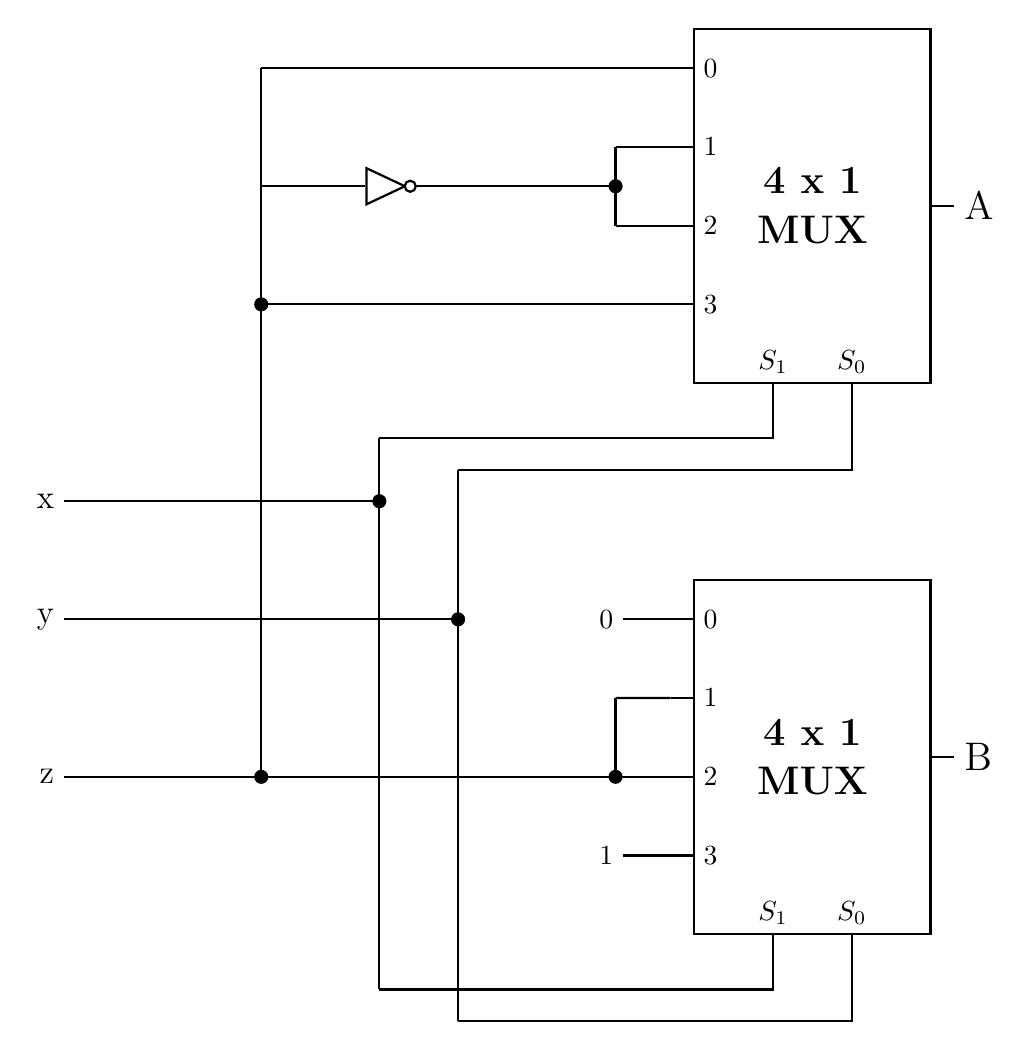
\begin{tikzpicture}[
    >=stealth,
    thick,
    dot/.style={circle, fill=black, inner sep=1.8pt, outer sep=0pt},
    every not gate US/.style={scale=1.3} % NOT gate-এর আকার ঠিক করার জন্য
]

% ==========================================
% 1. Custom 4x1 MUX Block Definition
% ==========================================
\tikzset{
    mux/.pic={
        % Main Box
        \draw (0,0) rectangle (3, 4.5);
        \node[align=center, font=\Large\bfseries] at (1.5, 2.25) {4 x 1 \\ MUX};
        
        % Data Input Pins (0, 1, 2, 3)
        \foreach \i/\y in {0/4, 1/3, 2/2, 3/1} {
            \node[anchor=west, font=\normalsize, inner sep=3pt] at (0, \y) {\i};
            \draw (0, \y) -- (-0.3, \y); % short pin line
            \coordinate (-in\i) at (-0.3, \y);
        }
        
        % Select Input Pins (S1, S0)
        \node[anchor=south, font=\normalsize, inner sep=3pt] at (1, 0) {$S_1$}; 
        \draw (1, 0) -- (1, -0.3);
        \coordinate (-s1) at (1, -0.3);
        
        \node[anchor=south, font=\normalsize, inner sep=3pt] at (2, 0) {$S_0$}; 
        \draw (2, 0) -- (2, -0.3);
        \coordinate (-s0) at (2, -0.3);
        
        % Output Pin
        \draw (3, 2.25) -- (3.3, 2.25);
        \coordinate (-out) at (3.3, 2.25);
    }
}

% ==========================================
% 2. Place MUX Components
% ==========================================
\pic (MuxA) at (8, 4.5) {mux};  % Top MUX
\pic (MuxB) at (8, -2.5) {mux}; % Bottom MUX

% Output Labels A and B
\node[right, font=\Large] at (MuxA-out) {A};
\node[right, font=\Large] at (MuxB-out) {B};

% ==========================================
% 3. Global Inputs (x, y, z)
% ==========================================
\node[left, font=\large] (varX) at (0, 3) {x};
\node[left, font=\large] (varY) at (0, 1.5) {y};
\node[left, font=\large] (varZ) at (0, -.5) {z};

% ==========================================
% 4. Routing Data Lines (Vertical Bus for x)
% ==========================================
\coordinate (Vx_bus) at (2.5, 0); % x-coordinate for the vertical x-bus

% Draw x line to the bus
\draw (varX.east) -- (4, 3) node[dot]{};

% Main vertical Vx bus line
\draw (2.5, 3) -- (2.5, 8.5); % Goes UP to Mux A
\draw (2.5, 3) -- (2.5, -0.5); % Goes DOWN to Mux B

% Connect MUX A Data Inputs to Vx bus
\draw (2.5, 8.5) -- (MuxA-in0); % Pin 0 (top bend, no dot)

\node[not gate US, draw] (not1) at (4, 7) {}; % Place NOT gate
\draw (2.5, 7)  -- (not1.input);   % Vx to NOT gate
\draw (not1.output)  -- (7,7)node[dot]{};              % NOT gate to Pin 1
\draw (7, 7.5)  -- (MuxA-in1);     % Pin 2
\draw (7,7.5) -- (7,6.5); 

\draw (7, 6.5)  -- (MuxA-in2);     % Pin 2
\draw (2.5, 5.5) node[dot]{} -- (MuxA-in3);     % Pin 3

% Connect MUX B Data Inputs
\draw (MuxA-in0 |- MuxB-in0) -- ++(-0.6, 0) node[left] {0}; % Pin 0 connected to 0
\draw (7, 0.5)  -- (MuxB-in1); 
\draw (7,0.5) -- (7,-0.5);                % Pin 1 to Vx
\draw (2.5, -0.5) node[dot]{} -- (MuxB-in2);                % Pin 2 to Vx
\draw (MuxA-in3 |- MuxB-in3) -- ++(-0.6, 0) node[left] {1}; % Pin 3 connected to 1

% ==========================================
% 5. Routing Select Lines (y, z)
% ==========================================
% Draw y and z horizontal lines to their respective vertical buses
\draw (varY.east) -- (5, 1.5) node[dot]{};
\draw (varZ.east) -- (7, -.5) node[dot]{};

% S1 Routing (connects to y)
\draw (MuxA-s1) |- (4, 3.8);   % Mux A S1 goes down and left
\draw (MuxB-s1) |- (4, -3.2);  % Mux B S1 goes down and left
\draw (4, 3.8) -- (4, -3.2);   % Vertical line combining them

% S0 Routing (connects to z)
\draw (MuxA-s0) |- (5, 3.4);   % Mux A S0 goes down and left
\draw (MuxB-s0) |- (5, -3.6);  % Mux B S0 goes down and left
\draw (5, 3.4) -- (5, -3.6);   % Vertical line combining them

\end{tikzpicture}
\end{center}

\mk{16} \yr{CSE 205 | L-2/T-1 | 2014--15}

\end{enumerate}


%% ══════════════════════════════════════════════════════════════════════
%%  SECTION 3: MINIMIZATION TECHNIQUES
%% ══════════════════════════════════════════════════════════════════════
\secdivider{Minimization Techniques}{K-Maps (2/3/4/5-variable), Quine-McCluskey, Don't-Care Conditions}{cC}{green}

\markboth{S3: Minimization Techniques}{S3: Minimization Techniques}
\label{sec:S3}
\titleformat{\section}{\large\bfseries\color{cC}}{}{0em}{}[\titlerule]
\section*{S3 \quad Minimization Techniques}
\addcontentsline{toc}{section}{S3: Minimization Techniques}

%%──────────────────────────────────────────────────────────────────────
\subtopic{cC}{Prime Implicants}
\label{sub:s3-prime-implicants}

\begin{enumerate}

%% -- Q1: Define prime implicants --
\item Define prime implicants.
\mk{3} \yr{CSE 205 | L-2/T-1 | 2011--12}


%% -- Q2: Prime implicants essential for 11-minterm function --
\item Find all the prime implicants for the following Boolean function and determine which are essential:
\[ F(A, B, C, D) = \Sigma\,(0, 2, 3, 5, 7, 8, 9, 10, 11, 13, 15) \]
\mk{11} \yr{CSE 205 | L-2/T-1 | 2014--15}

%% -- Q3: Differentiate prime implicant and essential prime implicant (2023-24) --
\item Differentiate between prime implicant and essential prime implicant of a K-Map.
\mk{7} \yr{CSE 205 | L-2/T-1 | 2023--24}

\end{enumerate}

%%──────────────────────────────────────────────────────────────────────
\subtopic{cC}{Karnaugh Map}
\label{sub:s3-kmap}

\begin{enumerate}

%% -- Q1: K-Map SOP and POS with don't cares --
\item Minimize the following function in both SOP and POS forms using Karnaugh map:
\[ f(A,B,C,D) = \Sigma\,m(0,4,7,9,13) + d(5,8,15) \]
\mk{12} \yr{CSE 205 | L-2/T-1 | 2012--13}

%% -- Q2: K-Map two functions --
\item Simplify the following Boolean functions using K-map:
\begin{enumerate}
  \item $F(A,B,C,D) = AB'C + A'B'D' + ABD + ACD' + AB'C' + A'BC'D$
  \item $F(A,B,C,D) = \Sigma\,(0,2,5,7,8,15)$ with don't-care conditions $d(A,B,C,D) = \Sigma\,(10,14)$

  \end{enumerate}
\mk{15} \yr{CSE 205 | L-2/T-1 | 2013--14}
%% -- Q3: K-map POS simplification with don't cares --
\item Using K-maps, find the simplified product of sums form of the following Boolean function:
\[ f(w, x, y, z) = \Sigma\,(1, 5, 8, 12, 14, 15), \quad \text{don't-care minterms: } d = \Sigma\,(3, 11) \]
\mk{10} \yr{CSE 205 | L-2/T-1 | 2015--16}


%% -- Q4: K-map SOP 6-variable with don't cares --
\item Using K-maps, find the simplified sum of products form of the following Boolean function:
\[ f(a,b,c,d,e,f) = \Sigma\,(1,2,3,5,7,11,13,17,19,23,29,31) \]
Don't-care minterms: $d = \Sigma\,(6,20,24,25,26,27)$.
\mk{12} \yr{CSE 205 | L-2/T-1 | 2015--16}


%% -- Q5: 5-variable K-map with don't cares; essential PIs (2016-17) --
\item Using K-map, solve $f(x_1,x_2,x_3,x_4,x_5) = \Sigma\,(0,2,4,5,6,7,8,10,14,17,18,21,29,31) + d\Sigma\,(11,20,22)$. Find the essential prime implicants. (Show the reduction steps.)
\mk{15} \yr{CSE 205 | L-2/T-1 | 2016--17}

%% -- Q6: 5-variable K-map (2020-21) --
\item Using K-Map, minimize $f(v,w,x,y,z) = \Sigma\,(2,7,8,15,22,23,25,29) + d(6,9,13,18,24,31)$. Find the Prime Implicants and Essential Prime Implicants, and the Minimal Sums. Write down the responsible minterm for each Essential Prime Implicant.
\mk{15} \yr{CSE 205 | L-2/T-1 | 2020--21}


%% -- Q7: K-Map minimize with don't cares; PIs, EPIs, responsible minterms (2017-18) --
\item Using K-Map, minimize $f(w,x,y,z) = \mathrm{SOP}(1,2,4,7,9,10,12,14) + d(0,6,8,13)$. Find the Prime Implicants and Essential Prime Implicants. Write down the responsible minterm for each Essential Prime Implicant.
\mk{12} \yr{CSE 205 | L-2/T-1 | 2017--18}

%% -- Q8: K-Map minimize with don't cares; PIs, EPIs (2018-19) --
\item Using K-Map, minimize $f(w,x,y,z) = \Sigma\,(1,2,3,7,10,12,14) + d(0,6,8,13)$. Find the Prime Implicants and Essential Prime Implicants. Write down the responsible minterm for each Essential Prime Implicant.
\mk{12} \yr{CSE 205 | L-2/T-1 | 2018--19}


%% -- Q9: SOP to simplified POS; draw logic circuit (2019-20) --
\item Convert the following Boolean function from sum-of-products form to a simplified product-of-sums form, then draw a logic circuit for the POS form:
\[ F(w,x,y,z) = \Sigma\,(0,1,2,5,7,11,13) \]
\mk{20} \yr{CSE 205 | L-2/T-1 | 2019--20}



\end{enumerate}

%%──────────────────────────────────────────────────────────────────────
\subtopic{cC}{Tabulation Method (Quine-McCluskey)}
\label{sub:s3-tabulation}

\begin{enumerate}

%% -- Q1: Tabulation method --
\item Simplify the following Boolean function by using the tabulation method:
\[ F(A,B,C,D) = \Sigma\,(0,1,2,8,10,11,14,15) \]
\mk{15} \yr{CSE 205 | L-2/T-1 | 2011--12}


%% -- Q2: When to prefer tabulation over K-map --
\item When is the tabulation method more preferable than the K-Map method for simplifying a Boolean function?
\mk{5} \yr{CSE 205 | L-2/T-1 | 2014--15}


%% -- Q3: Q-M method 5-variable, essential PIs --
\item Minimize the following function using the Quine-McCluskey (Q-M) method. Find essential prime implicants and all prime implicants:
\[ f(A,B,C,D,E) = \Sigma\,(0,1,2,8,9,15,17,21,24,25,27,31) \]
\mk{20} \yr{CSE 205 | L-2/T-1 | 2016--17}


%% -- Q4: Compare tabulation and K-map methods: merits and demerits (2019-20) --
\item Compare the Tabulation method and the Karnaugh map for minimizing Boolean functions based on their merits and demerits.
\mk{15} \yr{CSE 205 | L-2/T-1 | 2019--20}


%% -- Q5: Tabulation method; find essential PIs (2019-20) --
\item Using the Tabulation method, simplify the following Boolean function by first finding the essential prime implicants:
\[ F(A,B,C,D) = \Sigma\,(1,3,4,5,10,11,12,13,14) \]
\mk{28} \yr{CSE 205 | L-2/T-1 | 2019--20}

%% -- Q6: Find prime implicants using tabulation method F(w,x,y,z)=Σ(0,1,2,8,10,11,14,15) (2021-22) --
\item Determine the prime implicants of the following function using the tabulation (tabular) method:
\[ F(w, x, y, z) = \Sigma\,(0, 1, 2, 8, 10, 11, 14, 15) \]
\mk{15} \yr{CSE 205 | L-2/T-1 | 2021--22}

%% -- Q7: Tabular method; prime and essential prime implicants (2022-23) --
\item Using tabular method, find the prime implicants and essential prime implicants of the following Boolean function:
\[ F(A, B, C, D) = \Sigma\,(0, 2, 3, 5, 7, 8, 9, 10, 11, 13, 15) \]
\mk{15} \yr{CSE 205 | L-2/T-1 | 2022--23}

%% -- Q8: Simplify to SOP and POS form (2022-23) --
\item Simplify the following Boolean function into (a) sum-of-products form and (b) product-of-sums form:
\[ F(A, B, C, D) = \Sigma\,(0, 1, 2, 5, 8, 9, 10) \]
\mk{14} \yr{CSE 205 | L-2/T-1 | 2022--23}

%% -- Q9: Simplify to POS form; purpose of Q-M method (2024-25) --
\item Simplify the following Boolean function to product-of-sums form:
\[ F = \Sigma\,(3,4,6,7,9,11,12,14,15) \]
What is the main purpose of the tabulation method (Quine-McCluskey method) in digital logic design, and how does it systematically help in minimizing Boolean expressions compared to the Karnaugh map method?
\mk{15} \yr{CSE 205 | L-2/T-1 | 2024--25}

\end{enumerate}

%%──────────────────────────────────────────────────────────────────────
\subtopic{cC}{NAND-Only \& NOR-Only Implementation (Minimization Context)}
\label{sub:s3-nand-impl}

\begin{enumerate}

%% -- Q1: Simplify F(w,x,y,z) and draw using only NAND gates (2023-24) --
\item Simplify the following function and draw the circuit using only NAND gates:
\[ F(w,x,y,z) = \Sigma\,(0,1,2,4,5,6,8,9,12,13,14) \]
\mk{16} \yr{CSE 205 | L-2/T-1 | 2023--24}

%% -- Q2: Implement using NAND-AND gates (2023-24) --
\item Implement $F(x,y,z) = x'y'z' + xyz'$ using two-level forms of logic by using NAND-AND gates. Assume that the complement of $x$, $y$ and $z$ are readily available.
\mk{14} \yr{CSE 205 | L-2/T-1 | 2023--24}

\end{enumerate}


%% ══════════════════════════════════════════════════════════════════════
%%  SECTION 4: COMBINATIONAL LOGIC
%% ══════════════════════════════════════════════════════════════════════
\secdivider{Combinational Logic}{Adders, Subtractors, Comparators, Decoders, Encoders, MUX, DEMUX}{cD}{violet}

\markboth{S4: Combinational Logic}{S4: Combinational Logic}
\label{sec:S4}
\titleformat{\section}{\large\bfseries\color{cD}}{}{0em}{}[\titlerule]
\section*{S4 \quad Combinational Logic}
\addcontentsline{toc}{section}{S4: Combinational Logic}

%%──────────────────────────────────────────────────────────────────────
\subtopic{cD}{Code Converter}
\label{sub:s4-code-converter}

\begin{enumerate}

%% -- Q1: Random Code to BCD using K-Map (2021-22) --
\item Design a combinational circuit that converts a decimal digit represented with ``Random Code'' to ``BCD Code'' (see Table~1). Use the K-Map method for logic simplification and show the circuit diagram.

\begin{center}
  \begin{tabular}{|c|c|c|}
\hline
Decimal Digit & \begin{tabular}{@{}c@{}}Random Code \\ ABCD\end{tabular} & \begin{tabular}{@{}c@{}}BCD Code \\ wxyz\end{tabular} \\
\hline
0 & 0000 & 0000 \\ \hline
1 & 0011 & 0001 \\ \hline
2 & 0101 & 0010 \\ \hline
3 & 0110 & 0011 \\ \hline
4 & 1010 & 0100 \\ \hline
5 & 1011 & 0101 \\ \hline
6 & 1100 & 0110 \\ \hline
7 & 1101 & 0111 \\ \hline
8 & 1110 & 1000 \\ \hline
9 & 1111 & 1001 \\ \hline
\end{tabular}
\end{center}

\mk{20} \yr{CSE 205 | L-2/T-1 | 2021--22}

%% -- Q2: Gray to Binary Code Converter using minimum gates (2022-23) --
\item Design a combinational circuit that converts a three-bit gray code to a three-bit binary number. Use only a minimum number of gates in your design.
\mk{20} \yr{CSE 205 | L-2/T-1 | 2022--23}

%% -- Q3: Consensus circuit: output=1 if exactly two inputs are 1 (2023-24) --
\item A consensus circuit is a combinational circuit whose output is equal to 1 if exactly two inputs are 1, and 0 otherwise. Design a 3-input consensus circuit by finding the circuit's truth table, simplified Boolean equation and a circuit diagram.
\mk{12} \yr{CSE 205 | L-2/T-1 | 2023--24}

%% -- Q4: Magnitude comparator for two 3-bit numbers (2024-25) --
\item Design a magnitude comparator for comparing two 3-bit binary numbers $X$ and $Y$.
\mk{14} \yr{CSE 205 | L-2/T-1 | 2024--25}

\end{enumerate}

%%──────────────────────────────────────────────────────────────────────
\subtopic{cD}{Number System \& Arithmetic Operations}
\label{sub:s4-number-sys}

\begin{enumerate}

%% -- Q1: Decimal to binary conversion --
\item Convert $(41.6875)_{10}$ to binary.
\mk{5} \yr{CSE 205 | L-2/T-1 | 2011--12}

%% -- Q2: Binary subtraction using 1s and 2s complement --
\item Perform the subtraction with the following binary unsigned numbers using (i) 2's complement, (ii) 1's complement: $11010 - 1101$.
\mk{10} \yr{CSE 205 | L-2/T-1 | 2011--12}

%% -- Q3: Direct binary subtraction --
\item Perform the following binary subtraction: $11000011 - 10101010$.
\mk{6} \yr{CSE 205 | L-2/T-1 | 2012--13}

%% -- Q4: 2s complement subtract decimals --
\item Using 2's complement, subtract decimal $-70$ from decimal $-50$.
\mk{9} \yr{CSE 205 | L-2/T-1 | 2012--13}

\end{enumerate}

%%──────────────────────────────────────────────────────────────────────
\subtopic{cD}{Binary Adder \& Subtractor}
\label{sub:s4-adder-sub}

\begin{enumerate}

%% -- Q1: Full subtractor from truth table --
\item Starting with a truth table, design a full subtractor.
\mk{20} \yr{CSE 205 | L-2/T-1 | 2012--13}

%% -- Q2: 4-bit adder and subtractor --
\item Design a four-bit binary adder using a 1-bit full-adder circuit. How can it be modified to use as a four-bit subtractor?
\mk{15} \yr{CSE 205 | L-2/T-1 | 2013--14}


%% -- Q3: 4-bit BCD adder design --
\item Design a 4-bit BCD adder using 4-bit binary adders and basic logic gates. Use a block diagram to draw a binary adder.
\mk{15} \yr{CSE 205 | L-2/T-1 | 2014--15}


%% -- Q4: Advantages and disadvantages of serial and parallel adders --
\item Write the advantages and disadvantages of serial and parallel adders.
\mk{4} \yr{CSE 205 | L-2/T-1 | 2015--16}


%% -- Q5: Full subtractor circuit: x - y - Bin; outputs Diff and Bout (2019-20) --
\item Design a full subtractor circuit with three inputs $x$, $y$, $B_{in}$ and two outputs $\mathrm{Diff}$ and $B_{out}$. The circuit subtracts $x - y - B_{in}$, where $B_{in}$ is the input borrow and $B_{out}$ is the output borrow.
\mk{18} \yr{CSE 205 | L-2/T-1 | 2019--20}

%% -- Q6: 4-bit binary subtractor using full adders; 2's complement explanation (2024-25) --
\item Design a 4-bit binary subtractor circuit using full adders.
\begin{enumerate}
  \item Construct and draw the logic diagram of the subtractor circuit.
  \item Explain how subtraction is performed using 2's complement representation.(Understand level)
\end{enumerate}
\mk{15} \yr{CSE 205 | L-2/T-1 | 2024--25}

\end{enumerate}

%%──────────────────────────────────────────────────────────────────────
\subtopic{cD}{BCD Adder-Subtractor}
\label{sub:s4-bcd-addsub}

\begin{enumerate}

%% -- Q1: Combined BCD A+B and A-B circuit (2016-17) --
\item Design a circuit which computes $A - B$ and $A + B$ where $A$ and $B$ are 4-bit BCD values. Explain the design.
\mk{15} \yr{CSE 205 | L-2/T-1 | 2016--17}

%% -- Q2: BCD adder-subtractor with selector bit (2017-18) --
\item Design a BCD adder-subtractor for two BCD inputs $A$ and $B$. Addition and subtraction is selected by a selector bit $x$: when $x=0$ the circuit computes $A+B$; when $x=1$ it computes $A-B$. Explain the operations $9+7$ and $9-7$ with your designed circuit.
\mk{9+4} \yr{CSE 205 | L-2/T-1 | 2017--18}

%% -- Q3: BCD adder-subtractor with selector bit S (2020-21) --
\item Design a BCD adder-subtractor which takes two 4-bit BCD numbers $A$ and $B$. Addition and subtraction is selected by a selector bit $S$: when $S=0$ the circuit produces $A+B$; when $S=1$ it produces $A-B$.
\mk{12} \yr{CSE 205 | L-2/T-1 | 2020--21}

\end{enumerate}

%%──────────────────────────────────────────────────────────────────────
\subtopic{cD}{Carry Look-Ahead Adder (CLA)}
\label{sub:s4-cla}

\begin{enumerate}

%% -- Q1: CLA advantages and propagation delay --
\item What are the advantages of a CLA over a normal binary four-bit adder? Assume that the exclusive-OR gate has a propagation delay of 10\,ns and that the AND or OR gates have a propagation delay of 5\,ns. What is the total propagation delay time in the four-bit CLA adder?
\mk{10} \yr{CSE 205 | L-2/T-1 | 2013--14}


%% -- Q2: CLA problem with parallel adder; design 4-bit CLA; delay (1ns NOT, 2ns others) --
\item What is the problem with the binary parallel adder circuit? Design and implement a 4-bit carry look-ahead adder circuit. If the propagation delay is 1\,ns for a NOT gate and 2\,ns for other basic gates, what is the propagation delay of the CLA adder to produce its final output?
\mk{18} \yr{CSE 205 | L-2/T-1 | 2015--16}


%% -- Q3: CLA advantage + propagation delay (NOT=2ns, others=4ns) --
\item For a carry look-ahead adder circuit, what advantage do we get if we use it instead of a 4-bit simple full adder? For a NOT gate with 2\,ns propagation delay and other basic gates with 4\,ns propagation delay, what will be the total propagation delay?
\mk{5} \yr{CSE 205 | L-2/T-1 | 2016--17}

%% -- Q4: 3-bit CLA; show all types of carry for 3+4 --
\item Design a 3-bit CLA circuit and show all types of ``carry'' for the addition $3+4$ with your designed CLA.
\mk{8+4} \yr{CSE 205 | L-2/T-1 | 2017--18}

\item Design a 4 bit Carry Look Ahead (CLA) adder which will take $X_3X_2X_1X_0$ and $Y_3Y_2Y_1Y_0$ as input, and produce their sum. Show the steps and the role of different \textit{carries} of this CLA.
\mk{13} \yr{CSE 205 | L-2/T-1 | 2020--21}

%% -- Q6: Benefits of CLA; derive carry expressions (2023-24) --
\item What is the benefit of using an adder with carry lookahead logic? Derive expressions of different carry of a 4-bit adder with carry lookahead logic.
\mk{15} \yr{CSE 205 | L-2/T-1 | 2023--24}

%% -- Q7: CLA working principle; derive C1,C2,C3,C4 (2024-25) --
\item Explain the working principle of a Carry Look-Ahead (CLA) adder. Derive the expressions for carry generation ($C_1, C_2, C_3, C_4$) using generate and propagate functions.
\mk{12} \yr{CSE 205 | L-2/T-1 | 2024--25}

\end{enumerate}

%%──────────────────────────────────────────────────────────────────────
\subtopic{cD}{2's Complement Circuit}
\label{sub:s4-2scomp}

\begin{enumerate}

%% -- Q1: 4-bit 2s complement circuit --
\item Design a circuit that takes a 4-bit number as input and produces the 2's complement of the given number.
\mk{20} \yr{CSE 205 | L-2/T-1 | 2011--12}

%% -- Q2: 1's complementer using only half adders; C=1 complement, C=0 pass (2023-24) --
\item Using only half adders, design a circuit that outputs the 1's complement of a 4-bit input when the control input $C$ is 1, and passes the input unchanged when $C$ is 0.
\mk{6} \yr{CSE 205 | L-2/T-1 | 2023--24}

\end{enumerate}

%%──────────────────────────────────────────────────────────────────────
\subtopic{cD}{Overflow Detection}
\label{sub:s4-overflow}

\begin{enumerate}

%% -- Q1: Overflow in signed and unsigned --
\item How do you check for overflow in the case of addition of two binary numbers in both signed and unsigned representations?
\mk{5} \yr{CSE 205 | L-2/T-1 | 2013--14}

%% -- Q2: Overflow in signed addition and subtraction; examples (2024-25) --
\item What is overflow in binary arithmetic? Explain how overflow is detected in signed addition and signed subtraction. Provide suitable examples.
\mk{11} \yr{CSE 205 | L-2/T-1 | 2024--25}

\end{enumerate}

%%──────────────────────────────────────────────────────────────────────
\subtopic{cD}{Binary Multiplier}
\label{sub:s4-multiplier}

\begin{enumerate}

%% -- Q1: 2x2 binary multiplier circuit --
\item The figure below represents a multiplier that takes two 2-bit binary numbers $x_1x_0$ and $y_1y_0$ as inputs, and produces an output binary number $p_3p_2p_1p_0$ equal to the arithmetic product of the two input numbers. Design the logic circuit for the multiplier.
\mk{20} \yr{CSE 205 | L-2/T-1 | 2012--13}

\begin{center}
  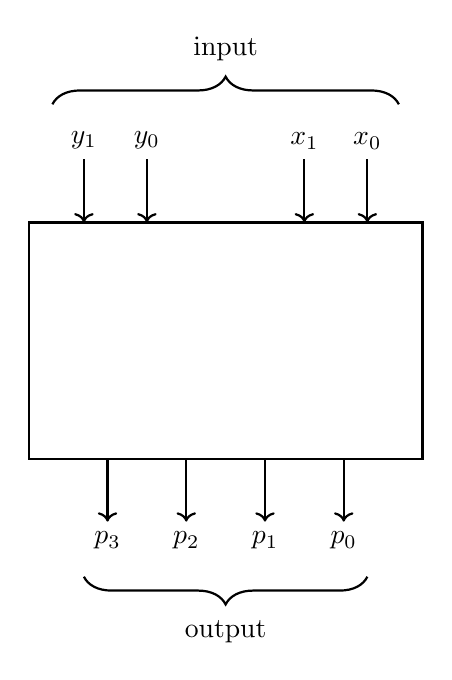
\begin{tikzpicture}
        
        % Main Box
        \draw[thick] (-2.5, -1.5) rectangle (2.5, 1.5);
        
        % Input Arrows and Labels
        \draw[->, thick] (-1.8, 2.3) node[above] {$y_1$} -- (-1.8, 1.5);
        \draw[->, thick] (-1.0, 2.3) node[above] {$y_0$} -- (-1.0, 1.5);
        \draw[->, thick] (1.0, 2.3) node[above] {$x_1$} -- (1.0, 1.5);
        \draw[->, thick] (1.8, 2.3) node[above] {$x_0$} -- (1.8, 1.5);
        
        % Top Curly Brace for "input"
        \draw[decorate, decoration={brace, amplitude=10pt}, thick] 
            (-2.2, 3) -- (2.2, 3) node[midway, above=12pt] {input};

        % Output Arrows and Labels
        \draw[->, thick] (-1.5, -1.5) -- (-1.5, -2.3) node[below] {$p_3$};
        \draw[->, thick] (-0.5, -1.5) -- (-0.5, -2.3) node[below] {$p_2$};
        \draw[->, thick] (0.5, -1.5) -- (0.5, -2.3) node[below] {$p_1$};
        \draw[->, thick] (1.5, -1.5) -- (1.5, -2.3) node[below] {$p_0$};
        
        % Bottom Curly Brace for "output"
        \draw[decorate, decoration={brace, amplitude=10pt, mirror}, thick] 
            (-1.8, -3) -- (1.8, -3) node[midway, below=12pt] {output};
            
    \end{tikzpicture}
\end{center}

%% -- Q2: 1-bit by 1-bit multiplier --
\item How would you implement a one-bit by one-bit binary multiplier using basic gates?
\mk{5} \yr{CSE 205 | L-2/T-1 | 2013--14}


%% -- Q3: 3-bit multiplier using 4-bit adders --
\item Using 4-bit adders, design a 3-bit multiplier for 3-bit variables $X(X_1,X_2,X_3)$ and $Y(Y_1,Y_2,Y_3)$. Explain the design.
\mk{15} \yr{CSE 205 | L-2/T-1 | 2016--17}

%% -- Q4: 3-bit multiplier using 4-bit adder (circuit) --
\item Design a circuit with a 4-bit binary adder which returns $A \times B$ where $A$ and $B$ are 3-bit binary numbers.
\mk{10} \yr{CSE 205 | L-2/T-1 | 2018--19}

%% -- Q5: 2-bit by 2-bit binary multiplier design (2021-22) --
\item Discuss and design a 2-bit by 2-bit binary multiplier.
\mk{15} \yr{CSE 205 | L-2/T-1 | 2021--22}

\end{enumerate}

%%──────────────────────────────────────────────────────────────────────
\subtopic{cD}{Incrementer}
\label{sub:s4-incrementer}

\begin{enumerate}

%% -- Q1: 4-bit incrementer using half-adders --
\item Design a 4-bit incrementer circuit using 4 half-adders. Note that the incrementer circuit adds 1 to a binary number.
\mk{10} \yr{CSE 205 | L-2/T-1 | 2011--12}

%% -- Q2: 4-bit combinational incrementer using only half adders (2021-22) --
\item Design a 4-bit combinational circuit incrementer (a circuit that adds 1 to a 4-bit binary number) using only half adders.
\mk{10} \yr{CSE 205 | L-2/T-1 | 2021--22}

\end{enumerate}

%%──────────────────────────────────────────────────────────────────────
\subtopic{cD}{Encoders \& Decoders}
\label{sub:s4-encoders}

\begin{enumerate}

%% -- Q1: 4-input priority encoder (default priority) --
\item Design a 4-input priority encoder and show the gate-level circuit diagram.
\mk{12} \yr{CSE 205 | L-2/T-1 | 2011--12, 2013--14}

%% -- Q2: Priority encoder with custom priority order --
\item What is a priority encoder? Design a four-input priority encoder with inputs $I_0, I_1, I_2, I_3$, where the priority order is $I_2 > I_3 > I_1 > I_0$.
\mk{10} \yr{CSE 205 | L-2/T-1 | 2013--14}

%% -- Q3: 3x8 decoder from two 2x4 decoders --
\item Design a $3 \times 8$ decoder using two $2 \times 4$ decoder circuits.
\mk{8} \yr{CSE 205 | L-2/T-1 | 2011--12}

%% -- Q4: Decoder as full adder --
\item You need a full adder for an experiment but in the lab you could only find plenty of $3 \times 8$ decoders. Can any such decoder be used as a full adder? Explain your answer with a truth table.
\mk{15} \yr{CSE 205 | L-2/T-1 | 2012--13}


%% -- Q3: Full adder with decoder --
\item Design a full adder with a decoder and basic logic gates.
\mk{12} \yr{CSE 205 | L-2/T-1 | 2014--15}

%% -- Q4: Octal-to-binary encoder ambiguity --
\item An Octal-to-Binary Encoder may cause ambiguities if more than one input is simultaneously set to~1. How can this ambiguity be resolved?
\mk{4} \yr{CSE 205 | L-2/T-1 | 2014--15}


%% -- Q5: Priority encoder 9-bit, negative enable, lower order gets priority --
\item ``A lower-order code will get priority'' --- Design and explain a priority encoder with negative enable for 9 bits.
\mk{10} \yr{CSE 205 | L-2/T-1 | 2016--17}

%% -- Q6: 8-to-3 priority encoder, custom priority order (2017-18) --
\item Design an 8-to-3 priority encoder with the priority order: 6, 0, 7, 4, 5, 3, 1, 2 (6 has highest priority, 2 has lowest priority).
\mk{13} \yr{CSE 205 | L-2/T-1 | 2017--18}

%% -- Q7: 8-to-3 priority encoder, custom priority order (2018-19) --
\item Design an 8-to-3 priority encoder with the priority order: 5, 0, 7, 4, 6, 3, 2, 1 (5 has highest priority, 1 has lowest priority).
\mk{13} \yr{CSE 205 | L-2/T-1 | 2018--19}

%% -- Q8: Priority encoder for 8 colleges (2020-21) --
\item After a school final result, Ishrat applied for college admission and gave her choices from eight colleges indexed A to H, following the priority order B, A, D, E, F, H, G, C (B has the highest priority, C has the lowest priority). Find the Boolean function of her choices and show the design steps.
\mk{15} \yr{CSE 205 | L-2/T-1 | 2020--21}

%% -- Q9: 8-to-3 priority encoder lower priority given to lower input (2023-24) --
\item Show the truth table of an 8-to-3 line priority encoder, where higher priority is given to lower numbered input.
\mk{9} \yr{CSE 205 | L-2/T-1 | 2023--24}

%% -- Q10: Light sensor controller for 8 servers with priority (2024-25) --
\item Design a light sensor based controller circuit for accessing eight servers A, B, C, D, E, F, G, H. The light sensors are numbered as $S_1, S_2, \ldots$ and so on. The sensors of the controller will be ON to show which server is active. The servers have some priority order: C, A, E, H, D, G, F, B (C has the highest priority and B has the lowest priority).
\mk{15} \yr{CSE 205 | L-2/T-1 | 2024--25}

\end{enumerate}

%%──────────────────────────────────────────────────────────────────────
\subtopic{cD}{Function Implementation using Decoder}
\label{sub:s4-decoder-func}

\begin{enumerate}

%% -- Q1: 3x8 active-low decoder for two 4-var functions --
\item Consider a $3 \times 8$ decoder whose outputs are active low and which has one active high enable signal. Implement the following functions using the above-mentioned decoder:
\begin{enumerate}
  \item $f(a,b,c,d) = \Pi\,(3,5,14)$
  \item $f(a,b,c,d) = \Sigma\,(1,6,8,13)$
  
  \end{enumerate}
Note that you will need to implement both functions in a single circuit. You may use as many decoders as required, keeping the implementation as efficient as possible. Basic gates are also allowed.
\mk{13} \yr{CSE 205 | L-2/T-1 | 2015--16}


%% -- Q2: f=π(3,5,9,15,12,4,1) with active-low 2x4 decoder --
\item Using only a $2 \times 4$ line decoder, solve the function $f(A,B,C,D) = \pi\,(3,5,9,15,12,4,1)$. The $2\times4$ line decoder has an active-low enable and active-low outputs. (Use the minimum number of gates if required.)
\mk{10} \yr{CSE 205 | L-2/T-1 | 2016--17}

%% -- Q3: f(w,x,y,z) with 2x4 decoder A,B input, active-low EN, active-low outputs --
\item Design a logic circuit for $f(w, x, y, z) = \mathrm{SOP}(0, 2, 6, 7, 8, 10, 11, 13, 14)$ with a $2\times4$ line decoder that has inputs $A$, $B$, active-low enable $\overline{EN}$ and active-low outputs $D_0', D_1', D_2', D_3'$. (Use the minimum number of extra logic gates.)
\mk{12} \yr{CSE 205 | L-2/T-1 | 2017--18}

%% -- Q4: f(w,x,y,z) with 2x4 decoder, two active-low enables (2018-19) --
\item Design a logic circuit for $f(w, x, y, z) = \Sigma\,(0, 2, 6, 7, 10, 11, 12, 14)$ with a $2\times4$ line decoder that has inputs $A$, $B$, active-low enables $\overline{EN_1}$ and $\overline{EN_2}$. (Use the minimum number of extra logic gates.)
\mk{14} \yr{CSE 205 | L-2/T-1 | 2018--19}

%% -- Q5: Full adder with 2x4 decoder (half subtractor) --
\item Using a $2 \times 4$ line decoder, design a half subtractor. (Decoder outputs $D_0, D_1, D_2, D_3$ are active high; enable $\overline{EN}$ is active low.)
\mk{10} \yr{CSE 205 | L-2/T-1 | 2017--18}

%% -- Q6: Two 2-bit numbers sum with 2x4 decoder (2020-21) --
\item Design a logic circuit which takes two 2-bit numbers $X_1X_0$ and $Y_1Y_0$ and finds their sum using a $2\times4$ line decoder with inputs $I_0, I_1$, active-low outputs $O_3, O_2, O_1, O_0$, and active-low enables $\overline{EN_1}$ and $\overline{EN_2}$. (Use the minimum number of extra logic gates.)
\mk{15} \yr{CSE 205 | L-2/T-1 | 2020--21}

%% -- Q7: F(x,y,z)=Σ(3,5,6,7) with active-low 3x8 decoder and AND gates (2021-22) --
\item Implement $F(x, y, z) = \Sigma\,(3, 5, 6, 7)$ using an active low $3 \times 8$ decoder and AND gates.
\mk{10} \yr{CSE 205 | L-2/T-1 | 2021--22}

%% -- Q8: Full adder with 3x8 decoder and two OR gates (2022-23) --
\item Design a full adder circuit using a $3 \times 8$ decoder and two OR gates.
\mk{10} \yr{CSE 205 | L-2/T-1 | 2022--23}

%% -- Q9: 4-to-16 decoder from minimum number of 2-to-4 decoders (2023-24) --
\item Design a 4-to-16-line decoder by using only the minimum number of 2-to-4-line decoders. Assume that the 2-to-4-line decoders have an enable input (`1' = enabled) but the designed 4-to-16-line decoder does not have an enable input.
\mk{12} \yr{CSE 205 | L-2/T-1 | 2023--24}

%% -- Q10: 1-bit full subtractor using 4-to-16 decoder with active-low outputs (2024-25) --
\item Design a 1-bit full subtractor using a 4 to 16 line decoder that has active low outputs and two active low enables $\overline{EN_1}$ and $\overline{EN_2}$.
\mk{12} \yr{CSE 205 | L-2/T-1 | 2024--25}

\end{enumerate}

%%──────────────────────────────────────────────────────────────────────
\subtopic{cD}{Decoder as Demultiplexer}
\label{sub:s4-demux}

\begin{enumerate}
  

%% -- Q1: Decoder as demultiplexer explanation (2016-17) --
\item How can a decoder be used as a demultiplexer? Explain with an example.
\mk{5} \yr{CSE 205 | L-2/T-1 | 2016--17}

%% -- Q2: Show decoder acts as demultiplexer (2018-19) --
\item Show that a decoder can be used as a demultiplexer.
\mk{8} \yr{CSE 205 | L-2/T-1 | 2018--19}

%% -- Q3: Decoder as demultiplexer (2020-21) --
\item Can a decoder act like a demultiplexer? If yes, explain how.
\mk{5} \yr{CSE 205 | L-2/T-1 | 2020--21}

%% -- Q4: What is a demultiplexer; give an example (2021-22) --
\item What is a demultiplexer? Give an example.
\mk{8} \yr{CSE 205 | L-2/T-1 | 2021--22}


\end{enumerate}

%%──────────────────────────────────────────────────────────────────────
\subtopic{cD}{BCD to 7-Segment Decoder \& BCD Error Detector}
\label{sub:s4-bcd}

\begin{enumerate}

%% -- Q1: RBI and RBO connection for leading zeros --
\item Explain how the Ripple-blanking input (RBI) and Ripple-blanking output (RBO) pins of the BCD to 7-segment decoder (IC 7447) should be connected such that all but the LSB show blank for leading zeros.
\mk{6} \yr{CSE 205 | L-2/T-1 | 2012--13}

%% -- Q2: BCD error detector design --
\item You are receiving BCD codes sent by a remote transmitter. The bits are $A_3A_2A_1A_0$ ($A_0$ being the LSB). Design a BCD-error-detector (BED) for your receiver that will produce a HIGH for any received code that is not a valid BCD code. (For example, if you receive $1010$, the output of BED will be HIGH.)
\mk{15} \yr{CSE 205 | L-2/T-1 | 2012--13}

\end{enumerate}

%%──────────────────────────────────────────────────────────────────────
\subtopic{cD}{Multiplexers \& Demultiplexers}
\label{sub:s4-mux}

\begin{enumerate}

%% -- Q1: 4x1 MUX function implementation --
\item Implement the following function $F$ using one $4 \times 1$ multiplexer and basic gates:
\[ F(A,B,C,D) = \Sigma\,(1,3,4,11,12,13,14,15) \]
\mk{15} \yr{CSE 205 | L-2/T-1 | 2011--12}

%% -- Q2: 16-to-1 MUX implementation --
\item Implement $F = \Sigma\,(3,5,7,10,11,13,14,15)$ using a 16-to-1 MUX.
\mk{10} \yr{CSE 205 | L-2/T-1 | 2012--13}

%% -- Q3: 4-to-1 MUX feasibility --
\item Can the function $F = \Sigma\,(3,5,7,10,11,13,14,15)$ be implemented using only one $4 \times 1$ MUX? If yes, show how; if not, explain why.
\mk{10} \yr{CSE 205 | L-2/T-1 | 2012--13}

%% -- Q4: 8x1 MUX Boolean function determination --
\item An $8 \times 1$ multiplexer has inputs $A, B, C, D$ where inputs $A$, $B$, and $C$ are connected to selection inputs $S_2$, $S_1$, and $S_0$ respectively. The data inputs $I_0$ through $I_7$ are: $I_1 = I_2 = 0$; $I_3 = I_7 = 1$; $I_4 = I_5 = D$; $I_0 = I_6 = D'$. Determine the Boolean function that the multiplexer implements.
\mk{15} \yr{CSE 205 | L-2/T-1 | 2013--14}

%% -- Q5: 16x1 MUX from 8x1 and 2x1 --
\item Construct a $16 \times 1$ multiplexer with two $8 \times 1$ and one $2 \times 1$ multiplexers.
\mk{5} \yr{CSE 205 | L-2/T-1 | 2013--14}


%% -- Q5: Three-state buffer truth table and 2-to-1 MUX --
\item Show the truth table for a three-state buffer. Construct a 2-to-1 line MUX with three-state buffers.
\mk{3+5} \yr{CSE 205 | L-2/T-1 | 2014--15}


%% -- Q6: Full subtractor using 2x1 MUX only --
\item Design and implement the circuit diagram of a 1-bit full subtractor circuit using $2\times1$ MUXs only. You cannot use any other gates.
\mk{12} \yr{CSE 205 | L-2/T-1 | 2015--16}


%% -- Q7: 4x1 MUX for f(w,x,y,z)=Π(2,4,5,7,11,12,13) --
\item Consider the Boolean function $f(w, x, y, z) = \Pi\,(2,4,5,7,11,12,13)$. Implement the function using a $4 \times 1$ MUX and other basic gates if necessary.
\mk{10} \yr{CSE 205 | L-2/T-1 | 2015--16}


%% -- Q8: f(w,x,y,z)=π(2,4,5,7,11,12,13) with 4x1 MUX (2016-17) --
\item Using only $4\times1$ line, 2-bit multiplexers, design $f(w,x,y,z) = \pi\,(2,4,5,7,11,12,13)$. (Use minimum gates if required.)
\mk{12} \yr{CSE 205 | L-2/T-1 | 2016--17}

%% -- Q9: 8x1 MUX for POS function with active-low EN (2017-18) --
\item Using an $8\times1$ line MUX, design a logic circuit for $f(w,x,y,z) = \mathrm{POS}(0,2,5,6,7,8,9,10)$, where the MUX has selector bits $S_2S_1S_0$, input lines $I_0\ldots I_7$, and active-low enable $\overline{EN}$. (If $S_2S_1S_0 = 000$, $I_0$ is selected; \ldots and so on.)
\mk{15} \yr{CSE 205 | L-2/T-1 | 2017--18}

%% -- Q10: Full adder using two 4x1 MUXs with active-low EN (2017-18) --
\item Design a 1-bit Full Adder using two $4\times1$ multiplexers. The MUX has selector bits $S_1S_0$, input lines $I_0, I_1, I_2, I_3$, and active-low enable $\overline{EN}$. (If $S_1S_0 = 00$, $I_0$ is selected; $01 \to I_1$; $10 \to I_2$; $11 \to I_3$.)
\mk{12} \yr{CSE 205 | L-2/T-1 | 2017--18}

%% -- Q11: 4x1 MUX for f=Π(0,2,5,6,7,8,9,10) with dual enables (2018-19) --
\item Using a $4\times1$ line MUX, design a logic circuit for $f(w,x,y,z) = \Pi\,(0,2,5,6,7,8,9,10)$, where the MUX has selector bits $S_1S_0$, input lines $I_0\ldots I_3$, active-low enable $\overline{EN_1}$ and active-high enable $EN_2$.
\mk{15} \yr{CSE 205 | L-2/T-1 | 2018--19}

%% -- Q12: Full Subtractor using 4x1 MUX (2018-19) --
\item Design a 1-bit Full Subtractor using a $4\times1$ multiplexer. The MUX has selector bits $S_1S_0$, input lines $I_0, I_1, I_2, I_3$, and active-low enable $\overline{EN}$.
\mk{12} \yr{CSE 205 | L-2/T-1 | 2018--19}

%% -- Q13: 16-question selector circuit using MUX (2020-21) --
\item Math teacher Mina Rahman sent sixteen question choices $Q_0,\ldots,Q_{15}$ to her students with a 2-bit binary code $C_1C_0$. If $C_1C_0=11$, $Q_0$ is selected; $C_1C_0=10$, $Q_1$ is selected; \ldots and so on. The code is activated by active-low $\overline{EN_1}$ and active-high $EN_2$. Design the multiplexing circuit.
\mk{15} \yr{CSE 205 | L-2/T-1 | 2020--21}

%% -- Q14: Stadium ticketing circuit using 4x1 switch (2020-21) --
\item There are 16 electronic turnstile gates in a cricket stadium. The gates are numbered from 0 to 15 denoted by four bits $T_3T_2T_1T_0$. You have to design a digital ticketing system which uses a switch, and the switch has four input lines $I_0, I_1, I_2, I_3$. These lines can be selected by $S_0, S_1$. The switch is activated by two active low enables $EN_1'$ and $EN_2'$. (The selection policy of the switch is as follows. If $S_1S_0 = 00$, $I_0$ is selected; if $S_1S_0 = 01$, $I_1$ is selected; if $S_1S_0 = 10$, $I_2$ is selected; ... so on.). You can have entry to the stadium if you get the ticket for any of the following gate numbers $(1, 3, 4, 6, 7, 9, 12, 15)$. Design the ticketing circuit using the switch.
\mk{15} \yr{CSE 205 | L-2/T-1 | 2020--21}

%% -- Q15: F(A,B,C,D) with 4x1 MUX, A,B on selection (2019-20) --
\item Implement $F(A,B,C,D) = \Sigma\,(1,2,4,10,12,13,14,15)$ with a $4\times1$ multiplexer and external gates. Connect inputs $A$ and $B$ to the selection lines. Express $F$ as a function of $C$ and $D$ for each of the four cases $AB=00,01,10,11$ to obtain the data-line requirements.
\mk{17} \yr{CSE 205 | L-2/T-1 | 2019--20}

%% -- Q16: MUX Analysis: output F(X,Y,Z) in POM form from 4x1 MUX circuit (2021-22) --
\item What will be the output function $F(X, Y, Z)$ in the product of maxterms form in the given 4$\times$1 MUX circuit? Assume $X$ as the most significant bit and $Z$ as the least significant bit. (The MUX has inputs $Z', Z, 0, 1$ and selection lines $S_1S_0$ connected to $X, Y$.)

\begin{center}
  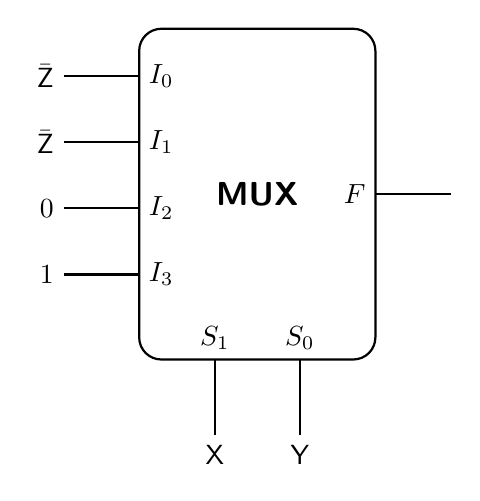
\begin{tikzpicture}[font=\sffamily, scale=1.2]
    % MUX Box
    \draw[thick, rounded corners=8pt] (0,0) rectangle (2.5,3.5);
    \node at (1.25,1.75) {\large \textbf{MUX}};

    % Left Inputs (Lines and Labels)
    % I0
    \draw[thick] (-0.8,3.0) -- (0,3.0);
    \node[left] at (-0.8,3.0) {$\bar{\text{Z}}$};
    \node[right] at (0,3.0) {$I_0$};
    
    % I1
    \draw[thick] (-0.8,2.3) -- (0,2.3);
    \node[left] at (-0.8,2.3) {$\bar{\text{Z}}$};
    \node[right] at (0,2.3) {$I_1$};
    
    % I2
    \draw[thick] (-0.8,1.6) -- (0,1.6);
    \node[left] at (-0.8,1.6) {$0$};
    \node[right] at (0,1.6) {$I_2$};
    
    % I3
    \draw[thick] (-0.8,0.9) -- (0,0.9);
    \node[left] at (-0.8,0.9) {$1$};
    \node[right] at (0,0.9) {$I_3$};

    % Bottom Select Lines
    % S1 / X
    \draw[thick] (0.8,-0.8) -- (0.8,0);
    \node[above] at (0.8,0) {$S_1$};
    \node[below] at (0.8,-0.8) {X};
    
    % S0 / Y
    \draw[thick] (1.7,-0.8) -- (1.7,0);
    \node[above] at (1.7,0) {$S_0$};
    \node[below] at (1.7,-0.8) {Y};

    % Right Output Line
    \draw[thick] (2.5,1.75) -- (3.3,1.75);
    \node[left] at (2.5,1.75) {$F$};

\end{tikzpicture}
\end{center}

\mk{12} \yr{CSE 205 | L-2/T-1 | 2021--22}

%% -- Q17: Implement F(A,B,C,D) with 4x1 MUX (2022-23) --
\item Implement the following Boolean function with a $4 \times 1$ multiplexer and external gates:
\[ F(A, B, C, D) = \Sigma\,(1, 2, 4, 7, 8, 9, 10, 11, 13, 15) \]
\mk{13} \yr{CSE 205 | L-2/T-1 | 2022--23}

%% -- Q18: Full adder using NOT gates and two 4-to-1 MUXes (2023-24) --
\item Design a full adder using NOT gates and two 4 to 1 multiplexers.
\mk{12} \yr{CSE 205 | L-2/T-1 | 2023--24}

%% -- Q19: Smart grid switching circuit 4x4 with 3-bit selector (2024-25) --
\item There is a 4$\times$4 smart grid to serve as the electricity transmission facility. The grids will be activated based on the logic function $g(a,b,c,d) = \Sigma\,(1,2,5,7,12,14)$. Design the logic circuit using a switching circuit that has 3-bit selector bits $S_2, S_1, S_0$ to select any of the eight input lines. The switching circuit is activated by two Enables — one active low $\overline{EN_0}$ and another active high $EN_1$. (Design with the minimum number of extra logic gates if required.)
\mk{13} \yr{CSE 205 | L-2/T-1 | 2024--25}

%% -- Q20: 32x1 MUX using circuit from Q5(a) (2024-25) --
\item Using the switching circuit defined above (5-bit selector lines $A, B, C, D, E$ where $A$ is MSB and $E$ is LSB), design a $32\times1$ multiplexer. (Design with the minimum number of logic gates if required.)
\mk{10} \yr{CSE 205 | L-2/T-1 | 2024--25}

\end{enumerate}

%%──────────────────────────────────────────────────────────────────────
\subtopic{cD}{Custom Combinational Circuit Design}
\label{sub:s4-comb-custom}

\begin{enumerate}

%% -- Q1: 3-input 3-output circuit (input 0-3: output+2, input 4-7: output-3) --
\item Design a combinational circuit with 3 inputs $x$, $y$, $z$ and 3 outputs $A$, $B$, $C$. When the binary input is 0, 1, 2, or 3, the binary output is two greater than the input. When the binary input is 4, 5, 6, or 7, the binary output is three less than the input.
\mk{18} \yr{CSE 205 | L-2/T-1 | 2014--15}


%% -- Q2: Binary-to-Excess-3 converter using MUX-like logic block (2016-17) --
\item Design a Binary-to-Excess-3 converter using a logic circuit block with inputs $A$, $B$, $C$, $D$, control lines $x_1$, $x_0$, and active-low $\overline{EN}$. Output~$Y$: if $x_1x_0=00$, $A \to Y$; if $01$, $B \to Y$; if $10$, $C \to Y$; if $11$, $D \to Y$.

\begin{center}
  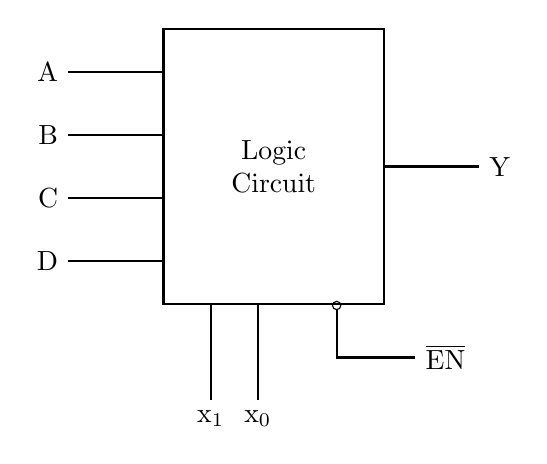
\begin{tikzpicture}[>=latex, font=\normalsize]

  % কেন্দ্রবিন্দু লজিক বক্স (Logic Circuit Box)
  \node [draw, rectangle, minimum height=3.5cm, minimum width=2.8cm, align=center, thick] (box) {
    Logic \\ Circuit
  };

  % --- ইনপুটসমূহ (বাম পাশে) ---
  % বাম ফেসের সাথে কানেকশন পয়েন্টগুলো ডিফাইন করা
  \coordinate (in1) at ([yshift=1.2cm]box.west);
  \coordinate (in2) at ([yshift=0.4cm]box.west);
  \coordinate (in3) at ([yshift=-0.4cm]box.west);
  \coordinate (in4) at ([yshift=-1.2cm]box.west);
  
  % ইনপুট টেক্সট নোট বসানো এবং তার টানা
  \node (A) [left=1.2cm of in1, anchor=east] {A}; \draw [thick] (A.east) -- (in1);
  \node (B) [left=1.2cm of in2, anchor=east] {B}; \draw [thick] (B.east) -- (in2);
  \node (C) [left=1.2cm of in3, anchor=east] {C}; \draw [thick] (C.east) -- (in3);
  \node (D) [left=1.2cm of in4, anchor=east] {D}; \draw [thick] (D.east) -- (in4);

  % --- আউটপুট (ডান পাশে) ---
  \node (Y) [right=1.2cm of box.east, anchor=west] {Y};
  \draw [thick] (box.east) -- (Y.west);

  % --- সিলেক্ট ইনপুটসমূহ (নিচে বাম পাশে) ---
  \coordinate (sel1) at ([xshift=-0.8cm]box.south);
  \coordinate (sel0) at ([xshift=-0.2cm]box.south);
  
  \draw [thick] (sel1) -- ++(0, -1.2cm) node [below] {x\textsubscript{1}};
  \draw [thick] (sel0) -- ++(0, -1.2cm) node [below] {x\textsubscript{0}};

  % --- এনেবল ইনপুট (নিচে ডান পাশে, একটিভ লো বাবল সহ) ---
  % বাবলটি (ছোট বৃত্ত) ঠিক নিচের লাইনের উপর বসানো
  \node [draw, circle, inner sep=0pt, minimum size=3pt] (bubble) at ([xshift=0.8cm]box.south) {};
  
  % বাবল থেকে তার টানা এবং এনেবল লেবেল বসানো
  \draw [thick] (bubble.south) |- ++(1.0cm, -0.6cm) node [right] {$\overline{\text{EN}}$};

\end{tikzpicture}
\end{center}

\mk{8} \yr{CSE 205 | L-2/T-1 | 2016--17}

%% -- Q3: 4-bit adder + XOR gate: A+1, A', A'+1, A based on 2-bit input (2018-19) --
\item Using a 4-bit binary adder and XOR gates, design a circuit which takes two 4-bit BCD inputs $A$ and $B$ and returns: $A+1$ if input is 00; $A'$ if input is 01; $A'+1$ if input is 10; $A$ if input is 11.
\mk{13} \yr{CSE 205 | L-2/T-1 | 2018--19}

\end{enumerate}

%%──────────────────────────────────────────────────────────────────────
\subtopic{cD}{Magnitude Comparator}
\label{sub:s4-comparator}

\begin{enumerate}

%% -- Q1: 2-bit magnitude comparator (2016-17) --
\item Design and explain a 2-bit magnitude comparator.
\mk{10} \yr{CSE 205 | L-2/T-1 | 2016--17}

%% -- Q2: Circuit returning smaller of two 4-bit numbers (2018-19) --
\item Design a logic circuit which returns the smaller value between two 4-bit binary numbers $A$ and $B$. Show the operation with $A=7$, $B=9$.
\mk{12} \yr{CSE 205 | L-2/T-1 | 2018--19}

%% -- Q3: Circuit returning maximum of two 3-bit numbers (2017-18) --
\item Design a digital circuit with logic gates which takes two 3-bit binary numbers $X$ and $Y$ and returns a 3-bit binary number $Z$ equal to the maximum between $X$ and $Y$. 
($X$ can be expressed as $X_2X_1X_0$, $Y$ can be expressed as $Y_2XY_1Y_0$; and Z can be
expressed as $Z_2Z_1Z_0$).
\mk{10} \yr{CSE 205 | L-2/T-1 | 2017--18}

%% -- Q4: Maximum of two 3-bit numbers, example 7 and 3 (2020-21) --
\item Design a logic circuit which finds the maximum value between two 3-bit numbers. Explain the operation using the two numbers 7 and 3.
\mk{10} \yr{CSE 205 | L-2/T-1 | 2020--21}

\end{enumerate}


%% ══════════════════════════════════════════════════════════════════════
%%  SECTION 5: FLIP-FLOPS, LATCHES & RACE-AROUND PROBLEMS
%% ══════════════════════════════════════════════════════════════════════
\secdivider{Flip-Flops, Latches \& Race-Around Problems}{SR, JK, D, T Flip-Flops, Excitation Tables, Race Conditions}{cE}{orange}

\markboth{S5: Flip-Flops, Latches \& Race-Around Problems}{S5: Flip-Flops, Latches \& Race-Around Problems}
\label{sec:S5}
\titleformat{\section}{\large\bfseries\color{cE}}{}{0em}{}[\titlerule]
\section*{S5 \quad Flip-Flops, Latches \& Race-Around Problems}
\addcontentsline{toc}{section}{S5: Flip-Flops, Latches \& Race-Around Problems}

%%──────────────────────────────────────────────────────────────────────
\subtopic{cE}{SR Latch \& SR/JK Undefined Condition}
\label{sub:s5-sr}

\begin{enumerate}

%% -- Q1: SR latch logic diagram and function table --
\item Show the logic diagram and function table of an SR latch with NAND gates.
\mk{4} \yr{CSE 205 | L-2/T-1 | 2011--12}

%% -- Q2: Undefined condition in SR and its JK solution --
\item Explain the undefined condition in SR flip-flops. How is this problem solved in JK flip-flops?
\mk{4+4} \yr{CSE 205 | L-2/T-1 | 2012--13}


%% -- Q3: Contact bounce elimination with S'R' latch --
\item What do you understand by mechanical switch contact bounce? Describe how the $\overline{S}\,\overline{R}$ latch can eliminate mechanical switch contact bounce.
\mk{10} \yr{CSE 205 | L-2/T-1 | 2014--15}


%% -- Q4: Excitation table for SR latch (NOR gates) --
\item Write the excitation table for a SR latch constructed with NOR gates.
\mk{4} \yr{CSE 205 | L-2/T-1 | 2015--16}

\item Consider the following transition table:

\begin{center}
\renewcommand{\arraystretch}{1.5}
\begin{tabular}{c|c|c|c|c|}
\multicolumn{1}{c}{$y \setminus x_1x_2$} & \multicolumn{1}{c}{00} & \multicolumn{1}{c}{01} & \multicolumn{1}{c}{11} & \multicolumn{1}{c}{10} \\ 
\cline{2-5}
0 & \circled{0} & \circled{0} & 1 & \circled{0} \\ 
\cline{2-5}
1 & 0 & \circled{1} & \circled{1} & \circled{1} \\ 
\cline{2-5}
\end{tabular}
\end{center}

Design the circuit with NAND SR latches and gates.
\mk{10} \yr{CSE 205 | L-2/T-1 | 2016--17}


%% -- Q5: Why S=R=1 leads to unstable condition for SR latch --
\item Discuss why the condition $S = R = 1$ leads to an unstable condition for an SR latch.
\mk{7} \yr{CSE 205 | L-2/T-1 | 2018--19}

\end{enumerate}

%%──────────────────────────────────────────────────────────────────────
\subtopic{cE}{JK Flip-Flop Characteristics}
\label{sub:s5-jk}

\begin{enumerate}

%% -- Q1: JK characteristic table and equation --
\item Derive the characteristic table and the characteristic equation for a JK flip-flop.
\mk{4} \yr{CSE 205 | L-2/T-1 | 2011--12}

%% -- Q2: Problem in construction of JK FF and its solution --
\item What is the problem in the construction of a JK flip-flop? How can we overcome this problem?
\mk{6} \yr{CSE 205 | L-2/T-1 | 2023--24}

\end{enumerate}

%%──────────────────────────────────────────────────────────────────────
\subtopic{cE}{Master-Slave D Flip-Flop}
\label{sub:s5-master-slave}

\begin{enumerate}

%% -- Q1: Master-Slave D flip-flop operation --
\item Draw and explain the operation of a Master-Slave D flip-flop.
\mk{12} \yr{CSE 205 | L-2/T-1 | 2011--12}


%% -- Q2: Block diagram and operation of master-slave negative-edge D FF --
\item Draw the block diagram and explain the operation of a Master-Slave negative edge triggered D flip-flop.
\mk{12} \yr{CSE 205 | L-2/T-1 | 2015--16}


%% -- Q3: Why use master-slave flip-flops? --
\item Why do we use master-slave flip-flops?
\mk{5} \yr{CSE 205 | L-2/T-1 | 2017--18}


%% -- Q4: Master-slave JK FF circuit using NAND gates only --
\item Draw the circuit diagram of a master-slave JK Flip-Flop using only NAND gates.
\mk{8} \yr{CSE 205 | L-2/T-1 | 2018--19}

%% -- Q5: Master-slave JK FF with async preset and clear using NOR gates (2021-22) --
\item Draw the circuit diagram of a master-slave JK flip-flop with asynchronous preset and clear using only NOR gates.
\mk{5} \yr{CSE 205 | L-2/T-1 | 2021--22}

%% -- Q6: Negative edge triggered Master-Slave D FF using D latches (2022-23) --
\item Draw the block diagram of a negative edge triggered Master-Slave D flip-flop using D latches.
\mk{10} \yr{CSE 205 | L-2/T-1 | 2022--23}

%% -- Q7: Master-slave configuration; signal propagation and race-around (2024-25) --
\item A clocked sequential circuit uses a master-slave configuration.
\begin{enumerate}
  \item Explain how signal propagation through the master and slave stages affects the timing behavior of the circuit.
  \item Analyze and justify the possibility of race-around under non-ideal clock conditions (finite rise and fall time).
\end{enumerate}
\mk{12} \yr{CSE 205 | L-2/T-1 | 2024--25}

\end{enumerate}

%%──────────────────────────────────────────────────────────────────────
\subtopic{cE}{Sequential Circuit Timing Analysis}
\label{sub:s5-timing}

\begin{enumerate}

%% -- Q1: Hold time and CLK unchanged -- Q and Q' values --
\item Consider a sequential circuit. Let the current values be: $\mathrm{CLK}=1$, $D=1$, $Q=1$, $Q'=0$. If the value of $D$ changes from 1 to 0 after the ``Hold Time'' ends and CLK remains unchanged at~1, what will be the values of $Q$ and $Q'$?

\begin{center}
  \begin{tikzpicture}[>=latex, circuitikz/nand/.style={nand port, scale=1.1}]

    % ================= গেইটগুলো বসানো (Gates) =================
    % বাম দিকের ৪টি গেইট (U1 থেকে U4)
    \node[nand port, number inputs=2] (U1) at (0, 4) {};
    \node[nand port, number inputs=2] (U2) at (0, 1.5) {};
    \node[nand port, number inputs=3] (U3) at (0, -1.5) {};
    \node[nand port, number inputs=2] (U4) at (0, -4) {};

    % ডান দিকের আউটপুট ল্যাচ গেইট (U5 ও U6)
    \node[nand port, number inputs=2] (U5) at (4.5, 1.5) {};
    \node[nand port, number inputs=2] (U6) at (4.5, -1.5) {};

    % ================= ইনপুট ও আউটপুট টেক্সট =================
    \node[left] (CLK) at (-6, 0) {$CLK$};
    \node[left] (D)   at (-4, -4.28) {$D$}; 

    \node[right] (Q) at (6, 1.5) {$Q$};
    \node[right] (Qbar) at (6, -1.5) {$\overline{Q}$};

    % ================= কানেকশন (Wiring) =================

    % CLK সিগন্যাল
    \draw (CLK) -- (-4, 0) node[circ](clk_split){} |- (U2.in 2);
    \draw (clk_split) |- (U3.in 2);

    % D সিগন্যাল
    \draw (D) -- (U4.in 2);

    % U1 এর আউটপুট থেকে U2 এর টপ ইনপুট
    \draw (U1.out) -- ++(0.2,0) -- (U2.in 1);

    % U2 এর আউটপুট এবং এর ফিডব্যাক ব্রাঞ্চগুলো
    \draw (U2.out) -- (U5.in 1);
    \draw (U2.out) -- ++(0, 1) -| ([xshift=-1cm]U1.in 1) -- (U1.in 1);
    \draw (U2.out) -- ++(0, -0.8) -| ([xshift=-1cm]U3.in 1) -- (U3.in 1);

    % U3 এর আউটপুট এবং এর ফিডব্যাক ব্রাঞ্চগুলো
    \draw (U3.out) -- (U6.in 2);
    \draw (U3.out) -- ++(0, -1) -| ([xshift=-1.2cm]U4.in 1) -- (U4.in 1);

    % U4 এর আউটপুট এবং এর ফিডব্যাক ব্রাঞ্চগুলো
    \draw (U4.out) -- ++(0.8,0) node[circ](u4_out){};
    \draw (u4_out) -- ++(0, 0.8) -| ([xshift=-1.4cm]U3.in 3) -- (U3.in 3);
    \draw (U1.in 2) -- (-3.5 , 3.75) --( -3.5, -5.5 ) -- ( 0.97, -5.5 ) -- (0.97, -4);
    % U5 এবং U6 এর আউটপুট ল্যাচ ক্রস-কাপলিং
    \draw (U5.out) -- ++(0.5,0) node[circ](q_split){} -- (Q);
    \draw (U6.out) -- ++(0.5,0) node[circ](qbar_split){} -- (Qbar);

    \draw (q_split) -- ++(0, -1.2) -| ([xshift=-0.5cm]U6.in 1) -- (U6.in 1);
    \draw (qbar_split) -- ++(0, 1.2) -| ([xshift=-0.7cm]U5.in 2) -- (U5.in 2);

\end{tikzpicture}
\end{center}

\mk{6} \yr{CSE 205 | L-2/T-1 | 2015--16}


\end{enumerate}

%%──────────────────────────────────────────────────────────────────────
\subtopic{cE}{Latch vs Flip-Flop}
\label{sub:s5-latch-ff}

\begin{enumerate}

%% -- Q1: Differences between latch and flip-flop --
\item Write the differences between a latch and a flip-flop.
\mk{5} \yr{CSE 205 | L-2/T-1 | 2013--14}

\end{enumerate}

%%──────────────────────────────────────────────────────────────────────
\subtopic{cE}{Flip-Flop Conversion}
\label{sub:s5-conversion}

\begin{enumerate}

%% -- Q1: D to T conversion --
\item Convert a D flip-flop to a T flip-flop. Use necessary gates.
\mk{4} \yr{CSE 205 | L-2/T-1 | 2011--12}

%% -- Q2: T to JK and JK to T --
\item Convert a T flip-flop into a JK flip-flop and vice versa.
\mk{4+4} \yr{CSE 205 | L-2/T-1 | 2012--13}

%% -- Q3: JK to T and D to JK --
\item Convert: (i) a JK flip-flop into a T flip-flop, and (ii) a D flip-flop into a JK flip-flop.
\mk{8} \yr{CSE 205 | L-2/T-1 | 2013--14}


%% -- Q3: SR FF using D FF and 4x1 MUX --
\item Design a SR Flip-Flop using a D Flip-Flop and a $4\times1$ MUX.
\mk{10} \yr{CSE 205 | L-2/T-1 | 2014--15}


%% -- Q4: JK FF using T FF and basic gates --
\item Design a JK Flip-Flop using a T Flip-Flop and basic gates.
\mk{10} \yr{CSE 205 | L-2/T-1 | 2016--17}


%% -- Q5: D flip-flop using T flip-flop and gates (2020-21) --
\item Design a D flip-flop using a T flip-flop and gates.
\mk{5} \yr{CSE 205 | L-2/T-1 | 2020--21}
\variant{2019--20}

%% -- Q6: JK FF from T FF; show all steps (2022-23) --
\item Construct a JK flip-flop from a T flip-flop and necessary gates. Show all the steps of this construction process.
\mk{11} \yr{CSE 205 | L-2/T-1 | 2022--23}

%% -- Q7: T flip-flop using JK FF; verify with state transitions (2024-25) --
\item Design a T flip-flop using a JK flip-flop and verify its operation using state transitions.
\mk{10} \yr{CSE 205 | L-2/T-1 | 2024--25}

%% -- Q8(b): Construct JK FF using T FF and basic gates --
\item Construct a JK flip-flop using a T flip-flop and basic gates.
\mk{6} \yr{CSE 205 | L-2/T-1 | 2023--24}

\end{enumerate}


%% ══════════════════════════════════════════════════════════════════════
%%  SECTION 6: SEQUENTIAL CIRCUITS, STATE DIAGRAMS & FSM
%% ══════════════════════════════════════════════════════════════════════
\secdivider{Sequential Circuits, State Diagrams \& FSM}{Mealy \& Moore Machines, State Tables, State Minimization, Pulse/Fundamental Mode}{cF}{teal}

\markboth{S6: Sequential Circuits, State Diagrams \& FSM}{S6: Sequential Circuits, State Diagrams \& FSM}
\label{sec:S6}
\titleformat{\section}{\large\bfseries\color{cF}}{}{0em}{}[\titlerule]
\section*{S6 \quad Sequential Circuits, State Diagrams \& FSM}
\addcontentsline{toc}{section}{S6: Sequential Circuits, State Diagrams \& FSM}

%%──────────────────────────────────────────────────────────────────────
\subtopic{cF}{State Diagram Derivation from Circuit}
\label{sub:s6-state-derivation}

\begin{enumerate}

%% -- Q1: Derive state diagram from given circuit --
\item Derive the state diagram from the following sequential circuit.
\mk{15} \yr{CSE 205 | L-2/T-1 | 2012--13}

\begin{center}
\begin{circuitikz}[scale=0.9, transform shape]
        
        % ----------------------------------------------------
        % Define components and their coordinates
        % ----------------------------------------------------
        \coordinate (x_in) at (0, 3);
        \node[not port] (not1) at (2.5, 3) {};
        \node[and port] (and1) at (4.5, 6.5) {};
        \node[or port]  (or1)  at (4.5, -0.5) {};
        \node[and port] (and2) at (10, 8) {};
        
        % ----------------------------------------------------
        % Top Flip-Flop (FF1)
        % ----------------------------------------------------
        \draw[thick] (6, 4) rectangle (8, 7);
        \node[right] at (6, 6.5) {$J_1$};
        \node[right] at (6, 4.5) {$K_1$};
        \node[right] at (6.2, 5.5) {$C$};
        \node[left]  at (8, 6.5) {$Q$};
        \node[left]  at (8, 4.5) {$\bar{Q}$};
        
        % Clock bubble and triangle for FF1
        \draw (5.8, 5.5) -- (5.9, 5.5);
        \draw (5.95, 5.5) circle(0.05); % bubble
        \draw (6, 5.35) -- (6.2, 5.5) -- (6, 5.65); % triangle
        
        % ----------------------------------------------------
        % Bottom Flip-Flop (FF2)
        % ----------------------------------------------------
        \draw[thick] (6, -1) rectangle (8, 2);
        \node[right] at (6, 1.5) {$J_2$};
        \node[right] at (6, -0.5) {$K_2$};
        \node[right] at (6.2, 0.5) {$C$};
        \node[left]  at (8, 1.5) {$Q$};
        \node[left]  at (8, -0.5) {$\bar{Q}$};
        
        % Clock bubble and triangle for FF2
        \draw (5.8, 0.5) -- (5.9, 0.5);
        \draw (5.95, 0.5) circle(0.05); % bubble
        \draw (6, 0.35) -- (6.2, 0.5) -- (6, 0.65); % triangle
        
        % ----------------------------------------------------
        % Wiring
        % ----------------------------------------------------
        
        % Input x wiring
        \draw (x_in) node[left] {$x$} -- (not1.in);
        \coordinate (x_tap_up) at (1, 3);
        \coordinate (x_tap_down) at (1.5, 3);
        
        \draw (x_tap_up) node[circ]{} |- (and1.in 1);
        \draw (x_tap_down) node[circ]{} |- (6, 1.5); % Connects to J2
        
        % NOT gate wiring (x')
        \coordinate (not_tap) at (3.5, 3);
        \draw (not1.out) -- (not_tap);
        \draw (not_tap) node[circ]{} |- (6, 4.5); % Connects to K1
        \draw (not_tap) node[circ]{} |-(3.5 , 2) |- (2.5, 2)  |- (or1.in 1); % Connects to OR1
        
        % AND1 output wiring
        \draw (and1.out) -- (6, 6.5); % Connects to J1
        \coordinate (and1_tap) at (5, 6.5);
        \draw (and1_tap) node[circ]{} |- (and2.in 1); % Connects to Output AND
        
        % OR1 output wiring
        \draw (or1.out) -- (6, -0.5); % Connects to K2
        
        % FF1 Output wiring (y1 and y1_bar)
        \draw (8, 6.5) -- (9, 6.5) node[right] {$y_1$};
        \coordinate (y1_tap) at (8.5, 6.5);
        \draw (y1_tap) node[circ]{} |- (and2.in 2);
        
        \draw (8, 4.5) -- (10, 4.5) node[right] {$\bar{y}_1$};
        \coordinate (y1bar_tap) at (10, 4.5);
        \draw (y1bar_tap) node[circ]{} |- (3, -2) |- (or1.in 2); % Feedback to OR1
        
        % FF2 Output wiring (y2 and y2_bar)
        \draw (8, 1.5) -- (9, 1.5) node[right] {$y_2$};
        \coordinate (y2_tap) at (9, 1.5);
        \draw (y2_tap) node[circ]{} |- (3, 3.5) |- (and1.in 2); % Feedback to Top AND1
        
        \draw (8, -0.5) -- (9, -0.5) node[right] {$\bar{y}_2$};
        
        % Final Output z wiring
        \draw (and2.out) -- (11, 8) node[right] {$z$};
        
        % Global Clock Line
        \draw (5.5, -2.5) node[below] {Clock} -- (5.5, 6);
        \draw (5.5, 5.5) node[circ]{} -- (5.8, 5.5);
        \draw (5.5, 0.5) node[circ]{} -- (5.8, 0.5);
        
    \end{circuitikz}
\end{center}

%% -- Q2: JK FF circuit analysis -- state table, state equations --
\item A sequential circuit has two JK Flip-Flops $A$ and $B$, two inputs $x$ and $y$, and one output $z$. The Flip-Flop input equations and circuit output equation are:
\[
  J_A = Bx + B'y',\quad K_A = B'xy',\quad J_B = A'x,\quad K_B = A + xy',\quad z = Ax'y' + Bx'y'
\]
Draw the logic diagram of the circuit, tabulate the state table and derive the state equations for $A$ and $B$.
\mk{15} \yr{CSE 205 | L-2/T-1 | 2014--15}


%% -- Q3: JK FF sequential circuit -- logic diagram, state table, state diagram (2016-17) --
\item A sequential circuit has two JK Flip-Flops $A$ and $B$, two inputs $x$ and $y$, and one output $z$. The flip-flop input equations and circuit output equation are:
\begin{align*}
  J_A &= Ax + By,\quad & K_A &= AB + xy \\
  J_B &= Ax,\quad & K_B &= ABx + By,\quad & z &= Axy + Bxy
\end{align*}
\begin{enumerate}
  \item Draw the logic diagram of the circuit.
  \item Derive the state table.
  \item Draw the state diagram.
  \end{enumerate}
\mk{4+7+4} \yr{CSE 205 | L-2/T-1 | 2016--17}

%% -- Q4: Sequential circuit with JK+T FF; logic diagram, transition/excitation/state table, state diagram (2019-20) --
\item A sequential circuit has two flip-flops $A$ and $B$, two inputs $x_1$ and $x_2$, and one output $z$. The flip-flop input equations and circuit output equations are:
\begin{align*}
  J_A &= y_A x_1 + y_B x_2,\quad  & K_A &= y_A y_B + x_1 x_2 \\
  J_B &= y_A x_1,\quad             & K_B &= y_A y_B x_1 + y_B x_2 \\
  z   &= y_A x_1 x_2 + y_B x_1 x_2
\end{align*}

For the above circuit:
\begin{enumerate}
  \item Draw the logic diagram of the circuit.
  \item Derive the transition table, excitation table, and state table.
  \item Draw the state diagram.
\end{enumerate}
\mk{25} \yr{CSE 205 | L-2/T-1 | 2019--20}

%% -- Q5: Sequential circuit with two JK FFs, two inputs, one output (2021-22) --
\item A sequential circuit has two flip-flops $A$ and $B$, two inputs $x_1$ and $x_2$, and one output $z$. The flip-flop input equations and circuit output equations are:
\begin{align*}
  J_A &= y_A x_1 + y_B x_2,\quad  & K_A &= y_A y_B + x_1 x_2 \\
  J_B &= y_A x_1,\quad             & K_B &= y_A y_B x_1 + y_B x_2 \\
  z   &= y_A x_1 x_2 + y_B x_1 x_2
\end{align*}
\begin{enumerate}
  \item Draw the logic diagram of the circuit.
  \item Derive the transition table, excitation table and state table.
  \item Draw the state diagram.
\end{enumerate}
\mk{20} \yr{CSE 205 | L-2/T-1 | 2021--22}

%% -- Q7(b): Analyze sequential circuit; transition, excitation, state table (figure-based) --
\item Analyze the sequential circuit in the figure below. Derive the transition table, excitation table and state table.

\begin{center}
      \begin{circuitikz}[thick, scale=0.9, transform shape]
        
        % T Flip-Flop
        \draw (2, 2) rectangle (4, 5);
        \node at (2.4, 4.2) {T};
        \node at (3.6, 4.2) {Q};
        \node at (3.6, 2.8) {Q'};
        \draw (2, 2.5) -- (2.2, 2.7) -- (2, 2.9); % Clock triangle
        \node[above right] at (4, 4.2) {$Q_1$};
        
        % JK Flip-Flop
        \draw (10, 2) rectangle (12, 5);
        \node at (10.4, 4.2) {J};
        \node at (10.4, 2.8) {K};
        \node at (11.6, 4.2) {Q};
        \node at (11.6, 2.8) {Q'};
        \node[above right] at (12, 4.4) {$Q_0$};
        
        % Logic Gates 
        \node[and port] (AND) at (7.5, 4.2) {};
        \node[or port]  (OR1) at (7.5, 2.8) {};
        \node[or port]  (OR2) at (14.5, 4.8) {};
        
        % Input connections
        \draw (0, 4.2) node[left] {$x$} -- (2, 4.2);
        \draw (0, 2.7) node[left] {$clk$} -- (1, 2.7);
        \draw (1, 2.7) -- (2, 2.7);
        
        % Clock routing to JK Flip-Flop (bottom line)
        \draw[fill=black] (1, 2.7) circle (0.05);
        \draw (10.4, 2) -- (10.6, 2.2) -- (10.8, 2); % Clock triangle
        \draw (1, 2.7) -- (1, 1.2) -- (10.6, 1.2) -- (10.6, 2);
        
        % Q1 connections
        \draw (4, 4.2) -- (5, 4.2);
        \draw (5, 4.2) |- (AND.in 1);
        
        % Q1 top routing to Output OR gate
        \draw (5, 4.2) -- (5, 6.0) -- (13, 6.0) |- (OR2.in 1);
        
        % Q'1 connections
        \draw (4, 2.8) |- (OR1.in 1);
        
        % Gate outputs to JK Flip-Flop
        \draw (AND.out) |- (10, 4.2);
        \draw (OR1.out) |- (10, 2.8);
        
        % Q0 connections
        \draw (12, 4.2) -- (12.5, 4.2);
        \draw[fill=black] (12.5, 4.2) circle (0.05);
        \draw (12.5, 4.2) |- (OR2.in 2);
        
        % Q0 feedback to AND gate

        \draw (6,2.9) .. controls (5.7,3) and (5.7, 3.2) .. (6,3.3);

        \draw (6,2.9) -- (6,2.5);
        \draw (6, 3.3) -- (AND.in 2);
        
        % Q'0 feedback to first OR gate
        \draw (12, 2.8) -- (13, 2.8) -- (13, 0.5) -- (6, 0.5) -- (6, 1.0);
        
        % Wire Jump (Semi-circle) over the clock line
        \draw (6, 1.0) .. controls (5.7, 1.1) and (5.7, 1.3) .. (6, 1.4);
        \draw (6, 1.4) |- (OR1.in 2);
        
        % Final Output y
        \draw (OR2.out) -- (15.5, 4.8) node[right] {$y$};
                
    \end{circuitikz}
\end{center}

\mk{12}  \yr{CSE 205 | L-2/T-1 | 2023--24}

\end{enumerate}
\label{sub:s6-circuit-design}

\begin{enumerate}

%% -- Q1: Design circuit from state diagram using T flip-flops --
\item Design the circuit corresponding to the given state diagram using T flip-flops:
\begin{enumerate}
  \item Write the state table.
  \item Find the input equations for the T flip-flops.
  \item Draw the circuit diagram.

\end{enumerate}

\begin{center}
  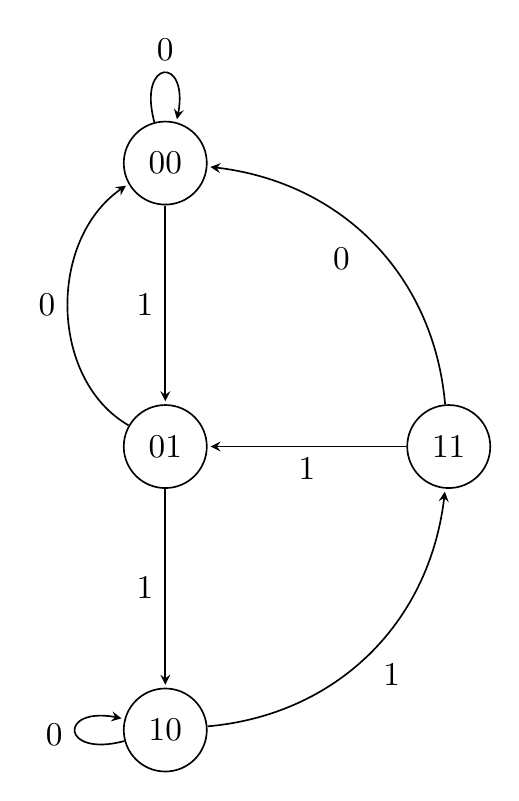
\begin{tikzpicture}[%
    >=stealth,          % তীর চিহ্নের স্টাইল
    shorten >=1pt,      % তীরে সামান্য ফাঁকা জায়গা
    auto,               % লেবেল অটোমেটিক পজিশন
    node distance=2.5cm,% নোডের মাঝের দূরত্ব
    semithick,          % তারের পুরুত্ব
    scale=1.2,          % পুরো ছবির স্কেল
    transform shape     % টেক্সটকেও স্কেল করার জন্য
]

    % ==========================================
    % 1. States (Nodes) - পজিশন সেট করা
    % ==========================================
    \node[state] (n00) at (0, 4) {00};
    \node[state] (n01) at (0, 1) {01};
    \node[state] (n11) at (3, 1) {11};
    \node[state] (n10) at (0, -2) {10};

    % ==========================================
    % 2. Transitions (Edges) - সংযোগ এবং লেবেল
    % ==========================================
    \path[->] 
        % --- Node 00 ---
        % Self-loop with label '0' above
        (n00) edge[loop above] node[black] {0} (n00)
        % Straight edge to 01 with label '1'
        (n00) edge node[black, left] {1} (n01)
        
        % --- Node 01 ---
        % Curved edge back to 00 with label '0'
        (n01) edge[bend left=60] node[black, left] {0} (n00)
        % Straight edge to 10 with label '1'
        (n01) edge node[black, left] {1} (n10)
        
        % --- Node 10 ---
        % Self-loop with label '0' below-left
        (n10) edge[loop left] node[black, left, yshift=-0.5mm] {0} (n10)
        % Curved edge up to 11 with label '1'
        (n10) edge[bend right=40] node[black, auto=right] {1} (n11)
        
        % --- Node 11 ---
        % Straight edge left to 01 with label '1' below
        (n11) edge node[black, below] {1} (n01)
        % Curved edge up-left to 00 with label '0' above
        (n11) edge[bend right=40] node[black, xshift=-1mm, yshift=0.5mm, pos=0.5] {0} (n00);

\end{tikzpicture}
\end{center}

\mk{21} \yr{CSE 205 | L-2/T-1 | 2013--14}



%% -- Q2: One-input one-output serial 2's complementer (D FF) --
\item Design a one-input, one-output serial 2's complementer using D flip-flops. The circuit accepts a string of bits from the input and generates the 2's complement at the output. The circuit can be reset asynchronously to start and end the operation. Include: (i) State diagram, (ii) State table, (iii) Simplified logic equations, (iv) Logic diagram.
\mk{15} \yr{CSE 205 | L-2/T-1 | 2015--16}


%% -- Q3: Vending machine sync circuit; 5/10/20 Tk input; JK FF (2020-21) --
\item Design a control unit with a synchronous sequential circuit for a vending machine that accepts 5\,Tk, 10\,Tk and 20\,Tk notes and releases a soft drink bottle worth 20\,Tk. The machine releases a drink whenever the deposit amount equals or exceeds 20\,Tk and keeps the change. The maximum deposit at any time is 15\,Tk. The machine releases the deposit whenever the `CHANGE' input is given. Outputs: Release Drink $Z_1$ and Release Change $Z_2$. Inputs $X_1X_2$: Tk5=00, Tk10=01, Tk20=10, CHANGE=11. Use JK Flip-Flops.
\mk{20} \yr{CSE 205 | L-2/T-1 | 2020--21}

\begin{center}
  \begin{tabular}{|c|c|}
\hline
Input & $X_1X_2$ \\
\hline
Tk 5 & 00 \\
\hline
Tk 10 & 01 \\
\hline
Tk 20 & 10 \\
\hline
CHANGE & 11 \\
\hline
\end{tabular}
\end{center}


\end{enumerate}

%%──────────────────────────────────────────────────────────────────────
\subtopic{cF}{Sequence Detector}
\label{sub:s6-sequence}

\begin{enumerate}

%% -- Q1: Three or more consecutive 1s using D flip-flops --
\item Design a sequential circuit that detects a sequence of three or more consecutive 1s in a string of bits coming through an input line. Use D flip-flops. The design must include the following:
\begin{enumerate}
  \item State diagram
  \item State table
  \item Simplified logic equations
  \item Logic 
  

  \end{enumerate}
\mk{15} \yr{CSE 205 | L-2/T-1 | 2011--12}
%% -- Q4: Sequence recognizer T FF, 4-bit non-overlapping (roll-no mod 16) (2019-20) --
\item Design a sequence recognizer using T flip-flops that recognizes a 4-bit \textbf{non-overlapping} binary sequence $X$ from an input stream of bits, where:
\[ \text{Sequence } X = \text{4-bit binary representation of your roll number} \pmod{16} \]
\mk{25} \yr{CSE 205 | L-2/T-1 | 2019--20}



%% -- Q2: Sequence detector 1010 overlapping, T FF (2016-17) --
\item Design a clocked sequential circuit that recognizes the input sequence \textbf{1010} (including overlap) such that for input $x = 01010100011010010100$ the output is $z = 00001010000001000010$. Design the circuit using T Flip-Flops and basic gates.
\mk{20} \yr{CSE 205 | L-2/T-1 | 2016--17}

%% -- Q3: Sequence recognizer 1101 overlapping, SR FF (2018-19) --
\item Design a sequence recognizer that recognizes the sequence \textbf{1101} from an input sequence (overlapping allowed). Design the circuit using SR Flip-Flops and draw the circuit diagram.
\mk{20} \yr{CSE 205 | L-2/T-1 | 2018--19}



%% -- Q2: Sequence 10011 overlapping Moore model --
\item Draw the state diagram in Moore model of a synchronous sequential circuit that results in an output of 1 whenever the sequence $10011$ occurs. The circuit is required to recognize overlapping sequences.
\mk{8} \yr{CSE 205 | L-2/T-1 | 2012--13}

%% -- Q5: Detect 3 or more consecutive 1's using D flip-flops; state diagram, table, logic eq (2022-23) --
\item Develop a sequential circuit that detects a sequence of three or more consecutive 1's in a string of bits coming through an input line. Use D flip-flops. Show the state diagram, the state table and simplified logic equations. You do not need to show the logic diagram.
\mk{12} \yr{CSE 205 | L-2/T-1 | 2022--23}

\end{enumerate}

%%──────────────────────────────────────────────────────────────────────
\subtopic{cF}{Mealy \& Moore Model Comparison \& Block Diagrams}
\label{sub:s6-mealy-moore}

\begin{enumerate}

%% -- Q1: Differentiate Mealy and Moore --
\item Differentiate Mealy and Moore models.
\mk{4} \yr{CSE 205 | L-2/T-1 | 2011--12}

%% -- Q2: Advantages and disadvantages of Mealy and Moore --
\item What are the advantages and disadvantages of using the Mealy model and the Moore model for sequential circuit design?
\mk{6} \yr{CSE 205 | L-2/T-1 | 2012--13}

%% -- Q3: Block diagrams of Mealy and Moore FSMs --
\item Draw the block diagrams of Mealy and Moore finite state machines.
\mk{6} \yr{CSE 205 | L-2/T-1 | 2013--14}


%% -- Q2: Block diagrams of Mealy and Moore machines --
\item Draw the block diagram of Mealy and Moore state machines.
\mk{8} \yr{CSE 205 | L-2/T-1 | 2015--16}


%% -- Q3: Define Mealy machine and Moore machine --
\item Define (i) a Mealy machine and (ii) a Moore machine.
\mk{5} \yr{CSE 205 | L-2/T-1 | 2017--18}


%% -- Q4: Obtain Mealy equivalent for given Moore machine (2018-19) --
\item Obtain the Mealy equivalent state table for the following Moore machine.

\begin{center}
  \begin{tabular}{|c|c|c|c|}
\hline
\multirow{2}{*}{PS} & \multicolumn{2}{c|}{NS} & \multirow{2}{*}{Z} \\ \cline{2-3}
 & x = 0 & x = 1 & \\ \hline
A & A & B & 0 \\ \hline
B & C & B & 0 \\ \hline
C & C & D & 1 \\ \hline
D & A & D & 0 \\ \hline
\end{tabular}
\end{center}

\mk{7} \yr{CSE 205 | L-2/T-1 | 2018--19}

%% -- Q5: Differentiate Mealy and Moore with block diagrams (2022-23) --
\item Differentiate between Mealy and Moore machines with block diagrams.
\mk{10} \yr{CSE 205 | L-2/T-1 | 2022--23}

%% -- Q6: Mealy/Moore block diagram with simple example (2024-25) --
\item Draw the block diagram of Mealy and Moore state machines. State the difference between two models with a simple example.
\mk{10} \yr{CSE 205 | L-2/T-1 | 2024--25}

%% -- Q7: Transform Mealy to Moore machine (2021-22) --
\item Transform the following Mealy machine into a corresponding Moore machine.

\begin{center}
  \begin{tabular}{|c|c|c|}
\hline
\multirow{2}{*}{PS} & \multicolumn{2}{c|}{NS, Z} \\ \cline{2-3} 
                    & x = 0        & x = 1        \\ \hline
A                   & C, 0         & B, 0         \\ \hline
B                   & A, 1         & D, 0         \\ \hline
C                   & B, 1         & A, 1         \\ \hline
D                   & D, 1         & C, 0         \\ \hline
\end{tabular}
\end{center}

\mk{5} \yr{CSE 205 | L-2/T-1 | 2021--22}

%% -- Q8(c): Transform Mealy machine (A-E states) into Moore machine --
\item Transform the Mealy machine shown below into a corresponding Moore machine.

\begin{center}
\begin{tabular}{|c|c|c|}
\hline
\multirow{2}{*}{PS} & \multicolumn{2}{c|}{NS, Z} \\ \cline{2-3}
 & $x=0$ & $x=1$ \\ \hline
A & B, 1 & C, 0 \\ \hline
B & C, 1 & D, 0 \\ \hline
C & D, 0 & E, 1 \\ \hline
D & E, 0 & A, 1 \\ \hline
E & A, 1 & B, 1 \\ \hline
\end{tabular}
\end{center}

\mk{6} \yr{CSE 205 | L-2/T-1 | 2023--24}

\end{enumerate}
%%──────────────────────────────────────────────────────────────────────
\subtopic{cF}{State Minimization (Implication Table)}

\label{sub:s6-state-min}

\begin{enumerate}

%% -- Q1: Implication table state reduction (A-H) --
\item Using an implication table, reduce the following state table to a minimum number of states and write the reduced state table.
\mk{17} \yr{CSE 205 | L-2/T-1 | 2012--13}

\begin{center}
  \begin{tabular}{|c|c|c|}
        \cline{2-3}
        \multicolumn{1}{c|}{} & \multicolumn{2}{c|}{\textbf{X}} \\
        \cline{2-3}
        \multicolumn{1}{c|}{} & \textbf{0} & \textbf{1} \\
        \hline
        A & E/0 & D/0 \\
        \hline
        B & A/1 & F/0 \\
        \hline
        C & C/0 & A/1 \\
        \hline
        D & B/0 & A/0 \\
        \hline
        E & D/1 & C/0 \\
        \hline
        F & C/0 & D/1 \\
        \hline
        G & H/1 & G/1 \\
        \hline
        H & C/1 & B/1 \\
        \hline
    \end{tabular}
\end{center}

\item Using an implication table, reduce the following state table to a minimum number of states and write the reduced state table.
\mk{15} \yr{CSE 205 | L-2/T-1 | 2013--14}

\begin{center}
  \begin{tabular}{|c|c|c|c|c|}
        \hline
        \multirow{2}{*}{Present State} & \multicolumn{2}{c|}{Next State} & \multicolumn{2}{c|}{Output} \\
        \cline{2-5}
         & $x = 0$ & $x = 1$ & $x = 0$ & $x = 1$ \\
        \hline
        A & F & B & 0 & 0 \\
        \hline
        B & D & C & 0 & 0 \\
        \hline
        C & F & E & 0 & 0 \\
        \hline
        D & G & A & 1 & 0 \\
        \hline
        E & D & C & 0 & 0 \\
        \hline
        F & F & B & 1 & 1 \\
        \hline
        G & G & H & 0 & 1 \\
        \hline
        H & G & A & 1 & 0 \\
        \hline
    \end{tabular}
\end{center}


%% -- Q2: Critical race-free assignment using multiple-row method --
\item Find a critical race-free state assignment for a reduced flow table (states $a$--$d$, inputs 00/01/11/10) using the Multiple-row method.

\begin{center}
  \begin{tabular}{c|c|c|c|c|}
        \multicolumn{1}{c}{} & \multicolumn{1}{c}{00} & \multicolumn{1}{c}{01} & \multicolumn{1}{c}{11} & \multicolumn{1}{c}{10} \\
        \cline{2-5}
        % Row 'a' - First and third cells are colored light gray
        $a$ & \cellcolor{gray!20}\mycircle{$a$} & $c$ & \cellcolor{gray!20}\mycircle{$a$} & $d$ \\
        \cline{2-5}
        % Row 'b' - All cells are colored light gray
        $b$ & \cellcolor{gray!20}$a$ & \cellcolor{gray!20}\mycircle{$b$} & \cellcolor{gray!20}$c$ & \cellcolor{gray!20}\mycircle{$b$} \\
        \cline{2-5}
        % Row 'c' - No background color
        $c$ & \mycircle{$c$} & \mycircle{$c$} & \mycircle{$c$} & $d$ \\
        \cline{2-5}
        % Row 'd' - No background color
        $d$ & \mycircle{$d$} & $b$ & $a$ & \mycircle{$d$} \\
        \cline{2-5}
    \end{tabular}
\end{center}

\mk{10} \yr{CSE 205 | L-2/T-1 | 2014--15}



%% -- Q3: Reduce state table using implication table (2015-16) --
\item You are given a state table of a synchronous sequential circuit. Find the reduced state table using the implication table.

\begin{center}
  \begin{tabular}{|c|c|c|c|c|}
        \hline
        \multirow{2}{*}{\begin{tabular}[c]{@{}c@{}}Present \\ State\end{tabular}} & \multicolumn{2}{c|}{Next State} & \multicolumn{2}{c|}{Output} \\ \cline{2-5} 
        & x=0 & x=1 & x=0 & x=1 \\ \hline
        a & d & b & 0 & 0 \\ \hline
        b & e & a & 0 & 0 \\ \hline
        c & g & f & 0 & 1 \\ \hline
        d & a & d & 1 & 0 \\ \hline
        e & a & d & 1 & 0 \\ \hline
        f & c & b & 0 & 0 \\ \hline
        g & a & e & 1 & 0 \\ \hline
    \end{tabular}
\end{center}

\mk{12} \yr{CSE 205 | L-2/T-1 | 2015--16}

\item You are given the following state table of a synchronous sequential circuit. 

\begin{center}
\renewcommand{\arraystretch}{1.3}
\begin{tabular}{|c|c|c|c|c|}
\hline
\multirow{2}{*}{\begin{tabular}[c]{@{}c@{}}Present\\ State\end{tabular}} & \multicolumn{2}{c|}{Next State} & \multicolumn{2}{c|}{Output} \\ \cline{2-5} 
 & $x = 0$ & $x = 1$ & $x = 0$ & $x = 1$ \\ \hline
a & a & c & 0 & 0 \\ \hline
b & d & a & 1 & 0 \\ \hline
c & f & f & 0 & 0 \\ \hline
d & e & b & 1 & 0 \\ \hline
e & g & g & 1 & 0 \\ \hline
f & c & c & 0 & 0 \\ \hline
g & b & h & 1 & 0 \\ \hline
h & h & c & 0 & 0 \\ \hline
\end{tabular}
\end{center}

\begin{enumerate}
    \item[(i)] Find the reduced state table using an implication table.
    \item[(ii)] Draw the equivalent minimized state diagram.
\end{enumerate}
\mk{10} \yr{CSE 205 | L-2/T-1 | 2016--17}


%% -- Q4: Completely specified circuit; equivalence partitions; minimal state table --
\item For the state-table of a completely specified circuit, find the equivalence partitions and write the state-table of the minimal machine. Name the states that are equivalent.
\textit{[Diagram: state table with present states $a$--$h$ and next states/outputs for $x=0$ and $x=1$ to be inserted.]}
\mk{12+3} \yr{CSE 205 | L-2/T-1 | Uncertain}

%% -- Q5: Completely specified; equivalence partitions (2017-18) --
\item For the state-table of a completely specified circuit, find the equivalence partitions and write the state-table of the minimal machine. Name the equivalent states.

\begin{center}
  \begin{tabular}{c|cccc}
\multicolumn{1}{r}{$x_1x_2$} & \multicolumn{4}{c}{NS,Z} \\
\multicolumn{1}{l}{PS} & 00 & 01 & 11 & 10 \\
\hline
A & D, 0 & D, 0 & F, 0 & A, 0 \\
B & C, 1 & D, 0 & E, 1 & F, 0 \\
C & C, 1 & D, 0 & E, 1 & A, 0 \\
D & D, 0 & B, 0 & A, 0 & F, 0 \\
E & C, 1 & F, 0 & E, 1 & A, 0 \\
F & D, 0 & D, 0 & A, 0 & F, 0 \\
G & G, 0 & G, 0 & A, 0 & A, 0 \\
H & B, 1 & D, 0 & E, 1 & A, 0 \\
\end{tabular}
\end{center}


\mk{10} \yr{CSE 205 | L-2/T-1 | 2017--18}

%% -- Q6: Completely specified; equivalence partitions (2018-19) --
\item For the state-table of a completely specified circuit, find the equivalent partitions and write the state-table of the minimal machine. Name the equivalent states.

\begin{center}
  \begin{tabular}{|c|c|c|c|}
\hline
\multirow{2}{*}{PS} & \multicolumn{3}{c|}{NS, Z} \\ \cline{2-4} 
 & I & J & K \\ \hline
A & A,0 & B,1 & E,1 \\ \hline
B & B,0 & A,1 & F,1 \\ \hline
C & A,1 & D,0 & E,0 \\ \hline
D & F,0 & C,1 & A,0 \\ \hline
E & A,0 & D,1 & E,1 \\ \hline
F & B,0 & D,1 & F,1 \\ \hline
\end{tabular}
\end{center}

\mk{8} \yr{CSE 205 | L-2/T-1 | 2018--19}

%% -- Q7: Completely specified; equivalence partitions with given table (2020-21) --
\item For the state-table of a completely specified circuit (PS: A--H), find the equivalence partitions and write the state-table of the minimal machine. Name the state that are equivalent .
\par\smallskip
\begin{center}
  
\begin{tabular}{c|cc}
\toprule
PS & NS, $Z$ ($x=0$) & NS, $Z$ ($x=1$)\\
\midrule
A & B,1 & H,1 \\ B & F,1 & D,1 \\ C & D,0 & E,1 \\ D & C,0 & F,1 \\
E & D,1 & C,1 \\ F & C,1 & C,1 \\ G & C,1 & D,1 \\ H & C,0 & A,1 \\
\bottomrule
\end{tabular}
\end{center}
\mk{10} \yr{CSE 205 | L-2/T-1 | 2020--21}

\end{enumerate}

%%──────────────────────────────────────────────────────────────────────
\subtopic{cF}{Incompletely Specified Machine Minimization}
\label{sub:s6-incomp}

\begin{enumerate}

%% -- Q1: Incompletely specified; implication table, maximal compatibles/incompatibles, bounds, minimal machine (2017-18) --
\item For the incompletely specified machine , complete the implication table and determine the maximal compatibles and maximal incompatibles. Find the upper and lower bounds on the number of states of the minimal machine. Give the state table of the minimal machine.
\begin{center}
  \begin{tabular}{c|cc}
PS & \multicolumn{2}{c}{NS,Z} \\
 & x = 0 & x = 1 \\
\hline
A & A, - & B, 1 \\
B & G, - & D, 0 \\
C & B, 1 & B, - \\
D & A, 1 & B, - \\
E & C, - & A, - \\
F & F, - & C, - \\
G & G, - & G, - \\
\end{tabular}
\end{center}
  
\mk{15} \yr{CSE 205 | L-2/T-1 | 2017--18}

%% -- Q2: Incompletely specified; same procedure (2018-19) --
\item For the incompletely specified machine (Figure 7(a)), complete the implication table and determine the maximal compatibles and maximal incompatibles. Find the upper and lower bounds. Give the state table of the minimal machine.

\begin{center}
  \begin{tabular}{|c|c|c|}
\hline
\multirow{2}{*}{PS} & \multicolumn{2}{c|}{NS, Z} \\ \cline{2-3} 
 & x = 0 & x = 1 \\ \hline
A & B, 0 & C, 1 \\ \hline
B & D, 0 & C, 1 \\ \hline
C & A, 0 & E, 0 \\ \hline
D & - & F, 1 \\ \hline
E & G, 1 & F, 0 \\ \hline
F & B, 0 & - \\ \hline
G & D, 0 & E, 0 \\ \hline
\end{tabular}
\end{center}

\mk{20} \yr{CSE 205 | L-2/T-1 | 2018--19}

%% -- Q3: Incompletely specified with given table (2020-21) --
\item For the incompletely specified machine below, complete the implication table and determine the maximal compatibles and maximal incompatibles. Find the upper and lower bounds on the number of states of the minimal machine. Give the state table of the minimal machine.
\par\smallskip
\begin{center}
  \begin{tabular}{|c|c|c|c|c|}
\hline
PS & \multicolumn{4}{c|}{NS, $Z_1Z_2$} \\
\cline{2-5}
 & 00 & 01 & 11 & 10 \\
\hline
A & A, 00 & E, 01 & - & A, 01 \\
\hline
B & - & C, 10 & B, 00 & D, 11 \\
\hline
C & A, 00 & C, 10 & - & - \\
\hline
D & A, 00 & - & - & D, 11 \\
\hline
E & - & E, 01 & F, 00 & - \\
\hline
F & - & G, 10 & F, 00 & G, 11 \\
\hline
G & A, 00 & - & - & G, 11 \\
\hline
\end{tabular}
\end{center}
\mk{25} \yr{CSE 205 | L-2/T-1 | 2020--21}


%% -- Q4: Incompletely specified machine with given table (2019-20) --
\item For the incompletely specified machine shown below, derive the implication table and determine the maximal compatibles and the maximal incompatibles. Find the upper bound and the lower bound of the minimal machine and determine the minimal machine.

\begin{center}
  \begin{tabular}{|c|c|c|}
\hline
\multirow{2}{*}{PS} & \multicolumn{2}{c|}{NS, Z} \\ \cline{2-3} 
 & x = 0 & x = 1 \\ \hline
A & A, - & B, 1 \\ \hline
B & G, - & D, 0 \\ \hline
C & B, 1 & B, - \\ \hline
D & A, 1 & B, - \\ \hline
E & C, - & A, - \\ \hline
F & F, - & C, - \\ \hline
G & G, - & G, - \\ \hline
\end{tabular}
\end{center}

\mk{25} \yr{CSE 205 | L-2/T-1 | 2019--20}

%% -- Q5: Incompletely specified machine; maximal compatibles; upper and lower bound (2021-22) --
\item For the incompletely specified machine shown in the figure, derive the implication table and determine the maximal compatibles and the maximal incompatibles. Find the upper bound and the lower bound of the number of states of the minimal machine. Give the state table of the minimal machine.

\begin{center}
  \begin{tabular}{|c|c|c|c|}
\hline
\multirow{2}{*}{PS} & \multicolumn{3}{c|}{NS, Z} \\ \cline{2-4} 
                    & $I_1$   & $I_2$   & $I_3$   \\ \hline
A                   & C, 0    & E, 1    & -       \\ \hline
B                   & C, 0    & E, -    & -       \\ \hline
C                   & B, -    & C, 0    & A, -    \\ \hline
D                   & B, 0    & C, -    & E, -    \\ \hline
E                   & -       & E, 0    & A, -    \\ \hline
\end{tabular}
\end{center}

\mk{15} \yr{CSE 205 | L-2/T-1 | 2021--22}

%% -- Q6: Reduce state table using implication table (2022-23) --
\item Reduce the number of states of the following state table using implication table. Show the reduced state table.

\begin{center}
  \begin{tabular}{|c|c|c|c|c|}
\hline
\multirow{2}{*}{State} & \multicolumn{2}{c|}{Next State} & \multicolumn{2}{c|}{Output} \\ \cline{2-5} 
                       & Input X = 0    & Input X = 1    & Input X = 0  & Input X = 1  \\ \hline
A                      & A              & B              & 0            & 0            \\ \hline
B                      & C              & D              & 0            & 1            \\ \hline
C                      & A              & B              & 0            & 0            \\ \hline
D                      & E              & D              & 0            & 1            \\ \hline
E                      & A              & D              & 0            & 1            \\ \hline
\end{tabular}
\end{center}

\mk{11} \yr{CSE 205 | L-2/T-1 | 2022--23}

%% -- Q7: Equivalence partitions; implication table; minimal machine (2024-25) --
\item For the state table of a completely specified asynchronous sequential circuit, find out the equivalent partitions, implication table. Formulate the state table of the minimal machine. Find out the states those are equivalent.

\begin{center}
  \begin{tabular}{|l|l|l|l|l|}
\hline
x1x2 & NS, z & & & \\ \hline
PS & x1x2=00 & x1x2=01 & x1x2=11 & x1x2=10 \\ \hline
A & D/0 & D/0 & F/0 & A/0 \\ \hline
B & C/1 & D/0 & E/1 & F/0 \\ \hline
C & C/1 & D/0 & E/1 & A/0 \\ \hline
D & D/0 & B/0 & A/0 & F/0 \\ \hline
E & C/1 & F/0 & E/1 & A/0 \\ \hline
F & D/0 & D/0 & A/0 & F/0 \\ \hline
G & G/0 & G/0 & A/0 & A/0 \\ \hline
H & B/1 & D/0 & E/1 & A/0 \\ \hline
\end{tabular}

\vspace{0.3cm}
(PS = Present state, NS = next state, x1, x2 are input, z is output)
\end{center}

\mk{12} \yr{CSE 205 | L-2/T-1 | 2024--25}

%% -- Q8: Incompletely specified; implication table; maximal compatibles/incompatibles; bounds; minimal machine --
\item For the incompletely specified machine shown below, derive the implication table and determine the maximal compatibles and the maximal incompatibles. Find the upper bound and the lower bound of the number of states of the minimal machine. Give the state table of the minimal machine.

\begin{center}
\begin{tabular}{|c|c|c|}
\hline
\multirow{2}{*}{PS} & \multicolumn{2}{c|}{NS, Z} \\ \cline{2-3}
 & $x=0$ & $x=1$ \\ \hline
A & B, 0 & C, 0 \\ \hline
B & D, 0 & --, -- \\ \hline
C & F, 0 & E, 1 \\ \hline
D & B, 0 & G, 0 \\ \hline
E & F, 0 & C, 1 \\ \hline
F & E, 0 & D, 1 \\ \hline
G & F, 0 & --, -- \\ \hline
\end{tabular}
\end{center}

\mk{23} \yr{CSE 205 | L-2/T-1 | 2023--24}

\end{enumerate}


%%──────────────────────────────────────────────────────────────────────
\subtopic{cF}{Redundant States}

\label{sub:s6-redundant}

\begin{enumerate}

%% -- Q1: Problems due to redundant states --
\item What are the problems that may occur when redundant states are present in the state diagram?
\mk{6} \yr{CSE 205 | L-2/T-1 | 2012--13, 2013--14}

\end{enumerate}

%%──────────────────────────────────────────────────────────────────────
\subtopic{cF}{Output Assignment in Flow Table}
\label{sub:s6-output-assign}

\begin{enumerate}

%% -- Q1: Procedure to assign output to unstable states --
\item Write down the procedure to assign the output to unstable states in a flow table.
\mk{7} \yr{CSE 205 | L-2/T-1 | 2011--12}

\end{enumerate}

%%──────────────────────────────────────────────────────────────────────
\subtopic{cF}{Fundamental Mode Design}
\label{sub:s6-fundamental}

\begin{enumerate}

%% -- Q1: Gated latch primitive and reduced flow table --
\item A specification is given below for a gated latch circuit with two inputs $G$ and $D$ and an output $Q$. Assume fundamental mode operation.

\textit{``Binary information present at the D input is transferred to the Q output when G is equal to 1. The Q output will follow the D input as long as G = 1. When G goes to 0, the information that was present at the D input at the time the transition occurred is retained at the Q output.''}

Derive the primitive flow table and then obtain the reduced flow table.
\mk{6+6} \yr{CSE 205 | L-2/T-1 | 2011--12}


%% -- Q2: Primitive flow table -- implication table, merger diagram, minimal closed set --
\item For a given primitive flow table (states $a$--$h$, inputs 00/01/11/10), perform the following:
\begin{enumerate}
  \item Find all compatible pairs by means of an implication table.
  \item Find the maximal compatibles by means of a merger diagram.
  \item Find a minimal set of compatibles that covers all the states and is closed.
\end{enumerate}

%% -- Q9: Fundamental mode electrical lock; two inputs X1, X2; lock opens Z=1 (2019-20) --
\item Design a fundamental mode circuit to function as an electrical lock. The lock has two switch inputs $X_1$ and $X_2$. Design the circuit so that the lock-open signal $Z=1$ is produced only after the following conditions have been satisfied:
\begin{enumerate}
  \item Begin with $X_1 = X_2 = 0$.
  \item While $X_2 = 0$, $X_1$ is turned on and then turned off.
  \item Then while $X_1$ remains off, $X_2$ is turned on to open the lock ($Z=1$).
  \item For any deviation in the sequence of the above transitions, the lock remains closed ($Z=0$).
\end{enumerate}
Determine the primitive flow table, reduced flow table, race-free state assignment, K-maps and circuit diagram.
\mk{25} \yr{CSE 205 | L-2/T-1 | 2019--20}


%% -- Q3: Fundamental mode definition --
\item What does it mean when an asynchronous sequential circuit is assumed to operate in the fundamental mode?
\mk{4} \yr{CSE 205 | L-2/T-1 | 2015--16}

%% -- Q4: Primitive flow table for negative-edge triggered T FF --
\item Derive the primitive flow table for a negative-edge triggered T flip-flop.
\mk{12} \yr{CSE 205 | L-2/T-1 | 2015--16}


%% -- Q5: Primitive flow table + minimum row reduction (2017-18) --
\item Construct a primitive flow table for a fundamental mode circuit with two inputs ($x_1$, $x_2$) and two outputs ($z_1$, $z_2$). Specifications: when $x_1x_2=00$, $z_1z_2=00$. Output 10 is produced following input sequence $00\to01\to11$ and remains until $x_1x_2$ returns to 00. Output 01 is produced following sequence $00\to10\to11$ and remains until 00 input returns the output to 00. Determine the minimum row-reduced flow table.
\mk{10+10} \yr{CSE 205 | L-2/T-1 | 2017--18}

%% -- Q6: Primitive flow table (2018-19) --
\item Construct a primitive flow table for a fundamental mode circuit where the output $z=0$ when the two inputs $x_1$ and $x_2$ are equal. $z=1$ results when $x_1=0$ and $x_2$ changes from 0 to 1, and when $x_1=1$ and $x_2$ changes from 1 to 0. No other input change causes any output change. Determine the reduced flow table containing the minimum number of rows.
\mk{10+10} \yr{CSE 205 | L-2/T-1 | 2018--19}

%% -- Q7: Primitive flow table (2020-21) --
\item Design a two-input ($x_1$, $x_2$), one-output ($z$) fundamental mode circuit that operates as follows. The output changes from 0 to 1 only on the first $x_1$ input change that follows an $x_2$ input change. A $1\to0$ output change occurs only when $x_1$ changes from 1 to 0 while $x_2=1$. Determine the primitive flow table, reduced flow table, race-free state assignment, K-maps and circuit diagram.
\mk{25} \yr{CSE 205 | L-2/T-1 | 2020--21}


%% -- Q8: Digital lock using T latches; sequence AABABA; 3B reset; bell output (2018-19) --
\item Design a circuit for a digital lock using T latches. The lock has two push-button inputs $A$ and $B$ and produces a single pulse $Z_1$ for each activation. The two switches are mechanically interlocked so that simultaneous pulses are not possible. Features: (i) opening sequence is AABABA; (ii) three $B$ pulses give absolute reset; (iii) any incorrect use of $A$ produces output $Z_2$ to ring a bell.
\mk{20} \yr{CSE 205 | L-2/T-1 | 2018--19}

%% -- Q9: Traffic light controller at railroad crossing; primitive flow table (2021-22) --
\item At a junction of a single-track railroad and a road, traffic lights are to be installed. The lights are to be controlled by switches that are pressed or released by the trains. When a train approaches the junction from either direction and is within 1500 feet from it, the lights are to change from green to red and remain red until the train is 1500 feet past the junction. You may assume that the length of a train is smaller than 3000 feet. Determine a primitive flow table and reduce it.
\mk{20} \yr{CSE 205 | L-2/T-1 | 2021--22}

%% -- Q10: Async circuit; 3 inputs a,b,c; output U=1 only if all=1 in order a,b,c --
\item Design an asynchronous circuit functioning in fundamental mode. The circuit has three inputs $a$, $b$, and $c$, and one output $U$. $U=1$ only if all inputs are equal to `1', and they went to `1' in the order $a$, $b$, then $c$. $U$ returns to 0 when all inputs are returned to `0'. Derive the primitive flow table, reduced flow table and the minimum number of states required to have a race-free state assignment, and find a possible state assignment.
\mk{23} \yr{CSE 205 | L-2/T-1 | 2023--24}

\end{enumerate}


%%──────────────────────────────────────────────────────────────────────
\subtopic{cF}{Excitation Function \& Transition Table}

\label{sub:s6-excitation}

\begin{enumerate}

%% -- Q1: Y = X1X2' + (X1+X2')y -- logic diagram and transition table --
\item An asynchronous sequential circuit is described by the following excitation function:
\[ Y = X_1 X_2' + (X_1 + X_2')\,y \]
Draw the logic diagram of the circuit and derive the transition table.
\mk{10} \yr{CSE 205 | L-2/T-1 | 2015--16}


%% -- Q2: Two internal states; Y1, Y2, Z from excitation functions (2016-17) --
\item An asynchronous sequential circuit has two internal states and one output. The excitation and output functions are:
\begin{align*}
  Y_1 &= x_1 x_2 + x_1 y_2' + x_2' y_1 \\
  Y_2 &= x_2 + x_1 y_1' y_2 + x_1' y_1 \\
  Z   &= x_2 + y_1
\end{align*}
Draw the logic diagram of the circuit and derive the transition table.
\mk{15} \yr{CSE 205 | L-2/T-1 | 2016--17}

%% -- Q3: Excitation Y=x1x2'+(x1+x2')y; z=y; logic diagram, transition table, flow table (2022-23) --
\item An asynchronous sequential circuit is described by the excitation function $Y = x_1x_2' + (x_1 + x_2')y$ and the output function $z = y$.
\begin{enumerate}
  \item Draw the logic diagram of the circuit.
  \item Derive the transition table and output map.
  \item Obtain a two-state flow table.
\end{enumerate}
\mk{12} \yr{CSE 205 | L-2/T-1 | 2022--23}

\end{enumerate}

%%──────────────────────────────────────────────────────────────────────
\subtopic{cF}{Hazards in Asynchronous Circuits}
\label{sub:s6-hazards}

\begin{enumerate}

%% -- Q1: Static-1 hazard definition and example --
\item What is a static-1 hazard? Give an example of a static-1 hazard in an asynchronous sequential circuit.
\mk{5} \yr{CSE 205 | L-2/T-1 | 2015--16}

\end{enumerate}

%%──────────────────────────────────────────────────────────────────────
\subtopic{cF}{Serial Parity Generation}
\label{sub:s6-parity}

\begin{enumerate}
  \item For the following primitive flow table shown in Figure , answer the following questions:
\begin{enumerate}[label=(\roman*)]
    \item Find all compatible pairs by means of an implication table.
    \item Find the maximal compatibles by means of a merger diagram.
    \item Find a minimal set of compatibles that covers all the states and is closed.
\end{enumerate}
\vspace{1.5em}

\begin{center}
\renewcommand{\arraystretch}{1.5} % টেবিলের রো-এর উচ্চতা একটু বাড়ানোর জন্য
\begin{tabular}{|c|c|c|c|c|}
\hline
\multicolumn{1}{c}{} & \multicolumn{1}{c}{00} & \multicolumn{1}{c}{01} & \multicolumn{1}{c}{11} & \multicolumn{1}{c}{10} \\ \cline{2-5}
$a$ & \circled{$a$}, $0$ & $b$, $-$ & $-$, $-$ & $e$, $-$ \\ \cline{2-5}
$b$ & $a$, $-$ & \circled{$b$}, $0$ & $c$, $-$ & $-$, $-$ \\ \cline{2-5}
$c$ & $-$, $-$ & $d$, $-$ & \circled{$c$}, $0$ & $h$, $-$ \\ \cline{2-5}
$d$ & $a$, $-$ & \circled{$d$}, $1$ & $-$, $-$ & $-$, $-$ \\ \cline{2-5}
$e$ & $a$, $-$ & $-$, $-$ & $f$, $-$ & \circled{$e$}, $0$ \\ \cline{2-5}
$f$ & $-$, $-$ & $g$, $-$ & \circled{$f$}, $0$ & $h$, $-$ \\ \cline{2-5}
$g$ & $a$, $-$ & \circled{$g$}, $0$ & $-$, $-$ & $-$, $-$ \\ \cline{2-5}
$h$ & $a$, $-$ & $-$, $-$ & $-$, $-$ & \circled{$h$}, $0$ \\ \hline
\multicolumn{5}{c}{Fig. for Q. 6 (a)}
\end{tabular}
\end{center}

\mk{10+5+5} \yr{CSE 205 | L-2/T-1 | 2014--15}

%% -- Q1: Serial parity generation circuit; 0=even, 1=odd (2018-19) --
\item Design a serial parity generation circuit. The circuit receives a sequence of bits and determines whether the sequence contains an even or odd number of ones. The output $p$ should be 0 for even parity and 1 for odd parity.
\mk{8} \yr{CSE 205 | L-2/T-1 | 2018--19}

%% -- Q2: Serial parity generation circuit (repeat 2020-21) --
\item Design a serial parity generation circuit. The circuit receives a sequence of bits and determines whether the sequence contains an even or odd number of ones. The circuit output $p$ should be 0 for even parity and 1 for odd parity.
\mk{10} \yr{CSE 205 | L-2/T-1 | 2020--21}

\end{enumerate}



%%──────────────────────────────────────────────────────────────────────
\subtopic{cF}{Race Around Condition}
\label{sub:s6-race}

\begin{enumerate}

%% -- Q1: Critical and non-critical races --
\item What is a race in fundamental mode circuits? Explain critical and non-critical races with an example.
\mk{4+8} \yr{CSE 205 | L-2/T-1 | 2011--12}


%% -- Q2: Race conditions in transition table -- critical/noncritical, cycles --
\item Investigate the transition table (state variables $y_1 y_2$, inputs $x_1 x_2$) and determine all race conditions and whether they are critical or noncritical. Determine also whether there are any cycles.

\begin{center}
  \begin{tabular}{c|c|c|c|c|}
    \multicolumn{1}{c}{} & \multicolumn{4}{c}{$x_1x_2$} \\
    \multicolumn{1}{c}{$y_1y_2$} & \multicolumn{1}{c}{00} & \multicolumn{1}{c}{01} & \multicolumn{1}{c}{11} & \multicolumn{1}{c}{10} \\
    \cline{2-5}
    00 & 10 & \mycircle{00} & 11 & 10 \\
    \cline{2-5}
    01 & \mycircle{01} & 00 & 10 & 10 \\
    \cline{2-5}
    11 & 01 & 00 & \mycircle{11} & \mycircle{11} \\
    \cline{2-5}
    10 & 11 & 00 & \mycircle{10} & \mycircle{10} \\
    \cline{2-5}
\end{tabular}
\end{center}

\mk{10} \yr{CSE 205 | L-2/T-1 | 2014--15}

\item What is race condition? Explain different types of races with examples.
\mk{10} \yr{CSE 205 | L-2/T-1 | 2016--17}


%% -- Q3: Race-free assignment from reduced flow table (2017-18) --
\item For the given reduced flow table, find a valid assignment without any critical race and complete the modified flow table.

\begin{center}
  \begin{tabular}{c|cccc}
\diagbox{}{$x_1x_2$} & 00 & 01 & 11 & 10 \\
\hline
a & \circled{a}/0 & d/0 & \circled{a}/1 & c/0 \\
b & \circled{b}/0 & c/- & \circled{b}/0 & d/- \\
c & b/0 & \circled{c}/1 & a/1 & \circled{c}/0 \\
d & a/0 & \circled{d}/0 & b/0 & \circled{d}/1 \\
\end{tabular}
\end{center}

\mk{10} \yr{CSE 205 | L-2/T-1 | 2017--18}

%% -- Q4: Race-free assignment (2018-19) --
\item For the given reduced flow table, find a valid assignment without any critical race and complete the modified flow table.

\begin{center}
  \begin{tabular}{c|cccc}
\diagbox{}{$x_1x_2$} & 00 & 01 & 11 & 10 \\
\hline
a & \circled{a}/0 & d/0 & \circled{a}/1 & c/0 \\
b & \circled{b}/0 & c/- & \circled{b}/0 & d/- \\
c & b/0 & \circled{c}/1 & a/1 & \circled{c}/0 \\
d & a/0 & \circled{d}/0 & b/0 & \circled{d}/1 \\
\end{tabular}
\end{center}

\mk{8} \yr{CSE 205 | L-2/T-1 | 2018--19}

%% -- Q5: Race-free assignment with given table (2020-21) --
\item For the given reduced flow table, find a valid assignment without any critical race and complete the modified flow table.
\par\smallskip
\begin{center}
  \begin{tabular}{c|cccc}
  \diagbox{}{ $x_1x_2$ } & 00 & 01 & 11 & 10 \\
  \hline
  a & \textcircled{a}/0 & b/- & \textcircled{a}/1 & b/- \\
  b & a/- & \textcircled{b}/0 & c/- & \textcircled{b}/0 \\
  c & a/- & \textcircled{c}/1 & \textcircled{c}/0 & b/- \\
\end{tabular}
\end{center}
\mk{10} \yr{CSE 205 | L-2/T-1 | 2020--21}

%% -- Q6: Race-free assignment from reduced flow table A-D (2021-22) --
\item For the given reduced flow table, find a valid assignment without any critical race and complete the modified flow table.

\begin{center}
  \begin{tabular}{|c|c|c|c|c|}
\hline
  & 00    & 01    & 11    & 10    \\ \hline
A & (A),0 & D,0   & B,-   & (A),0 \\ \hline
B & A,-   & -     & C,-   & -     \\ \hline
C & A,-   & (C),1 & (C),1 & (C),1 \\ \hline
D & A,0   & (D),0 & (D),0 & C,-   \\ \hline
\end{tabular}
\end{center}

\mk{10} \yr{CSE 205 | L-2/T-1 | 2021--22}

%% -- Q7: Race conditions in asynchronous circuits (2022-23) --
\item What is a race in fundamental mode circuits? Explain critical and non-critical races with examples.
\mk{12} \yr{CSE 205 | L-2/T-1 | 2022--23}

\end{enumerate}

%%──────────────────────────────────────────────────────────────────────
\subtopic{cF}{Pulse Mode Logic}
\label{sub:s6-pulse}

\begin{enumerate}

%% -- Q1: Input duration restrictions --
\item Write down the restrictions on the duration of input for pulse mode asynchronous circuits.
\mk{4} \yr{CSE 205 | L-2/T-1 | 2011--12}


%% -- Q2: Vending machine 3 Tk (1 Tk, 2 Tk coins); pulse mode SR FF (2017-18) --
\item Design an automatic vending machine. Candy bars cost 3\,Tk; the machine accepts 1\,Tk and 2\,Tk coins sequentially. The circuit produces a level output delivering the candy whenever the amount received equals or exceeds 3\,Tk. Excess amount is kept for the next candy. Design a pulse mode circuit using SR Flip-Flops. Draw the circuit diagram.
\mk{20} \yr{CSE 205 | L-2/T-1 | 2017--18}

%% -- Q3: Digit lock using T latches; AABABA; 3B reset; bell (2021-22) --
\item Design a circuit for a digit lock using T latches. The lock has two input push-button switches $A$, $B$ and it outputs a single pulse ($Z_1$) for each activation. The two switches are interlocked mechanically so that simultaneous pulses are not possible. The lock should have the following features: (i) The opening sequence is AABABA. (ii) Three $B$ pulses should give an absolute reset. (iii) Any incorrect use of the $A$ switch will cause an output ($Z_2$) to ring a bell to warn that the lock is being tampered with.
\mk{20} \yr{CSE 205 | L-2/T-1 | 2021--22}

%% -- Q4: Vending machine 15 Tk (5 Tk, 10 Tk); pulse mode SR latch (2022-23) --
\item Design an automatic vending machine. The candy bars inside the machine cost 15\,Tk, and the machine accepts 5\,Tk and 10\,Tk only. An electromechanical system accepts the money sequentially. The circuit produces a pulse output that delivers the candy whenever the amount received by the machine is 15\,Tk or more. The excess amount is kept deposited for the next candy. Design a pulse mode circuit for the vending machine using S-R latches.
\mk{20} \yr{CSE 205 | L-2/T-1 | 2022--23}

%% -- Q5: Pulse mode sequential circuit x1-x2-x1-x2 sequence; JK FF (2023-24) --
\item Design a pulse mode sequential circuit that satisfies the following requirements. The circuit has two input lines $x_1$ and $x_2$ along with one level output line $z$. An output transition from 0 to 1 is produced only after the occurrence of the last $x_2$ pulse in the sequence $x_1\text{-}x_2\text{-}x_1\text{-}x_2$. The output is reset from 1 to 0 only after the first $x_1$ pulse that occurs following the 0 to 1 output transition. The circuit allows overlapping sequences. Develop the pulse mode circuit using JK flip-flops. Draw the circuit diagram.
\mk{23} \yr{CSE 205 | L-2/T-1 | 2023--24}

%% -- Q6: Vending machine 3 Tk (1 Tk, 2 Tk); synchronous; SR FF with circuit (2024-25) --
\item Design an automatic vending machine, where the candy bars inside the machine cost 3\,Tk and the machine accepts 1\,Tk and 2\,Tk only. The system accepts the bills sequentially. The circuit produces a level output that delivers the candy whenever the amount received by the machine is 3\,Tk or more. The excess amount is kept deposited for the next candy. Design a pulse mode circuit for the vending machine using S-R flip-flops. Provide the circuit diagram as well.
\mk{25} \yr{CSE 205 | L-2/T-1 | 2024--25}

\end{enumerate}


%% ══════════════════════════════════════════════════════════════════════
%%  SECTION 7: REGISTERS & COUNTERS
%% ══════════════════════════════════════════════════════════════════════
\secdivider{Registers \& Counters}{Shift Registers, Asynchronous \& Synchronous Counters, Ring Counters}{cG}{pink!60!red}

\markboth{S7: Registers \& Counters}{S7: Registers \& Counters}
\label{sec:S7}
\titleformat{\section}{\large\bfseries\color{cG}}{}{0em}{}[\titlerule]
\section*{S7 \quad Registers \& Counters}
\addcontentsline{toc}{section}{S7: Registers \& Counters}

%%──────────────────────────────────────────────────────────────────────
\subtopic{cG}{Ripple (Asynchronous) Counter}
\label{sub:s7-ripple}

\begin{enumerate}

%% -- Q1: 4-bit binary count-up ripple counter --
\item Draw and explain a four-bit binary count-up ripple counter with T flip-flops.
\mk{12} \yr{CSE 205 | L-2/T-1 | 2011--12}

%% -- Q2: Modulo-6 asynchronous counter --
\item
\begin{enumerate}
  \item Design a modulo-6 3-bit asynchronous (ripple) up counter with positive edge-triggered JK flip-flops.
  \item Show the timing diagram for the above designed counter.
  \item What are the problems of the above counter?

  \end{enumerate}
\mk{8+4+3} \yr{CSE 205 | L-2/T-1 | 2012--13}

%% -- Q3: 4-bit ripple counter using D FF --
\item Design a 4-bit Ripple counter using D Flip-Flops and briefly explain its operation.
\mk{10} \yr{CSE 205 | L-2/T-1 | 2014--15}


%% -- Q4: MOD-12 ripple counter 0000-1011 with pos-edge JK FF (uncertain) --
\item A MOD-12 counter counts from 0000 to 1011. Design the MOD-12 ripple counter with positive edge-triggered JK Flip-Flops and basic gates.
\mk{10} \yr{CSE 205 | L-2/T-1 | 2016--17}
\variant{2019--20}

%% -- Q5: 4-bit modulo-12 asynchronous up counter with JK FF (2017-18) --
\item Design a 4-bit modulo-12 asynchronous up counter using JK Flip-Flops.
\mk{5} \yr{CSE 205 | L-2/T-1 | 2017--18}


%% -- Q6: BCD ripple down counter using D FF (2018-19) --
\item Design a BCD ripple down counter using D flip-flops.
\mk{7} \yr{CSE 205 | L-2/T-1 | 2018--19}

%% -- Q7: BCD ripple down counter using D FF (2020-21) --
\item Design a BCD ripple down counter using D flip-flops.
\mk{5} \yr{CSE 205 | L-2/T-1 | 2020--21}

%% -- Q8: MOD-13 ripple up/down counter with positive edge JK FF (2021-22) --
\item A MOD-13 counter counts from 0000 to 1100. Design the MOD-13 ripple up/down counter with positive edge-triggered JK flip-flops and basic gates.
\mk{5} \yr{CSE 205 | L-2/T-1 | 2021--22}

%% -- Q9: 4-bit binary ripple countdown counter using T FF, negative edge (2022-23) --
\item Show the logic diagram of a four-bit binary ripple (asynchronous) countdown counter using T flip-flops that trigger on the negative edge of the clock.
\mk{12} \yr{CSE 205 | L-2/T-1 | 2022--23}

%% -- Q10: Modulo-100 ripple down counter with JK FFs and basic gates --
\item Design the Modulo-100 ripple down counter with JK flip-flops and basic gates.
\mk{6} \yr{CSE 205 | L-2/T-1 | 2023--24}

\end{enumerate}

%%──────────────────────────────────────────────────────────────────────
\subtopic{cG}{Synchronous Counter Design}
\label{sub:s7-sync-counter}

\begin{enumerate}

%% -- Q1: Synchronous counter sequence 0,1,3,7,6,4 with T FF --
\item Design a synchronous counter with the following binary sequence: $0, 1, 3, 7, 6, 4$ and repeat. Use T flip-flops.
\mk{15} \yr{CSE 205 | L-2/T-1 | 2012--13}

%% -- Q2: 3-bit synchronous counter 1-2-4-7 with JK FF --
\item Design a 3-bit synchronous binary up counter that counts $1 \to 2 \to 4 \to 7 \to 1 \to \cdots$, where any invalid state goes to the immediate next state in the sequence. Use JK flip-flops. Show the state table, state diagram, function minimization (if necessary), and circuit diagram.
\mk{20} \yr{CSE 205 | L-2/T-1 | 2013--14}


%% -- Q3: 3-bit binary up counter 1-2-5-7, T FF, invalid states --
\item Design a 3-bit binary up counter that counts $1 \to 2 \to 5 \to 7 \to 1\cdots$, where any invalid state goes to the immediate next valid state in the sequence. Use T Flip-Flops. Show the state diagram, state table, function equations, minimization (if necessary) and the circuit diagram.
\mk{15} \yr{CSE 205 | L-2/T-1 | 2014--15}


%% -- Q4: Modulo-6 counter using 4-bit binary counter (two ways) --
\item Show two ways to design a Modulo-6 counter using a 4-bit binary counter and necessary basic gates. The Modulo-6 counter repeatedly goes through $0, 1, 2, 3, 4, 5$.

\begin{center}
  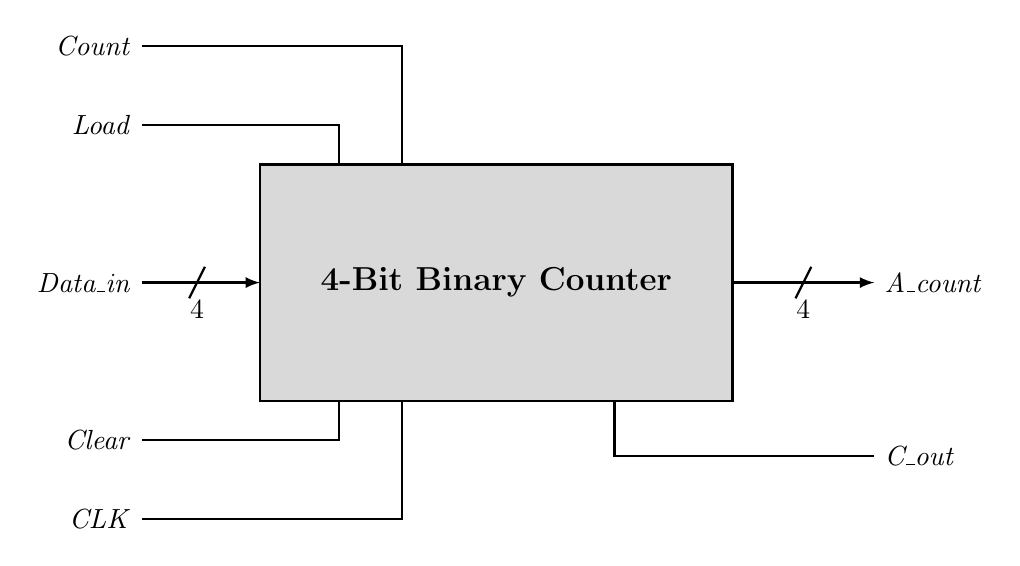
\begin{tikzpicture}[>=latex, thick]

    % ================= মূল ব্লক (Main Block) =================
    % ছবিটিতে ব্লকের ভেতরে একটি টেক্সচার/প্যাটার্ন দেখা যাচ্ছে, এখানে পরিষ্কার ও প্রফেশনাল লুকের জন্য হালকা ছাই রঙ (black!15) দেওয়া হয়েছে।
    \node[draw, rectangle, minimum width=6cm, minimum height=3cm, fill=black!15, font=\large\bfseries] (counter) at (0,0) {4-Bit Binary Counter};

    % ================= উপরের ইনপুটসমূহ (Top Inputs) =================
    % Count
    \draw (-4.5, 3.0) node[left] {\textit{Count}} -- (-1.2, 3.0) -- (-1.2, 1.5);
    % Load
    \draw (-4.5, 2) node[left] {\textit{Load}} -- (-2.0, 2) -- (-2.0, 1.5);

    % ================= বাম পাশের ইনপুট (Left Input) =================
    % Data_in (অ্যারো সহ)
    \draw[->] (-4.5, 0) node[left] {\textit{Data\_in}} -- (-3.0, 0);
    % Data_in এর বাস স্ল্যাশ (Bus Slash)
    \draw (-3.9, -0.2) -- (-3.7, 0.2);
    \node[below] at (-3.8, -0.1) {4};

    % ================= নিচের ইনপুটসমূহ (Bottom Inputs) =================
    % Clear
    \draw (-4.5, -2) node[left] {\textit{Clear}} -- (-2.0, -2) -- (-2.0, -1.5);
    % CLK
    \draw (-4.5, -3.0) node[left] {\textit{CLK}} -- (-1.2, -3.0) -- (-1.2, -1.5);

    % ================= ডান পাশের আউটপুট (Right Output) =================
    % A_count (অ্যারো সহ)
    \draw[->] (3.0, 0) -- (4.8, 0) node[right] {\textit{A\_count}};
    % A_count এর বাস স্ল্যাশ (Bus Slash)
    \draw (3.8, -0.2) -- (4.0, 0.2);
    \node[below] at (3.9, -0.1) {4};

    % ================= নিচের ডান পাশের আউটপুট (Bottom Right Output) =================
    % C_out
    \draw (1.5, -1.5) -- (1.5, -2.2) -- (4.8, -2.2) node[right] {\textit{C\_out}};

\end{tikzpicture}
\end{center}

\mk{12} \yr{CSE 205 | L-2/T-1 | 2015--16}


%% -- Q5: Sync counter 1→4→5→7→2→1 (uncertain year) --
\item Design a synchronous counter with the sequence: $1 \to 4 \to 5 \to 7 \to 2 \to 1$. You need not take any measure for the unused states.
\mk{10} \yr{CSE 205 | L-2/T-1 | 2016--17}

%% -- Q6: Sync counter 0→1→2→5→4→6→0 using SR FF (2017-18) --
\item Design a synchronous counter that counts in the following sequence: $0 \to 1 \to 2 \to 5 \to 4 \to 6 \to 0 \to 1 \to 2 \to \cdots$ Design the counter using SR Flip-Flops and draw the circuit diagram.
\mk{20} \yr{CSE 205 | L-2/T-1 | 2017--18}

%% -- Q7: Sync counter 0→2→4→7→5→3→0 using SR FF (2020-21) --
\item Design a synchronous counter that counts in the sequence $0 \to 2 \to 4 \to 7 \to 5 \to 3 \to 0 \to 2 \to 4 \to \cdots$ Design the counter using SR Flip-Flops and draw the circuit diagram.
\mk{20} \yr{CSE 205 | L-2/T-1 | 2020--21}

%% -- Q7: Synchronous counter 0->2->4->7->5->3->0 with JK, T, D FF (2021-22) --
\item Design a synchronous counter that counts in the following sequence: $0 \to 2 \to 4 \to 7 \to 5 \to 3 \to 0 \to 2 \to 4 \to \ldots$ Design the counter using one JK flip-flop, one T flip-flop and one D flip-flop. Draw the circuit diagram.
\mk{20} \yr{CSE 205 | L-2/T-1 | 2021--22}

%% -- Q8: Synchronous counter 1->2->5->7 with JK FF; analyze unused states (2022-23) --
\item Using JK flip-flops, design a synchronous counter that counts in the following sequence: $1, 2, 5, 7, 1, 2, \ldots$ Analyze the final circuit to ensure that if the circuit enters any of the unused states, after a finite number of clock cycles it comes to a used state.
\mk{13} \yr{CSE 205 | L-2/T-1 | 2022--23}

%% -- Q9: Ring counter initialized incorrectly; analyze and propose correction (2024-25) --
\item A ring counter is initialized incorrectly.
\begin{enumerate}
  \item Analyze the resulting sequence of states.
  \item Propose a circuit modification to ensure automatic correction.
\end{enumerate}
\mk{12} \yr{CSE 205 | L-2/T-1 | 2024--25}


\end{enumerate}

%%──────────────────────────────────────────────────────────────────────
\subtopic{cG}{Synchronous Gray Code Counter}
\label{sub:s7-gray}

\begin{enumerate}

%% -- Q1: 3-bit Gray code counter using JK flip-flops --
\item Develop a synchronous 3-bit counter with a Gray code sequence using JK flip-flops.\\
\textit{(Hint: Gray code count sequence for a 2-bit counter is: $00, 01, 11, 10, 00, 01, \ldots$)}
\mk{18} \yr{CSE 205 | L-2/T-1 | 2011--12}


%% -- Q2: 3-bit synchronous gray code counter (JK FF) --
\item Design a 3-bit synchronous Gray Code Counter using JK Flip-Flops. Show the state diagram, state table, function equations and the circuit diagram.
\mk{15} \yr{CSE 205 | L-2/T-1 | 2014--15}

\end{enumerate}

%%──────────────────────────────────────────────────────────────────────
\subtopic{cG}{Switch-Tail Ring Counter}
\label{sub:s7-ring}

\begin{enumerate}

%% -- Q1: Four-stage switch-tail ring counter --
\item Draw the logic diagram of a four-stage switch-tail ring counter.
\mk{5} \yr{CSE 205 | L-2/T-1 | 2011--12}


%% -- Q2: 5-bit ring counter with shift register; timing diagram (2017-18) --
\item Design a 5-bit ring counter using a shift register and illustrate its operation using a timing diagram.
\mk{10} \yr{CSE 205 | L-2/T-1 | 2017--18}

\end{enumerate}

%%──────────────────────────────────────────────────────────────────────
\subtopic{cG}{Johnson Counter vs Ring Counter}
\label{sub:s7-johnson}

\begin{enumerate}

%% -- Q1: 4-bit Johnson counter, disadvantage, difference from ring --
\item Design a 4-bit Johnson Counter. What is the disadvantage of a Johnson Counter? What is the difference between a Johnson Counter and a Ring Counter?
\mk{10} \yr{CSE 205 | L-2/T-1 | 2014--15}


%% -- Q2: 4-bit Johnson counter with shift register; timing diagram (2018-19) --
\item Design a 4-bit Johnson counter using a shift register and illustrate its operation using a timing diagram.
\mk{7} \yr{CSE 205 | L-2/T-1 | 2018--19}


%% -- Q3: Distinguish ring and Johnson counter; 5-bit versions with timing (2020-21) --
\item Distinguish between a ring counter and a Johnson counter. Design a 5-bit ring counter and a 5-bit Johnson counter using shift registers and illustrate their operation using timing diagrams.
\mk{10} \yr{CSE 205 | L-2/T-1 | 2020--21}
\variant{2019--20}

%% -- Q4: Short note about a ring counter (2022-23) --
\item Write a short note about a ring counter.
\mk{5} \yr{CSE 205 | L-2/T-1 | 2022--23}

\end{enumerate}

%%──────────────────────────────────────────────────────────────────────
\subtopic{cG}{Counter Direction Analysis}
\label{sub:s7-direction}

\begin{enumerate}

%% -- Q1: Up/down direction from counter circuit with VDD --
\item A counter circuit has $V_{DD}$ assigned to Logic~1; the current values of LSB $Q_0$ and MSB $Q_1$ are 0 and~1 respectively. Find the direction (up or down) in which the circuit counts when the next clock pulse occurs. What would have to be altered to make the circuit count in the other direction?

\begin{center}
\begin{circuitikz}[scale=1, transform shape, thick]

  % --- First Flip-Flop (FF0) ---
  % Main Box
  \draw (2, 0) rectangle (4, 3);
  % Internal Pin Labels
  \node[right] at (2, 2.5) {J};
  \node[right] at (2, 1.5) {C};
  \node[right] at (2, 0.5) {K};
  \node[left] at (4, 2.5) {Q};
  \node[left] at (4, 0.5) {$\overline{\text{Q}}$};
  % Clock Triangle
  \draw (2, 1.7) -- (2.2, 1.5) -- (2, 1.3); 
  % Inversion Bubble for Q-bar
  \draw (4.1, 0.5) circle (0.1); 

  % --- Second Flip-Flop (FF1) ---
  % Main Box
  \draw (8, 0) rectangle (10, 3);
  % Internal Pin Labels
  \node[right] at (8, 2.5) {J};
  \node[right] at (8, 1.5) {C};
  \node[right] at (8, 0.5) {K};
  \node[left] at (10, 2.5) {Q};
  \node[left] at (10, 0.5) {$\overline{\text{Q}}$};
  % Clock Triangle
  \draw (8, 1.7) -- (8.2, 1.5) -- (8, 1.3); 
  % Inversion Bubble for Q-bar
  \draw (10.1, 0.5) circle (0.1); 

  % --- External Clock Routing ---
  \draw (0, 1.5) node[left]{Clock} -- (2, 1.5);
  \fill (0.5, 1.5) circle (2pt); % Connection dot for clock split
  % Clock line dropping down and routing to FF1
  \draw (0.5, 1.5) -- (0.5, -1) -- (6.5, -1) -- (6.5, 1.5) -- (8, 1.5);

  % --- VDD & FF0 Inputs Routing ---
  \draw (1.2, 2.5) -- (2, 2.5); % Wire to J
  \draw (1.2, 0.5) -- (2, 0.5); % Wire to K
  \fill (1.2, 2.5) circle (2pt); % Dot at J intersection
  
  % VDD Terminal Rail
  \draw (1.2, 2.5) -- (1.2, 3.5);
  \draw (0.9, 3.5) -- (1.5, 3.5) node[above, midway]{$\text{V}_{\text{DD}}$};
  
  % Vertical wire connecting J & K (with a jump over the clock line)
  \draw (1.2, 2.5) -- (1.2, 1.6);
  \draw (1.2, 1.6) arc (90:270:0.1); % Left-facing jump arc
  \draw (1.2, 1.4) -- (1.2, 0.5);

  % --- FF0 Outputs & FF1 Inputs Routing ---
  % FF0 Q0 Output
  \draw (4, 2.5) -- (5, 2.5) -- (5, 4.5) node[above]{$Q_0$};
  
  % FF0 Q-bar line routed to FF1 (with a jump over the vertical clock wire)
  \draw (4.2, 0.5) -- (6.4, 0.5);
  \draw (6.4, 0.5) arc (180:0:0.1); % Up-facing jump arc
  \draw (6.6, 0.5) -- (7.2, 0.5);
  
  % FF1 J-K input tie connections
  \fill (7.2, 0.5) circle (2pt); % Dot at K intersection
  \draw (7.2, 0.5) -- (8, 0.5);
  \draw (7.2, 2.5) -- (8, 2.5);
  
  % Vertical wire connecting J & K for FF1 (with jump over clock line)
  \draw (7.2, 0.5) -- (7.2, 1.4);
  \draw (7.2, 1.4) arc (-90:-270:0.1); % Left-facing jump arc
  \draw (7.2, 1.6) -- (7.2, 2.5);

  % --- FF1 Outputs Routing ---
  % FF1 Q1 Output
  \draw (10, 2.5) -- (11, 2.5) -- (11, 4.5) node[above]{$Q_1$};
  % FF1 Q-bar open stub
  \draw (10.2, 0.5) -- (11.5, 0.5);

\end{circuitikz}
\end{center}

\mk{7} \yr{CSE 205 | L-2/T-1 | 2015--16}

\end{enumerate}

%%──────────────────────────────────────────────────────────────────────
\subtopic{cG}{Clock Generator / Divider}
\label{sub:s7-clock}

\begin{enumerate}

%% -- Q1: 100 MHz -> 50 MHz and 25 MHz using D FF; timing diagram (2017-18) --
\item Given a 100\,MHz clock signal, derive a circuit using D flip-flops to generate 50\,MHz and 25\,MHz clock signals. Draw a timing diagram for all three clock signals.
\mk{10} \yr{CSE 205 | L-2/T-1 | 2017--18}

\end{enumerate}

%%──────────────────────────────────────────────────────────────────────
\subtopic{cG}{Universal Shift Register}
\label{sub:s7-universal}

\begin{enumerate}

%% -- Q1: 4-bit universal shift register using JK FF --
\item Draw the circuit diagram of a 4-bit universal shift register using JK flip-flops.
\mk{12} \yr{CSE 205 | L-2/T-1 | 2012--13}


%% -- Q2: 2-bit register with D FF + 4x1 MUX, mode control s1,s0 --
\item Draw the logic diagram of a two-bit register with two D flip-flops and two $4\times1$ multiplexers with mode selection inputs $s_1$ and $s_0$. The register operates with four modes: (00) No change, (01) Complement the two outputs, (10) Clear register to 0 (synchronous), (11) Load parallel data.
\mk{12} \yr{CSE 205 | L-2/T-1 | 2015--16}


%% -- Q3: 3-bit universal shift register with 8 modes (s2,s1,s0) (2016-17) --
\item Draw the logic diagram of a 3-bit universal shift register with mode selection inputs $s_2$, $s_1$, $s_0$. The register operates with eight modes: (000) No change, (001) Invert all bits, (010) Set all bits to 0, (011) Set all bits to 1, (100) Parallel load, (101) Shift left, (110) Shift right, (111) No change.
\mk{15} \yr{CSE 205 | L-2/T-1 | 2016--17}

%% -- Q4: 4-bit shift register module with decoder and D FF; 4 modes (2021-22) --
\item Use a 2-to-4 decoder, NAND gates and edge triggered D flip-flops to design a 4-bit shift register module that has the following functions:
\begin{center}
\begin{tabular}{|c|c|l|}
\hline
$S_1$ & $S_0$ & Mode \\
\hline
0 & 0 & Shift right (all 4 bits)\\
0 & 1 & Shift left (all 4 bits)\\
1 & 0 & Synchronous common clear \\
1 & 1 & Synchronous parallel load \\
\hline
\end{tabular}
\end{center}
\mk{10} \yr{CSE 205 | L-2/T-1 | 2021--22}

%% -- Q5: 4-bit universal shift register using MUX and D FF (2024-25) --
\item Design a 4-bit universal shift register using multiplexers and D flip-flops.
\mk{13} \yr{CSE 205 | L-2/T-1 | 2024--25}

%% -- Q6: Compare hardware efficiency of universal vs dedicated shift registers (2024-25) --
\item Compare the hardware efficiency and flexibility of universal shift registers with dedicated shift registers in complex digital systems.
\mk{7} \yr{CSE 205 | L-2/T-1 | 2024--25}

\end{enumerate}

%%──────────────────────────────────────────────────────────────────────
\subtopic{cG}{Serial Adder \& Serial Subtractor}
\label{sub:s7-serial}

\begin{enumerate}

%% -- Q1: Serial adder with clock-by-clock trace (0101 + 0011) --
\item Draw the logic diagram of a serial adder. Show the values of inputs and outputs of all components (e.g., flip-flop, register) used in the design after every clock pulse while adding the following two numbers: $0101$ and $0011$.
\mk{6+6} \yr{CSE 205 | L-2/T-1 | 2011--12, 2012--13}

%% -- Q2: Serial subtractor (B from A in shift registers) --
\item Design a serial subtractor that subtracts the content of register $B$ from the content of register $A$, where the contents of $A$ and $B$ are stored in individual shift registers. The result of the subtraction is stored in the shift register representing $A$. (Both $A$ and $B$ are 4-bit binary numbers.)
\mk{10} \yr{CSE 205 | L-2/T-1 | 2013--14}


%% -- Q3: Serial adder for two 4-bit numbers (2016-17) --
\item Design a serial adder that computes the sum of two 4-bit binary numbers $A$ and $B$ stored in individual shift registers. The result of the addition is stored in the shift register representing $A$. Use the sequential logic design procedure.
\mk{10} \yr{CSE 205 | L-2/T-1 | 2016--17}

%% -- Q4: Serial adder (repeat 2017-18) --
\item Design a serial adder that computes the sum of two 4-bit binary numbers $A$ and $B$ stored in individual shift registers. The result of the addition is stored in the shift register representing $A$.
\mk{10} \yr{CSE 205 | L-2/T-1 | 2017--18}

%% -- Q5: Serial subtractor A-B with JK FF (2021-22) --
\item Design a serial subtractor that will perform the operation $A - B$, where $A = a_{n-1}\ldots a_1 a_0$ and $B = b_{n-1}\ldots b_1 b_0$. The operands are applied to the serial subtractor sequentially, beginning with bits $a_0$ and $b_0$. Use JK flip-flops in your design.
\mk{10} \yr{CSE 205 | L-2/T-1 | 2021--22}

%% -- Q6: Sequential circuit to copy shift register A to B (2022-23) --
\item Design a sequential circuit to copy the content of shift register $A$ to shift register $B$. Use a block diagram to represent the shift register in the diagram.
\mk{12} \yr{CSE 205 | L-2/T-1 | 2022--23}

%% -- Q7: 4-bit shift register for serial data transmission; timing and error propagation (2024-25) --
\item A 4-bit shift register is used for serial data transmission.
\begin{enumerate}
  \item Analyze the timing relationship between input data, clock and output.
  \item Explain how errors may propagate in serial communication using shift registers.
\end{enumerate}
\mk{16} \yr{CSE 205 | L-2/T-1 | 2024--25}

\end{enumerate}


%% ══════════════════════════════════════════════════════════════════════
%%  SECTION 8: MEMORY & PROGRAMMABLE LOGIC
%% ══════════════════════════════════════════════════════════════════════
\secdivider{Memory \& Programmable Logic}{RAM, ROM, Address Multiplexing, PLA Design}{cH}{cyan!30!black}

\markboth{S8: Memory \& Programmable Logic}{S8: Memory \& Programmable Logic}
\label{sec:S8}
\titleformat{\section}{\large\bfseries\color{cH}}{}{0em}{}[\titlerule]
\section*{S8 \quad Memory \& Programmable Logic}
\addcontentsline{toc}{section}{S8: Memory \& Programmable Logic}

%%──────────────────────────────────────────────────────────────────────
\subtopic{cH}{ROM Design \& Expansion}
\label{sub:s8-rom}

\begin{enumerate}

%% -- Q1: 128x4 ROM using 32x4 ROMs --
\item You have several $32 \times 4$ ROMs in the laboratory. Each ROM can be enabled/disabled using a 1/0 signal respectively. How would you implement a $128 \times 4$ ROM using the available ROMs? You may use any additional circuitry if needed.
\mk{10} \yr{CSE 205 | L-2/T-1 | 2013--14}

\end{enumerate}

%%──────────────────────────────────────────────────────────────────────
\subtopic{cH}{PLA Design}
\label{sub:s8-pla}

\begin{enumerate}

%% -- Q1: PLA for three Boolean functions --
\item Implement the following three Boolean functions with a PLA:
\begin{align*}
  F_1 &= \Sigma\,(0,1,2,4) \\
  F_2 &= \Sigma\,(0,5,6,7) \\
  F_3 &= \Sigma\,(0,3,5,7)
\end{align*}
\mk{15} \yr{CSE 205 | L-2/T-1 | 2011--12}

%% -- Q2: PLA program table for 3-bit squarer --
\item Derive the PLA program table for a combinational circuit that squares a 3-bit binary number. Minimize the number of product terms.
\mk{25} \yr{CSE 205 | L-2/T-1 | 2013--14}


%% -- Q3: ROM vs PLA; PLA for F1,F2 --
\item Write the difference between ROM and PLA. A combinational circuit is defined by the following functions:
\begin{align*}
  F_1(A,B,C) &= \Sigma\,(0,1,2,4) \\
  F_2(A,B,C) &= \Sigma\,(0,5,6,7)
\end{align*}
Implement the circuit with a PLA having three inputs, four product terms and two outputs.
\mk{5+10} \yr{CSE 205 | L-2/T-1 | 2014--15}


%% -- Q4: PLA analysis -- find F1, F2, programming table --
\item For a given Programmable Logic Array (PLA), find the function expressions for $F_1$ and $F_2$ and show the PLA programming table.

\begin{center}
  \begin{circuitikz}[scale=0.9, transform shape]
  
  % Vertical lines for inputs (C, C', B, B', A, A' from left to right based on the diagram)
  \foreach \x/\label in {2/C, 2.5/C', 3/B, 3.5/B', 4/A, 4.5/A'} {
      \draw (\x, 0.5) -- (\x, 9);
      \node[below] at (\x, 0.5) {$\label$};
  }

  % Define a custom macro to draw the input buffer/splitter
  % \plasplitter{y_position}{Name}{x_normal}{x_inverted}
  \newcommand{\plasplitter}[4]{
    \draw (0.2, #1) node[left]{#2} -- (0.8, #1);
    \draw (0.8, #1+0.3) -- (0.8, #1-0.3) -- (1.6, #1) -- cycle; % Triangle
    \draw (1.6, #1+0.15) circle (0.08); % Bubble for inverted output
    \draw (1.6+0.08, #1+0.15) -- (#4, #1+0.15); % Line to inverted vertical
    \fill (#4, #1+0.15) circle (2pt); % Connection dot
    \draw (1.6, #1-0.15) -- (#3, #1-0.15); % Line to normal vertical
    \fill (#3, #1-0.15) circle (2pt); % Connection dot
  }
  
  % Draw the 3 input splitters at the top left
  \plasplitter{8.5}{A}{4}{4.5}
  \plasplitter{7.5}{B}{3}{3.5}
  \plasplitter{6.5}{C}{2}{2.5}

  % AND plane (4 AND gates)
  \foreach \y/\id in {5.5/1, 4/2, 2.5/3, 1/4} {
      \node[and port, no input leads] (AND\id) at (6, \y) {};
      \node at (AND\id.center) {\id};
      \draw (1.8, \y) -- (4.9,\y); % Input line to AND gate
      \draw (AND\id.out) -- (10, \y);  % Output line extending right
  }
  
  % Programmable connection dots in the AND plane
  % AND1: C, B, A
 
  \node[or port, rotate=-90, no input leads] (OR1) at (7.5, -1) {};
  \node[or port, rotate=-90, no input leads] (OR2) at (9, -1) {};
  % OR plane (2 OR gates facing downwards)
  % Vertical lines for OR inputs
  \draw (7.5,-.1) -- ++(0,6);
  \draw (9,-.1) -- ++(0,6);


  
  

  % XOR plane (2 XOR gates)
  \node[xor port] (XOR1) at (13, -2) {}; % Top XOR (F1)
  \node[xor port] (XOR2) at (13, -3.5) {}; % Bottom XOR (F2)
  
  % Connect OR outputs to the top inputs of XOR gates
  % Right OR gate connects to F1 (top XOR)
  \draw (OR2.out) |- (XOR1.in 1);
  % Left OR gate connects to F2 (bottom XOR)
  \draw (OR1.out) |- (XOR2.in 1);

  % Programmable polarity lines (0 and 1)
  \draw (10, -0.5) -- (13, -0.5) node[right]{0};
  \draw (10, -1.0) -- (13, -1.0) node[right]{1};
  
  % Connect bottom inputs of XOR gates to polarity lines
  % XOR1 (F1) connects to '1'
  \draw (XOR1.in 2) -- (11, -2.5) -- (11, -0.3);
  
  % XOR2 (F2) connects to '0'
  \draw (XOR2.in 2) -- (10.5, -3.78) -- (10.5, -0.3);

  % Final Outputs
  \node[right] at (XOR1.out) {$F_1$};
  \node[right] at (XOR2.out) {$F_2$};

\end{circuitikz}
\end{center}

\mk{13} \yr{CSE 205 | L-2/T-1 | 2015--16}


%% -- Q5: Security lock using PLA (2018-19) --
\item Design a security lock using PLA which will be opened using the following combinations:
\begin{align*}
  A(x,y,z) &= \Sigma\,(1,3,5,6),\quad B(x,y,z) = \Sigma\,(0,1,6,7) \\
  C(x,y,z) &= \Sigma\,(3,5),\quad D(x,y,z) = \Sigma\,(1,3,4,5,7)
\end{align*}
\mk{12} \yr{CSE 205 | L-2/T-1 | 2018--19}

%% -- Q6: Digital security lock using PLA with BCD-to-Excess-3 conversion (2020-21) --
\item Design a digital security lock using PLA which takes BCD as input and opens after converting the input to Excess-3 code. Use the minimum number of product terms. (Show the fuse map.)
\mk{15} \yr{CSE 205 | L-2/T-1 | 2020--21}


%% -- Q7: PLA design for two 3-variable functions (2019-20) --
\item Design a circuit for the following functions using a Programmable Logic Array (PLA):
\begin{align*}
  A(x,y,z) &= \Sigma\,(0,1,2,5,7) \\
  B(x,y,z) &= \Sigma\,(0,1,3,6,7)
\end{align*}
\mk{10} \yr{CSE 205 | L-2/T-1 | 2019--20}

%% -- Q8: PLA for two functions F1 and F2; 3 inputs, 4 product terms, 2 outputs (2021-22) --
\item A combinational circuit is defined by the following two functions:
\begin{align*}
  F_1(A, B, C) &= \Sigma\,(3, 5, 6, 7) \\
  F_2(A, B, C) &= \Sigma\,(0, 2, 4, 7)
\end{align*}
The circuit needs to be implemented with a PLA having three inputs, four product terms, and two outputs. Show the PLA programming table.
\mk{15} \yr{CSE 205 | L-2/T-1 | 2021--22}

%% -- Q9: PLA programming table for two functions; minimize product terms (2022-23) --
\item Tabulate the PLA programming table for the two Boolean functions listed below. Minimize the numbers of product terms:
\begin{align*}
  F_1(A, B, C) &= \Sigma\,(0, 1, 2, 4) \\
  F_2(A, B, C) &= \Sigma\,(0, 5, 6, 7)
\end{align*}
\mk{15} \yr{CSE 205 | L-2/T-1 | 2022--23}

%% -- Q10: PLA for four functions F1-F4; minimize product terms (2024-25) --
\item Design a PLA to implement the following functions with the minimization of the number of product terms:
\begin{align*}
  F_1(x, y, z) &= \Sigma\,(1,3,5,6),\quad & F_2(x, y, z) &= \Sigma\,(0,1,6,7) \\
  F_3(x, y, z) &= \Sigma\,(3,5),\quad & F_4(x, y, z) &= \Sigma\,(1,2,4,5,7)
\end{align*}
\mk{15} \yr{CSE 205 | L-2/T-1 | 2024--25}

\end{enumerate}

%%──────────────────────────────────────────────────────────────────────
\subtopic{cH}{RAM Design}
\label{sub:s8-ram}

\begin{enumerate}

%% -- Q1: Two-dimensional decoding for 1K word memory; cost optimization (2024-25) --
\item If you use two dimensional decoding for addressing a 1K word memory, can you optimize the cost? Justify your answer.
\mk{8} \yr{CSE 205 | L-2/T-1 | 2024--25}

\end{enumerate}

%% -- S6: Synchronous sequential traffic light and divide-by-three (2023-24) --

%%──────────────────────────────────────────────────────────────────────
\subtopic{cF}{Synchronous Sequential Circuit Design}
\label{sub:s6-sync-design}

\begin{enumerate}

%% -- Q1: Traffic light controller NS-EW; WALK button; D flip-flops (2023-24) --
\item Design a simplified traffic-light controller that switches traffic lights on a crossing where a north-south (NS) street intersects an east-west (EW) street. The input to the controller is the WALK button pushed by pedestrians who want to cross the street. The outputs are two signals NS and EW that control the traffic lights in NS and EW directions. When NS or EW are 0, the red light is on and when they are 1, the green light is on. When there are no pedestrians, $\text{NS}=0$ and $\text{EW}=1$ for 1 minute, followed by $\text{NS}=1$ and $\text{EW}=0$ for 1 minute and so on. When a WALK button is pushed, NS and EW both come 1 for a minute when the present minute expires. After that the NS and EW signals continue alternating. For the traffic-light controller:
	(i) Develop a state diagram and state/output table.
	(ii) Find the transition and excitation tables using S-R flipflops.
	(iii) Draw a circuit diagram.
  \mk{23} \yr{CSE 205 | L-2/T-1 | 2023--24}

%% -- Q2: Divide-by-three counter; counts 1s from input stream; D FF (2023-24) --
\item Design a divide-by-three counter which counts the number of `1's from an input sequence of binary stream. This counter outputs one 1 for every three 1's seen as input (not necessarily in succession). After outputting a 1, it starts counting all over again. Design the counter using D flip-flops.
\mk{12} \yr{CSE 205 | L-2/T-1 | 2023--24}

%% -- Q3: Vending machine synchronous 3Tk; level output; SR FF (2024-25) --
\item Design an automatic vending machine, when the candy bars inside the machine cost 3\,Tk and the machine accepts 1\,Tk and 2\,Tk only. The system accepts the bills sequentially. The circuit produces a level output that delivers the candy whenever the amount received by the machine is 3\,Tk or more. The excess amount is kept deposited for the next candy. Design a synchronous sequential circuit for the vending machine using S-R flip-flops. Provide the circuit diagram as well.
\mk{25} \yr{CSE 205 | L-2/T-1 | 2024--25}

\end{enumerate}


\end{document}